\documentclass[twoside]{book}

% Packages required by doxygen
\usepackage{calc}
\usepackage{doxygen}
\usepackage{graphicx}
\usepackage[utf8]{inputenc}
\usepackage{makeidx}
\usepackage{multicol}
\usepackage{multirow}
\usepackage{textcomp}
\usepackage[table]{xcolor}

% Font selection
\usepackage[T1]{fontenc}
\usepackage{mathptmx}
\usepackage[scaled=.90]{helvet}
\usepackage{courier}
\usepackage{amssymb}
\usepackage{sectsty}
\renewcommand{\familydefault}{\sfdefault}
\allsectionsfont{%
  \fontseries{bc}\selectfont%
  \color{darkgray}%
}
\renewcommand{\DoxyLabelFont}{%
  \fontseries{bc}\selectfont%
  \color{darkgray}%
}

% Page & text layout
\usepackage{geometry}
\geometry{%
  a4paper,%
  top=2.5cm,%
  bottom=2.5cm,%
  left=2.5cm,%
  right=2.5cm%
}
\tolerance=750
\hfuzz=15pt
\hbadness=750
\setlength{\emergencystretch}{15pt}
\setlength{\parindent}{0cm}
\setlength{\parskip}{0.2cm}
\makeatletter
\renewcommand{\paragraph}{%
  \@startsection{paragraph}{4}{0ex}{-1.0ex}{1.0ex}{%
    \normalfont\normalsize\bfseries\SS@parafont%
  }%
}
\renewcommand{\subparagraph}{%
  \@startsection{subparagraph}{5}{0ex}{-1.0ex}{1.0ex}{%
    \normalfont\normalsize\bfseries\SS@subparafont%
  }%
}
\makeatother

% Headers & footers
\usepackage{fancyhdr}
\pagestyle{fancyplain}
\fancyhead[LE]{\fancyplain{}{\bfseries\thepage}}
\fancyhead[CE]{\fancyplain{}{}}
\fancyhead[RE]{\fancyplain{}{\bfseries\leftmark}}
\fancyhead[LO]{\fancyplain{}{\bfseries\rightmark}}
\fancyhead[CO]{\fancyplain{}{}}
\fancyhead[RO]{\fancyplain{}{\bfseries\thepage}}
\fancyfoot[LE]{\fancyplain{}{}}
\fancyfoot[CE]{\fancyplain{}{}}
\fancyfoot[RE]{\fancyplain{}{\bfseries\scriptsize Generated on Mon Mar 2 2015 19\-:43\-:35 for My Project by Doxygen }}
\fancyfoot[LO]{\fancyplain{}{\bfseries\scriptsize Generated on Mon Mar 2 2015 19\-:43\-:35 for My Project by Doxygen }}
\fancyfoot[CO]{\fancyplain{}{}}
\fancyfoot[RO]{\fancyplain{}{}}
\renewcommand{\footrulewidth}{0.4pt}
\renewcommand{\chaptermark}[1]{%
  \markboth{#1}{}%
}
\renewcommand{\sectionmark}[1]{%
  \markright{\thesection\ #1}%
}

% Indices & bibliography
\usepackage{natbib}
\usepackage[titles]{tocloft}
\setcounter{tocdepth}{3}
\setcounter{secnumdepth}{5}
\makeindex

% Hyperlinks (required, but should be loaded last)
\usepackage{ifpdf}
\ifpdf
  \usepackage[pdftex,pagebackref=true]{hyperref}
\else
  \usepackage[ps2pdf,pagebackref=true]{hyperref}
\fi
\hypersetup{%
  colorlinks=true,%
  linkcolor=blue,%
  citecolor=blue,%
  unicode%
}

% Custom commands
\newcommand{\clearemptydoublepage}{%
  \newpage{\pagestyle{empty}\cleardoublepage}%
}


%===== C O N T E N T S =====

\begin{document}

% Titlepage & ToC
\hypersetup{pageanchor=false}
\pagenumbering{roman}
\begin{titlepage}
\vspace*{7cm}
\begin{center}%
{\Large My Project }\\
\vspace*{1cm}
{\large Generated by Doxygen 1.8.6}\\
\vspace*{0.5cm}
{\small Mon Mar 2 2015 19:43:35}\\
\end{center}
\end{titlepage}
\clearemptydoublepage
\tableofcontents
\clearemptydoublepage
\pagenumbering{arabic}
\hypersetup{pageanchor=true}

%--- Begin generated contents ---
\chapter{Namespace Index}
\input{namespaces}
\chapter{Hierarchical Index}
\section{Class Hierarchy}
This inheritance list is sorted roughly, but not completely, alphabetically\-:\begin{DoxyCompactList}
\item \contentsline{section}{Client}{\pageref{structClient}}{}
\item \contentsline{section}{Data}{\pageref{classData}}{}
\item \contentsline{section}{File\-Changes}{\pageref{classFileChanges}}{}
\item \contentsline{section}{File\-History}{\pageref{classFileHistory}}{}
\item \contentsline{section}{File\-Receiving}{\pageref{classFileReceiving}}{}
\item \contentsline{section}{File\-Sharing}{\pageref{classFileSharing}}{}
\item \contentsline{section}{graph}{\pageref{structgraph}}{}
\item \contentsline{section}{Instruction}{\pageref{structInstruction}}{}
\item Q\-Dialog\begin{DoxyCompactList}
\item \contentsline{section}{connecting}{\pageref{classconnecting}}{}
\item \contentsline{section}{file}{\pageref{classfile}}{}
\item \contentsline{section}{fileaccess}{\pageref{classfileaccess}}{}
\item \contentsline{section}{New\-User\-Signup}{\pageref{classNewUserSignup}}{}
\item \contentsline{section}{share}{\pageref{classshare}}{}
\item \contentsline{section}{sharedwithothers}{\pageref{classsharedwithothers}}{}
\end{DoxyCompactList}
\item Q\-Main\-Window\begin{DoxyCompactList}
\item \contentsline{section}{login}{\pageref{classlogin}}{}
\end{DoxyCompactList}
\item \contentsline{section}{qt\-\_\-meta\-\_\-stringdata\-\_\-connecting\-\_\-t}{\pageref{structqt__meta__stringdata__connecting__t}}{}
\item \contentsline{section}{qt\-\_\-meta\-\_\-stringdata\-\_\-file\-\_\-t}{\pageref{structqt__meta__stringdata__file__t}}{}
\item \contentsline{section}{qt\-\_\-meta\-\_\-stringdata\-\_\-fileaccess\-\_\-t}{\pageref{structqt__meta__stringdata__fileaccess__t}}{}
\item \contentsline{section}{qt\-\_\-meta\-\_\-stringdata\-\_\-login\-\_\-t}{\pageref{structqt__meta__stringdata__login__t}}{}
\item \contentsline{section}{qt\-\_\-meta\-\_\-stringdata\-\_\-\-New\-User\-Signup\-\_\-t}{\pageref{structqt__meta__stringdata__NewUserSignup__t}}{}
\item \contentsline{section}{qt\-\_\-meta\-\_\-stringdata\-\_\-share\-\_\-t}{\pageref{structqt__meta__stringdata__share__t}}{}
\item \contentsline{section}{qt\-\_\-meta\-\_\-stringdata\-\_\-sharedwithothers\-\_\-t}{\pageref{structqt__meta__stringdata__sharedwithothers__t}}{}
\item \contentsline{section}{Sharing}{\pageref{structSharing}}{}
\item \contentsline{section}{Sharing\-Giver}{\pageref{structSharingGiver}}{}
\item \contentsline{section}{Sync\-List}{\pageref{structSyncList}}{}
\item \contentsline{section}{Sync\-Manager}{\pageref{classSyncManager}}{}
\item \contentsline{section}{Ui\-\_\-connecting}{\pageref{classUi__connecting}}{}
\begin{DoxyCompactList}
\item \contentsline{section}{Ui\-:\-:connecting}{\pageref{classUi_1_1connecting}}{}
\end{DoxyCompactList}
\item \contentsline{section}{Ui\-\_\-file}{\pageref{classUi__file}}{}
\begin{DoxyCompactList}
\item \contentsline{section}{Ui\-:\-:file}{\pageref{classUi_1_1file}}{}
\end{DoxyCompactList}
\item \contentsline{section}{Ui\-\_\-fileaccess}{\pageref{classUi__fileaccess}}{}
\begin{DoxyCompactList}
\item \contentsline{section}{Ui\-:\-:fileaccess}{\pageref{classUi_1_1fileaccess}}{}
\end{DoxyCompactList}
\item \contentsline{section}{Ui\-\_\-login}{\pageref{classUi__login}}{}
\begin{DoxyCompactList}
\item \contentsline{section}{Ui\-:\-:login}{\pageref{classUi_1_1login}}{}
\end{DoxyCompactList}
\item \contentsline{section}{Ui\-\_\-\-New\-User\-Signup}{\pageref{classUi__NewUserSignup}}{}
\begin{DoxyCompactList}
\item \contentsline{section}{Ui\-:\-:New\-User\-Signup}{\pageref{classUi_1_1NewUserSignup}}{}
\end{DoxyCompactList}
\item \contentsline{section}{Ui\-\_\-share}{\pageref{classUi__share}}{}
\begin{DoxyCompactList}
\item \contentsline{section}{Ui\-:\-:share}{\pageref{classUi_1_1share}}{}
\end{DoxyCompactList}
\item \contentsline{section}{Ui\-\_\-sharedwithothers}{\pageref{classUi__sharedwithothers}}{}
\begin{DoxyCompactList}
\item \contentsline{section}{Ui\-:\-:sharedwithothers}{\pageref{classUi_1_1sharedwithothers}}{}
\end{DoxyCompactList}
\item \contentsline{section}{User\-Files}{\pageref{classUserFiles}}{}
\end{DoxyCompactList}

\chapter{Class Index}
\section{Class List}
Here are the classes, structs, unions and interfaces with brief descriptions\-:\begin{DoxyCompactList}
\item\contentsline{section}{\hyperlink{structClient}{Client} }{\pageref{structClient}}{}
\item\contentsline{section}{\hyperlink{classconnecting}{connecting} }{\pageref{classconnecting}}{}
\item\contentsline{section}{\hyperlink{classUi_1_1connecting}{Ui\-::connecting} }{\pageref{classUi_1_1connecting}}{}
\item\contentsline{section}{\hyperlink{classData}{Data} }{\pageref{classData}}{}
\item\contentsline{section}{\hyperlink{classfile}{file} }{\pageref{classfile}}{}
\item\contentsline{section}{\hyperlink{classUi_1_1file}{Ui\-::file} }{\pageref{classUi_1_1file}}{}
\item\contentsline{section}{\hyperlink{classUi_1_1fileaccess}{Ui\-::fileaccess} }{\pageref{classUi_1_1fileaccess}}{}
\item\contentsline{section}{\hyperlink{classfileaccess}{fileaccess} }{\pageref{classfileaccess}}{}
\item\contentsline{section}{\hyperlink{classFileChanges}{File\-Changes} }{\pageref{classFileChanges}}{}
\item\contentsline{section}{\hyperlink{classFileHistory}{File\-History} }{\pageref{classFileHistory}}{}
\item\contentsline{section}{\hyperlink{classFileReceiving}{File\-Receiving} }{\pageref{classFileReceiving}}{}
\item\contentsline{section}{\hyperlink{classFileSharing}{File\-Sharing} }{\pageref{classFileSharing}}{}
\item\contentsline{section}{\hyperlink{structgraph}{graph} }{\pageref{structgraph}}{}
\item\contentsline{section}{\hyperlink{structInstruction}{Instruction} }{\pageref{structInstruction}}{}
\item\contentsline{section}{\hyperlink{classUi_1_1login}{Ui\-::login} }{\pageref{classUi_1_1login}}{}
\item\contentsline{section}{\hyperlink{classlogin}{login} }{\pageref{classlogin}}{}
\item\contentsline{section}{\hyperlink{classUi_1_1NewUserSignup}{Ui\-::\-New\-User\-Signup} }{\pageref{classUi_1_1NewUserSignup}}{}
\item\contentsline{section}{\hyperlink{classNewUserSignup}{New\-User\-Signup} }{\pageref{classNewUserSignup}}{}
\item\contentsline{section}{\hyperlink{structqt__meta__stringdata__connecting__t}{qt\-\_\-meta\-\_\-stringdata\-\_\-connecting\-\_\-t} }{\pageref{structqt__meta__stringdata__connecting__t}}{}
\item\contentsline{section}{\hyperlink{structqt__meta__stringdata__file__t}{qt\-\_\-meta\-\_\-stringdata\-\_\-file\-\_\-t} }{\pageref{structqt__meta__stringdata__file__t}}{}
\item\contentsline{section}{\hyperlink{structqt__meta__stringdata__fileaccess__t}{qt\-\_\-meta\-\_\-stringdata\-\_\-fileaccess\-\_\-t} }{\pageref{structqt__meta__stringdata__fileaccess__t}}{}
\item\contentsline{section}{\hyperlink{structqt__meta__stringdata__login__t}{qt\-\_\-meta\-\_\-stringdata\-\_\-login\-\_\-t} }{\pageref{structqt__meta__stringdata__login__t}}{}
\item\contentsline{section}{\hyperlink{structqt__meta__stringdata__NewUserSignup__t}{qt\-\_\-meta\-\_\-stringdata\-\_\-\-New\-User\-Signup\-\_\-t} }{\pageref{structqt__meta__stringdata__NewUserSignup__t}}{}
\item\contentsline{section}{\hyperlink{structqt__meta__stringdata__share__t}{qt\-\_\-meta\-\_\-stringdata\-\_\-share\-\_\-t} }{\pageref{structqt__meta__stringdata__share__t}}{}
\item\contentsline{section}{\hyperlink{structqt__meta__stringdata__sharedwithothers__t}{qt\-\_\-meta\-\_\-stringdata\-\_\-sharedwithothers\-\_\-t} }{\pageref{structqt__meta__stringdata__sharedwithothers__t}}{}
\item\contentsline{section}{\hyperlink{classUi_1_1share}{Ui\-::share} }{\pageref{classUi_1_1share}}{}
\item\contentsline{section}{\hyperlink{classshare}{share} }{\pageref{classshare}}{}
\item\contentsline{section}{\hyperlink{classUi_1_1sharedwithothers}{Ui\-::sharedwithothers} }{\pageref{classUi_1_1sharedwithothers}}{}
\item\contentsline{section}{\hyperlink{classsharedwithothers}{sharedwithothers} }{\pageref{classsharedwithothers}}{}
\item\contentsline{section}{\hyperlink{structSharing}{Sharing} }{\pageref{structSharing}}{}
\item\contentsline{section}{\hyperlink{structSharingGiver}{Sharing\-Giver} }{\pageref{structSharingGiver}}{}
\item\contentsline{section}{\hyperlink{structSyncList}{Sync\-List} }{\pageref{structSyncList}}{}
\item\contentsline{section}{\hyperlink{classSyncManager}{Sync\-Manager} }{\pageref{classSyncManager}}{}
\item\contentsline{section}{\hyperlink{classUi__connecting}{Ui\-\_\-connecting} }{\pageref{classUi__connecting}}{}
\item\contentsline{section}{\hyperlink{classUi__file}{Ui\-\_\-file} }{\pageref{classUi__file}}{}
\item\contentsline{section}{\hyperlink{classUi__fileaccess}{Ui\-\_\-fileaccess} }{\pageref{classUi__fileaccess}}{}
\item\contentsline{section}{\hyperlink{classUi__login}{Ui\-\_\-login} }{\pageref{classUi__login}}{}
\item\contentsline{section}{\hyperlink{classUi__NewUserSignup}{Ui\-\_\-\-New\-User\-Signup} }{\pageref{classUi__NewUserSignup}}{}
\item\contentsline{section}{\hyperlink{classUi__share}{Ui\-\_\-share} }{\pageref{classUi__share}}{}
\item\contentsline{section}{\hyperlink{classUi__sharedwithothers}{Ui\-\_\-sharedwithothers} }{\pageref{classUi__sharedwithothers}}{}
\item\contentsline{section}{\hyperlink{classUserFiles}{User\-Files} }{\pageref{classUserFiles}}{}
\end{DoxyCompactList}

\chapter{File Index}
\section{File List}
Here is a list of all files with brief descriptions\-:\begin{DoxyCompactList}
\item\contentsline{section}{\hyperlink{ClientCombined_8cpp}{Client\-Combined.\-cpp} }{\pageref{ClientCombined_8cpp}}{}
\item\contentsline{section}{\hyperlink{ClientCombined_8h}{Client\-Combined.\-h} }{\pageref{ClientCombined_8h}}{}
\item\contentsline{section}{\hyperlink{connecting_8cpp}{connecting.\-cpp} }{\pageref{connecting_8cpp}}{}
\item\contentsline{section}{\hyperlink{connecting_8h}{connecting.\-h} }{\pageref{connecting_8h}}{}
\item\contentsline{section}{\hyperlink{file_8cpp}{file.\-cpp} }{\pageref{file_8cpp}}{}
\item\contentsline{section}{\hyperlink{file_8h}{file.\-h} }{\pageref{file_8h}}{}
\item\contentsline{section}{\hyperlink{fileaccess_8cpp}{fileaccess.\-cpp} }{\pageref{fileaccess_8cpp}}{}
\item\contentsline{section}{\hyperlink{fileaccess_8h}{fileaccess.\-h} }{\pageref{fileaccess_8h}}{}
\item\contentsline{section}{\hyperlink{FileChanges_8cpp}{File\-Changes.\-cpp} }{\pageref{FileChanges_8cpp}}{}
\item\contentsline{section}{\hyperlink{FileChanges_8h}{File\-Changes.\-h} }{\pageref{FileChanges_8h}}{}
\item\contentsline{section}{\hyperlink{FileHistory_8cpp}{File\-History.\-cpp} }{\pageref{FileHistory_8cpp}}{}
\item\contentsline{section}{\hyperlink{FileHistory_8h}{File\-History.\-h} }{\pageref{FileHistory_8h}}{}
\item\contentsline{section}{\hyperlink{FileReceiving_8cpp}{File\-Receiving.\-cpp} }{\pageref{FileReceiving_8cpp}}{}
\item\contentsline{section}{\hyperlink{FileReceiving_8h}{File\-Receiving.\-h} }{\pageref{FileReceiving_8h}}{}
\item\contentsline{section}{\hyperlink{FileSharing_8cpp}{File\-Sharing.\-cpp} }{\pageref{FileSharing_8cpp}}{}
\item\contentsline{section}{\hyperlink{FileSharing_8h}{File\-Sharing.\-h} }{\pageref{FileSharing_8h}}{}
\item\contentsline{section}{\hyperlink{filesonserver_8cpp}{filesonserver.\-cpp} }{\pageref{filesonserver_8cpp}}{}
\item\contentsline{section}{\hyperlink{filesonserver_8h}{filesonserver.\-h} }{\pageref{filesonserver_8h}}{}
\item\contentsline{section}{\hyperlink{login_8cpp}{login.\-cpp} }{\pageref{login_8cpp}}{}
\item\contentsline{section}{\hyperlink{login_8h}{login.\-h} }{\pageref{login_8h}}{}
\item\contentsline{section}{\hyperlink{main_8cpp}{main.\-cpp} }{\pageref{main_8cpp}}{}
\item\contentsline{section}{\hyperlink{moc__connecting_8cpp}{moc\-\_\-connecting.\-cpp} }{\pageref{moc__connecting_8cpp}}{}
\item\contentsline{section}{\hyperlink{moc__file_8cpp}{moc\-\_\-file.\-cpp} }{\pageref{moc__file_8cpp}}{}
\item\contentsline{section}{\hyperlink{moc__fileaccess_8cpp}{moc\-\_\-fileaccess.\-cpp} }{\pageref{moc__fileaccess_8cpp}}{}
\item\contentsline{section}{\hyperlink{moc__login_8cpp}{moc\-\_\-login.\-cpp} }{\pageref{moc__login_8cpp}}{}
\item\contentsline{section}{\hyperlink{moc__newusersignup_8cpp}{moc\-\_\-newusersignup.\-cpp} }{\pageref{moc__newusersignup_8cpp}}{}
\item\contentsline{section}{\hyperlink{moc__share_8cpp}{moc\-\_\-share.\-cpp} }{\pageref{moc__share_8cpp}}{}
\item\contentsline{section}{\hyperlink{moc__sharedwithothers_8cpp}{moc\-\_\-sharedwithothers.\-cpp} }{\pageref{moc__sharedwithothers_8cpp}}{}
\item\contentsline{section}{\hyperlink{newusersignup_8cpp}{newusersignup.\-cpp} }{\pageref{newusersignup_8cpp}}{}
\item\contentsline{section}{\hyperlink{newusersignup_8h}{newusersignup.\-h} }{\pageref{newusersignup_8h}}{}
\item\contentsline{section}{\hyperlink{share_8cpp}{share.\-cpp} }{\pageref{share_8cpp}}{}
\item\contentsline{section}{\hyperlink{share_8h}{share.\-h} }{\pageref{share_8h}}{}
\item\contentsline{section}{\hyperlink{sharedwithothers_8cpp}{sharedwithothers.\-cpp} }{\pageref{sharedwithothers_8cpp}}{}
\item\contentsline{section}{\hyperlink{sharedwithothers_8h}{sharedwithothers.\-h} }{\pageref{sharedwithothers_8h}}{}
\item\contentsline{section}{\hyperlink{SyncManager_8cpp}{Sync\-Manager.\-cpp} }{\pageref{SyncManager_8cpp}}{}
\item\contentsline{section}{\hyperlink{SyncManager_8h}{Sync\-Manager.\-h} }{\pageref{SyncManager_8h}}{}
\item\contentsline{section}{\hyperlink{ui__connecting_8h}{ui\-\_\-connecting.\-h} }{\pageref{ui__connecting_8h}}{}
\item\contentsline{section}{\hyperlink{ui__file_8h}{ui\-\_\-file.\-h} }{\pageref{ui__file_8h}}{}
\item\contentsline{section}{\hyperlink{ui__fileaccess_8h}{ui\-\_\-fileaccess.\-h} }{\pageref{ui__fileaccess_8h}}{}
\item\contentsline{section}{\hyperlink{ui__login_8h}{ui\-\_\-login.\-h} }{\pageref{ui__login_8h}}{}
\item\contentsline{section}{\hyperlink{ui__newusersignup_8h}{ui\-\_\-newusersignup.\-h} }{\pageref{ui__newusersignup_8h}}{}
\item\contentsline{section}{\hyperlink{ui__share_8h}{ui\-\_\-share.\-h} }{\pageref{ui__share_8h}}{}
\item\contentsline{section}{\hyperlink{ui__sharedwithothers_8h}{ui\-\_\-sharedwithothers.\-h} }{\pageref{ui__sharedwithothers_8h}}{}
\item\contentsline{section}{\hyperlink{UserFiles_8cpp}{User\-Files.\-cpp} }{\pageref{UserFiles_8cpp}}{}
\item\contentsline{section}{\hyperlink{UserFiles_8h}{User\-Files.\-h} }{\pageref{UserFiles_8h}}{}
\end{DoxyCompactList}

\chapter{Namespace Documentation}
\hypertarget{namespaceUi}{\section{Ui Namespace Reference}
\label{namespaceUi}\index{Ui@{Ui}}
}
\subsection*{Classes}
\begin{DoxyCompactItemize}
\item 
class \hyperlink{classUi_1_1allusers}{allusers}
\item 
class \hyperlink{classUi_1_1OnlineUsers}{Online\-Users}
\item 
class \hyperlink{classUi_1_1server}{server}
\item 
class \hyperlink{classUi_1_1serverfilesandfolders}{serverfilesandfolders}
\end{DoxyCompactItemize}

\chapter{Class Documentation}
\hypertarget{classallusers}{\section{allusers Class Reference}
\label{classallusers}\index{allusers@{allusers}}
}


{\ttfamily \#include $<$allusers.\-h$>$}

Inheritance diagram for allusers\-:\begin{figure}[H]
\begin{center}
\leavevmode
\includegraphics[height=2.000000cm]{classallusers}
\end{center}
\end{figure}
\subsection*{Public Member Functions}
\begin{DoxyCompactItemize}
\item 
\hyperlink{classallusers_ac0f3d7bc4255531242d196f2793f6582}{allusers} (Q\-Widget $\ast$parent=0)
\item 
\hyperlink{classallusers_a80c2b459737105578d841f20b29c8ace}{$\sim$allusers} ()
\end{DoxyCompactItemize}
\subsection*{Private Slots}
\begin{DoxyCompactItemize}
\item 
void \hyperlink{classallusers_ae4418ba485da07d651241cbecbd0414a}{on\-\_\-push\-Button\-\_\-2\-\_\-clicked} ()
\end{DoxyCompactItemize}
\subsection*{Private Attributes}
\begin{DoxyCompactItemize}
\item 
\hyperlink{classUi_1_1allusers}{Ui\-::allusers} $\ast$ \hyperlink{classallusers_a3a8127e4f183a49f532a696a341efdbf}{ui}
\end{DoxyCompactItemize}


\subsection{Constructor \& Destructor Documentation}
\hypertarget{classallusers_ac0f3d7bc4255531242d196f2793f6582}{\index{allusers@{allusers}!allusers@{allusers}}
\index{allusers@{allusers}!allusers@{allusers}}
\subsubsection[{allusers}]{\setlength{\rightskip}{0pt plus 5cm}allusers\-::allusers (
\begin{DoxyParamCaption}
\item[{Q\-Widget $\ast$}]{parent = {\ttfamily 0}}
\end{DoxyParamCaption}
)\hspace{0.3cm}{\ttfamily [explicit]}}}\label{classallusers_ac0f3d7bc4255531242d196f2793f6582}
\hypertarget{classallusers_a80c2b459737105578d841f20b29c8ace}{\index{allusers@{allusers}!$\sim$allusers@{$\sim$allusers}}
\index{$\sim$allusers@{$\sim$allusers}!allusers@{allusers}}
\subsubsection[{$\sim$allusers}]{\setlength{\rightskip}{0pt plus 5cm}allusers\-::$\sim$allusers (
\begin{DoxyParamCaption}
{}
\end{DoxyParamCaption}
)}}\label{classallusers_a80c2b459737105578d841f20b29c8ace}


\subsection{Member Function Documentation}
\hypertarget{classallusers_ae4418ba485da07d651241cbecbd0414a}{\index{allusers@{allusers}!on\-\_\-push\-Button\-\_\-2\-\_\-clicked@{on\-\_\-push\-Button\-\_\-2\-\_\-clicked}}
\index{on\-\_\-push\-Button\-\_\-2\-\_\-clicked@{on\-\_\-push\-Button\-\_\-2\-\_\-clicked}!allusers@{allusers}}
\subsubsection[{on\-\_\-push\-Button\-\_\-2\-\_\-clicked}]{\setlength{\rightskip}{0pt plus 5cm}void allusers\-::on\-\_\-push\-Button\-\_\-2\-\_\-clicked (
\begin{DoxyParamCaption}
{}
\end{DoxyParamCaption}
)\hspace{0.3cm}{\ttfamily [private]}, {\ttfamily [slot]}}}\label{classallusers_ae4418ba485da07d651241cbecbd0414a}


\subsection{Member Data Documentation}
\hypertarget{classallusers_a3a8127e4f183a49f532a696a341efdbf}{\index{allusers@{allusers}!ui@{ui}}
\index{ui@{ui}!allusers@{allusers}}
\subsubsection[{ui}]{\setlength{\rightskip}{0pt plus 5cm}{\bf Ui\-::allusers}$\ast$ allusers\-::ui\hspace{0.3cm}{\ttfamily [private]}}}\label{classallusers_a3a8127e4f183a49f532a696a341efdbf}


The documentation for this class was generated from the following files\-:\begin{DoxyCompactItemize}
\item 
\hyperlink{allusers_8h}{allusers.\-h}\item 
\hyperlink{allusers_8cpp}{allusers.\-cpp}\end{DoxyCompactItemize}

\hypertarget{classUi_1_1allusers}{\section{Ui\-:\-:allusers Class Reference}
\label{classUi_1_1allusers}\index{Ui\-::allusers@{Ui\-::allusers}}
}


{\ttfamily \#include $<$ui\-\_\-allusers.\-h$>$}

Inheritance diagram for Ui\-:\-:allusers\-:\begin{figure}[H]
\begin{center}
\leavevmode
\includegraphics[height=2.000000cm]{classUi_1_1allusers}
\end{center}
\end{figure}
\subsection*{Additional Inherited Members}


The documentation for this class was generated from the following file\-:\begin{DoxyCompactItemize}
\item 
\hyperlink{ui__allusers_8h}{ui\-\_\-allusers.\-h}\end{DoxyCompactItemize}

\hypertarget{classFileHistory}{\section{File\-History Class Reference}
\label{classFileHistory}\index{File\-History@{File\-History}}
}


{\ttfamily \#include $<$File\-History.\-h$>$}

\subsection*{Public Member Functions}
\begin{DoxyCompactItemize}
\item 
\hyperlink{classFileHistory_a841820a546629b57a1c779b6d1fd5b01}{File\-History} ()
\item 
\hyperlink{classFileHistory_aa310b68872f8288b9da8a93494d8f525}{File\-History} (std\-::string)
\item 
std\-::string \hyperlink{classFileHistory_abd579dba633254deeec041baca818dd4}{Get\-Folder} ()
\item 
std\-::vector$<$ std\-::pair\\*
$<$ std\-::string, int $>$ $>$ \hyperlink{classFileHistory_a3d1903578989dfc361949bc15a838916}{Get\-File\-Time\-Base} ()
\item 
int \hyperlink{classFileHistory_aef61a14e143844cc16549984ab58a6da}{Get\-Data\-Time} ()
\item 
int \hyperlink{classFileHistory_af21dcb68d35717715e21d9121fda54c3}{Get\-Number\-Of\-Files} ()
\item 
std\-::pair$<$ std\-::string, int $>$ \hyperlink{classFileHistory_a23e62c1567a2a2ede14e028c917a867d}{Get\-Nth\-Info} (int)
\item 
std\-::string \hyperlink{classFileHistory_afeea4550ec1a66b978b69e8baccd3ab5}{Get\-Nth\-Name} (int)
\item 
int \hyperlink{classFileHistory_abc507e5a818fde5c73608d1126eb43bf}{Get\-Nth\-Time} (int)
\item 
void \hyperlink{classFileHistory_a111c5a71865ac87637e1bb22c0fa7a2c}{Set\-Data\-Time} (int)
\item 
void \hyperlink{classFileHistory_a22a0e9aa366f2f8cd0c748cce6d16e19}{Set\-Folder\-Location} (std\-::string)
\item 
void \hyperlink{classFileHistory_af78b8284b8188ff9c29d875e4e630ba1}{Set\-File\-Time\-Base} (std\-::vector$<$ std\-::pair$<$ std\-::string, int $>$ $>$)
\item 
void \hyperlink{classFileHistory_a433153884b5c84c40cf09e9dc0783a7d}{Set\-Nth\-Info} (int, std\-::string, int)
\item 
void \hyperlink{classFileHistory_a231ec4de86666d32c332ccd8b129007d}{Set\-Nth\-File} (int, std\-::string)
\item 
void \hyperlink{classFileHistory_a34e0887629722064f1e077cf7ceff7aa}{Set\-Nth\-Time} (int, int)
\item 
void \hyperlink{classFileHistory_a352c832218a7912402142e80a6563233}{Load\-File\-Time\-Base} ()
\item 
void \hyperlink{classFileHistory_a0e797c6bfddd9a9ac2ef73ca2ccf5ea3}{Load\-From\-File\-Base} (std\-::string)
\item 
void \hyperlink{classFileHistory_aa51ad2b7dfd56927ae83f8abbd2fdbc1}{Store\-To\-File\-Base} (std\-::string)
\end{DoxyCompactItemize}
\subsection*{Private Attributes}
\begin{DoxyCompactItemize}
\item 
std\-::string \hyperlink{classFileHistory_a4ed9b51579a45e657ba6e1dbb4d2e7a7}{Folder\-Location}
\item 
int \hyperlink{classFileHistory_ac054d9b23889c2d64faebfbb67bcf444}{Time\-Of\-Data}
\item 
std\-::vector$<$ std\-::pair\\*
$<$ std\-::string, int $>$ $>$ \hyperlink{classFileHistory_ac4ce01b2c30fedd241d93107f34c3750}{File\-Time\-Base}
\end{DoxyCompactItemize}


\subsection{Constructor \& Destructor Documentation}
\hypertarget{classFileHistory_a841820a546629b57a1c779b6d1fd5b01}{\index{File\-History@{File\-History}!File\-History@{File\-History}}
\index{File\-History@{File\-History}!FileHistory@{File\-History}}
\subsubsection[{File\-History}]{\setlength{\rightskip}{0pt plus 5cm}File\-History\-::\-File\-History (
\begin{DoxyParamCaption}
{}
\end{DoxyParamCaption}
)}}\label{classFileHistory_a841820a546629b57a1c779b6d1fd5b01}
\hypertarget{classFileHistory_aa310b68872f8288b9da8a93494d8f525}{\index{File\-History@{File\-History}!File\-History@{File\-History}}
\index{File\-History@{File\-History}!FileHistory@{File\-History}}
\subsubsection[{File\-History}]{\setlength{\rightskip}{0pt plus 5cm}File\-History\-::\-File\-History (
\begin{DoxyParamCaption}
\item[{std\-::string}]{location}
\end{DoxyParamCaption}
)}}\label{classFileHistory_aa310b68872f8288b9da8a93494d8f525}


\subsection{Member Function Documentation}
\hypertarget{classFileHistory_aef61a14e143844cc16549984ab58a6da}{\index{File\-History@{File\-History}!Get\-Data\-Time@{Get\-Data\-Time}}
\index{Get\-Data\-Time@{Get\-Data\-Time}!FileHistory@{File\-History}}
\subsubsection[{Get\-Data\-Time}]{\setlength{\rightskip}{0pt plus 5cm}int File\-History\-::\-Get\-Data\-Time (
\begin{DoxyParamCaption}
{}
\end{DoxyParamCaption}
)}}\label{classFileHistory_aef61a14e143844cc16549984ab58a6da}
\hypertarget{classFileHistory_a3d1903578989dfc361949bc15a838916}{\index{File\-History@{File\-History}!Get\-File\-Time\-Base@{Get\-File\-Time\-Base}}
\index{Get\-File\-Time\-Base@{Get\-File\-Time\-Base}!FileHistory@{File\-History}}
\subsubsection[{Get\-File\-Time\-Base}]{\setlength{\rightskip}{0pt plus 5cm}std\-::vector$<$ std\-::pair$<$ std\-::string, int $>$ $>$ File\-History\-::\-Get\-File\-Time\-Base (
\begin{DoxyParamCaption}
{}
\end{DoxyParamCaption}
)}}\label{classFileHistory_a3d1903578989dfc361949bc15a838916}
\hypertarget{classFileHistory_abd579dba633254deeec041baca818dd4}{\index{File\-History@{File\-History}!Get\-Folder@{Get\-Folder}}
\index{Get\-Folder@{Get\-Folder}!FileHistory@{File\-History}}
\subsubsection[{Get\-Folder}]{\setlength{\rightskip}{0pt plus 5cm}std\-::string File\-History\-::\-Get\-Folder (
\begin{DoxyParamCaption}
{}
\end{DoxyParamCaption}
)}}\label{classFileHistory_abd579dba633254deeec041baca818dd4}
\hypertarget{classFileHistory_a23e62c1567a2a2ede14e028c917a867d}{\index{File\-History@{File\-History}!Get\-Nth\-Info@{Get\-Nth\-Info}}
\index{Get\-Nth\-Info@{Get\-Nth\-Info}!FileHistory@{File\-History}}
\subsubsection[{Get\-Nth\-Info}]{\setlength{\rightskip}{0pt plus 5cm}std\-::pair$<$ std\-::string, int $>$ File\-History\-::\-Get\-Nth\-Info (
\begin{DoxyParamCaption}
\item[{int}]{n}
\end{DoxyParamCaption}
)}}\label{classFileHistory_a23e62c1567a2a2ede14e028c917a867d}
\hypertarget{classFileHistory_afeea4550ec1a66b978b69e8baccd3ab5}{\index{File\-History@{File\-History}!Get\-Nth\-Name@{Get\-Nth\-Name}}
\index{Get\-Nth\-Name@{Get\-Nth\-Name}!FileHistory@{File\-History}}
\subsubsection[{Get\-Nth\-Name}]{\setlength{\rightskip}{0pt plus 5cm}std\-::string File\-History\-::\-Get\-Nth\-Name (
\begin{DoxyParamCaption}
\item[{int}]{n}
\end{DoxyParamCaption}
)}}\label{classFileHistory_afeea4550ec1a66b978b69e8baccd3ab5}
\hypertarget{classFileHistory_abc507e5a818fde5c73608d1126eb43bf}{\index{File\-History@{File\-History}!Get\-Nth\-Time@{Get\-Nth\-Time}}
\index{Get\-Nth\-Time@{Get\-Nth\-Time}!FileHistory@{File\-History}}
\subsubsection[{Get\-Nth\-Time}]{\setlength{\rightskip}{0pt plus 5cm}int File\-History\-::\-Get\-Nth\-Time (
\begin{DoxyParamCaption}
\item[{int}]{n}
\end{DoxyParamCaption}
)}}\label{classFileHistory_abc507e5a818fde5c73608d1126eb43bf}
\hypertarget{classFileHistory_af21dcb68d35717715e21d9121fda54c3}{\index{File\-History@{File\-History}!Get\-Number\-Of\-Files@{Get\-Number\-Of\-Files}}
\index{Get\-Number\-Of\-Files@{Get\-Number\-Of\-Files}!FileHistory@{File\-History}}
\subsubsection[{Get\-Number\-Of\-Files}]{\setlength{\rightskip}{0pt plus 5cm}int File\-History\-::\-Get\-Number\-Of\-Files (
\begin{DoxyParamCaption}
{}
\end{DoxyParamCaption}
)}}\label{classFileHistory_af21dcb68d35717715e21d9121fda54c3}
\hypertarget{classFileHistory_a352c832218a7912402142e80a6563233}{\index{File\-History@{File\-History}!Load\-File\-Time\-Base@{Load\-File\-Time\-Base}}
\index{Load\-File\-Time\-Base@{Load\-File\-Time\-Base}!FileHistory@{File\-History}}
\subsubsection[{Load\-File\-Time\-Base}]{\setlength{\rightskip}{0pt plus 5cm}void File\-History\-::\-Load\-File\-Time\-Base (
\begin{DoxyParamCaption}
{}
\end{DoxyParamCaption}
)}}\label{classFileHistory_a352c832218a7912402142e80a6563233}
\hypertarget{classFileHistory_a0e797c6bfddd9a9ac2ef73ca2ccf5ea3}{\index{File\-History@{File\-History}!Load\-From\-File\-Base@{Load\-From\-File\-Base}}
\index{Load\-From\-File\-Base@{Load\-From\-File\-Base}!FileHistory@{File\-History}}
\subsubsection[{Load\-From\-File\-Base}]{\setlength{\rightskip}{0pt plus 5cm}void File\-History\-::\-Load\-From\-File\-Base (
\begin{DoxyParamCaption}
\item[{std\-::string}]{location}
\end{DoxyParamCaption}
)}}\label{classFileHistory_a0e797c6bfddd9a9ac2ef73ca2ccf5ea3}
\hypertarget{classFileHistory_a111c5a71865ac87637e1bb22c0fa7a2c}{\index{File\-History@{File\-History}!Set\-Data\-Time@{Set\-Data\-Time}}
\index{Set\-Data\-Time@{Set\-Data\-Time}!FileHistory@{File\-History}}
\subsubsection[{Set\-Data\-Time}]{\setlength{\rightskip}{0pt plus 5cm}void File\-History\-::\-Set\-Data\-Time (
\begin{DoxyParamCaption}
\item[{int}]{newtime}
\end{DoxyParamCaption}
)}}\label{classFileHistory_a111c5a71865ac87637e1bb22c0fa7a2c}
\hypertarget{classFileHistory_af78b8284b8188ff9c29d875e4e630ba1}{\index{File\-History@{File\-History}!Set\-File\-Time\-Base@{Set\-File\-Time\-Base}}
\index{Set\-File\-Time\-Base@{Set\-File\-Time\-Base}!FileHistory@{File\-History}}
\subsubsection[{Set\-File\-Time\-Base}]{\setlength{\rightskip}{0pt plus 5cm}void File\-History\-::\-Set\-File\-Time\-Base (
\begin{DoxyParamCaption}
\item[{std\-::vector$<$ std\-::pair$<$ std\-::string, int $>$ $>$}]{newvector}
\end{DoxyParamCaption}
)}}\label{classFileHistory_af78b8284b8188ff9c29d875e4e630ba1}
\hypertarget{classFileHistory_a22a0e9aa366f2f8cd0c748cce6d16e19}{\index{File\-History@{File\-History}!Set\-Folder\-Location@{Set\-Folder\-Location}}
\index{Set\-Folder\-Location@{Set\-Folder\-Location}!FileHistory@{File\-History}}
\subsubsection[{Set\-Folder\-Location}]{\setlength{\rightskip}{0pt plus 5cm}void File\-History\-::\-Set\-Folder\-Location (
\begin{DoxyParamCaption}
\item[{std\-::string}]{location}
\end{DoxyParamCaption}
)}}\label{classFileHistory_a22a0e9aa366f2f8cd0c748cce6d16e19}
\hypertarget{classFileHistory_a231ec4de86666d32c332ccd8b129007d}{\index{File\-History@{File\-History}!Set\-Nth\-File@{Set\-Nth\-File}}
\index{Set\-Nth\-File@{Set\-Nth\-File}!FileHistory@{File\-History}}
\subsubsection[{Set\-Nth\-File}]{\setlength{\rightskip}{0pt plus 5cm}void File\-History\-::\-Set\-Nth\-File (
\begin{DoxyParamCaption}
\item[{int}]{n, }
\item[{std\-::string}]{s1}
\end{DoxyParamCaption}
)}}\label{classFileHistory_a231ec4de86666d32c332ccd8b129007d}
\hypertarget{classFileHistory_a433153884b5c84c40cf09e9dc0783a7d}{\index{File\-History@{File\-History}!Set\-Nth\-Info@{Set\-Nth\-Info}}
\index{Set\-Nth\-Info@{Set\-Nth\-Info}!FileHistory@{File\-History}}
\subsubsection[{Set\-Nth\-Info}]{\setlength{\rightskip}{0pt plus 5cm}void File\-History\-::\-Set\-Nth\-Info (
\begin{DoxyParamCaption}
\item[{int}]{n, }
\item[{std\-::string}]{newname, }
\item[{int}]{newtime}
\end{DoxyParamCaption}
)}}\label{classFileHistory_a433153884b5c84c40cf09e9dc0783a7d}
\hypertarget{classFileHistory_a34e0887629722064f1e077cf7ceff7aa}{\index{File\-History@{File\-History}!Set\-Nth\-Time@{Set\-Nth\-Time}}
\index{Set\-Nth\-Time@{Set\-Nth\-Time}!FileHistory@{File\-History}}
\subsubsection[{Set\-Nth\-Time}]{\setlength{\rightskip}{0pt plus 5cm}void File\-History\-::\-Set\-Nth\-Time (
\begin{DoxyParamCaption}
\item[{int}]{n, }
\item[{int}]{newtime}
\end{DoxyParamCaption}
)}}\label{classFileHistory_a34e0887629722064f1e077cf7ceff7aa}
\hypertarget{classFileHistory_aa51ad2b7dfd56927ae83f8abbd2fdbc1}{\index{File\-History@{File\-History}!Store\-To\-File\-Base@{Store\-To\-File\-Base}}
\index{Store\-To\-File\-Base@{Store\-To\-File\-Base}!FileHistory@{File\-History}}
\subsubsection[{Store\-To\-File\-Base}]{\setlength{\rightskip}{0pt plus 5cm}void File\-History\-::\-Store\-To\-File\-Base (
\begin{DoxyParamCaption}
\item[{std\-::string}]{location}
\end{DoxyParamCaption}
)}}\label{classFileHistory_aa51ad2b7dfd56927ae83f8abbd2fdbc1}


\subsection{Member Data Documentation}
\hypertarget{classFileHistory_ac4ce01b2c30fedd241d93107f34c3750}{\index{File\-History@{File\-History}!File\-Time\-Base@{File\-Time\-Base}}
\index{File\-Time\-Base@{File\-Time\-Base}!FileHistory@{File\-History}}
\subsubsection[{File\-Time\-Base}]{\setlength{\rightskip}{0pt plus 5cm}std\-::vector$<$ std\-::pair$<$std\-::string, int$>$ $>$ File\-History\-::\-File\-Time\-Base\hspace{0.3cm}{\ttfamily [private]}}}\label{classFileHistory_ac4ce01b2c30fedd241d93107f34c3750}
\hypertarget{classFileHistory_a4ed9b51579a45e657ba6e1dbb4d2e7a7}{\index{File\-History@{File\-History}!Folder\-Location@{Folder\-Location}}
\index{Folder\-Location@{Folder\-Location}!FileHistory@{File\-History}}
\subsubsection[{Folder\-Location}]{\setlength{\rightskip}{0pt plus 5cm}std\-::string File\-History\-::\-Folder\-Location\hspace{0.3cm}{\ttfamily [private]}}}\label{classFileHistory_a4ed9b51579a45e657ba6e1dbb4d2e7a7}
\hypertarget{classFileHistory_ac054d9b23889c2d64faebfbb67bcf444}{\index{File\-History@{File\-History}!Time\-Of\-Data@{Time\-Of\-Data}}
\index{Time\-Of\-Data@{Time\-Of\-Data}!FileHistory@{File\-History}}
\subsubsection[{Time\-Of\-Data}]{\setlength{\rightskip}{0pt plus 5cm}int File\-History\-::\-Time\-Of\-Data\hspace{0.3cm}{\ttfamily [private]}}}\label{classFileHistory_ac054d9b23889c2d64faebfbb67bcf444}


The documentation for this class was generated from the following files\-:\begin{DoxyCompactItemize}
\item 
\hyperlink{FileHistory_8h}{File\-History.\-h}\item 
\hyperlink{FileHistory_8cpp}{File\-History.\-cpp}\end{DoxyCompactItemize}

\hypertarget{structgraph}{\section{graph Struct Reference}
\label{structgraph}\index{graph@{graph}}
}
\subsection*{Public Attributes}
\begin{DoxyCompactItemize}
\item 
int \hyperlink{structgraph_a572147d5d944bbce5ef7ca058852e5f6}{argcx}
\item 
char $\ast$$\ast$ \hyperlink{structgraph_a15cd4eded4681188bd4ed74a8a960ad1}{argvy}
\end{DoxyCompactItemize}


\subsection{Member Data Documentation}
\hypertarget{structgraph_a572147d5d944bbce5ef7ca058852e5f6}{\index{graph@{graph}!argcx@{argcx}}
\index{argcx@{argcx}!graph@{graph}}
\subsubsection[{argcx}]{\setlength{\rightskip}{0pt plus 5cm}int graph\-::argcx}}\label{structgraph_a572147d5d944bbce5ef7ca058852e5f6}
\hypertarget{structgraph_a15cd4eded4681188bd4ed74a8a960ad1}{\index{graph@{graph}!argvy@{argvy}}
\index{argvy@{argvy}!graph@{graph}}
\subsubsection[{argvy}]{\setlength{\rightskip}{0pt plus 5cm}char$\ast$$\ast$ graph\-::argvy}}\label{structgraph_a15cd4eded4681188bd4ed74a8a960ad1}


The documentation for this struct was generated from the following file\-:\begin{DoxyCompactItemize}
\item 
\hyperlink{main_8cpp}{main.\-cpp}\end{DoxyCompactItemize}

\hypertarget{classOnlineUsers}{\section{Online\-Users Class Reference}
\label{classOnlineUsers}\index{Online\-Users@{Online\-Users}}
}


{\ttfamily \#include $<$onlineusers.\-h$>$}

Inheritance diagram for Online\-Users\-:\begin{figure}[H]
\begin{center}
\leavevmode
\includegraphics[height=2.000000cm]{classOnlineUsers}
\end{center}
\end{figure}
\subsection*{Public Member Functions}
\begin{DoxyCompactItemize}
\item 
\hyperlink{classOnlineUsers_ab59d0a4d612186098c0c5ce5d6cb55a3}{Online\-Users} (Q\-Widget $\ast$parent=0)
\item 
\hyperlink{classOnlineUsers_a44e2ce05617dee30fb400c478dc2c881}{$\sim$\-Online\-Users} ()
\end{DoxyCompactItemize}
\subsection*{Private Slots}
\begin{DoxyCompactItemize}
\item 
void \hyperlink{classOnlineUsers_a8c1c470324bb24678a89ce15f0d010af}{on\-\_\-push\-Button\-\_\-clicked} ()
\end{DoxyCompactItemize}
\subsection*{Private Attributes}
\begin{DoxyCompactItemize}
\item 
\hyperlink{classUi_1_1OnlineUsers}{Ui\-::\-Online\-Users} $\ast$ \hyperlink{classOnlineUsers_a65219d2514073ec680053f792b722887}{ui}
\end{DoxyCompactItemize}


\subsection{Constructor \& Destructor Documentation}
\hypertarget{classOnlineUsers_ab59d0a4d612186098c0c5ce5d6cb55a3}{\index{Online\-Users@{Online\-Users}!Online\-Users@{Online\-Users}}
\index{Online\-Users@{Online\-Users}!OnlineUsers@{Online\-Users}}
\subsubsection[{Online\-Users}]{\setlength{\rightskip}{0pt plus 5cm}Online\-Users\-::\-Online\-Users (
\begin{DoxyParamCaption}
\item[{Q\-Widget $\ast$}]{parent = {\ttfamily 0}}
\end{DoxyParamCaption}
)\hspace{0.3cm}{\ttfamily [explicit]}}}\label{classOnlineUsers_ab59d0a4d612186098c0c5ce5d6cb55a3}
\hypertarget{classOnlineUsers_a44e2ce05617dee30fb400c478dc2c881}{\index{Online\-Users@{Online\-Users}!$\sim$\-Online\-Users@{$\sim$\-Online\-Users}}
\index{$\sim$\-Online\-Users@{$\sim$\-Online\-Users}!OnlineUsers@{Online\-Users}}
\subsubsection[{$\sim$\-Online\-Users}]{\setlength{\rightskip}{0pt plus 5cm}Online\-Users\-::$\sim$\-Online\-Users (
\begin{DoxyParamCaption}
{}
\end{DoxyParamCaption}
)}}\label{classOnlineUsers_a44e2ce05617dee30fb400c478dc2c881}


\subsection{Member Function Documentation}
\hypertarget{classOnlineUsers_a8c1c470324bb24678a89ce15f0d010af}{\index{Online\-Users@{Online\-Users}!on\-\_\-push\-Button\-\_\-clicked@{on\-\_\-push\-Button\-\_\-clicked}}
\index{on\-\_\-push\-Button\-\_\-clicked@{on\-\_\-push\-Button\-\_\-clicked}!OnlineUsers@{Online\-Users}}
\subsubsection[{on\-\_\-push\-Button\-\_\-clicked}]{\setlength{\rightskip}{0pt plus 5cm}void Online\-Users\-::on\-\_\-push\-Button\-\_\-clicked (
\begin{DoxyParamCaption}
{}
\end{DoxyParamCaption}
)\hspace{0.3cm}{\ttfamily [private]}, {\ttfamily [slot]}}}\label{classOnlineUsers_a8c1c470324bb24678a89ce15f0d010af}


\subsection{Member Data Documentation}
\hypertarget{classOnlineUsers_a65219d2514073ec680053f792b722887}{\index{Online\-Users@{Online\-Users}!ui@{ui}}
\index{ui@{ui}!OnlineUsers@{Online\-Users}}
\subsubsection[{ui}]{\setlength{\rightskip}{0pt plus 5cm}{\bf Ui\-::\-Online\-Users}$\ast$ Online\-Users\-::ui\hspace{0.3cm}{\ttfamily [private]}}}\label{classOnlineUsers_a65219d2514073ec680053f792b722887}


The documentation for this class was generated from the following files\-:\begin{DoxyCompactItemize}
\item 
\hyperlink{onlineusers_8h}{onlineusers.\-h}\item 
\hyperlink{onlineusers_8cpp}{onlineusers.\-cpp}\end{DoxyCompactItemize}

\hypertarget{classUi_1_1OnlineUsers}{\section{Ui\-:\-:Online\-Users Class Reference}
\label{classUi_1_1OnlineUsers}\index{Ui\-::\-Online\-Users@{Ui\-::\-Online\-Users}}
}


{\ttfamily \#include $<$ui\-\_\-onlineusers.\-h$>$}

Inheritance diagram for Ui\-:\-:Online\-Users\-:\begin{figure}[H]
\begin{center}
\leavevmode
\includegraphics[height=2.000000cm]{classUi_1_1OnlineUsers}
\end{center}
\end{figure}
\subsection*{Additional Inherited Members}


The documentation for this class was generated from the following file\-:\begin{DoxyCompactItemize}
\item 
\hyperlink{ui__onlineusers_8h}{ui\-\_\-onlineusers.\-h}\end{DoxyCompactItemize}

\hypertarget{structqt__meta__stringdata__allusers__t}{\section{qt\-\_\-meta\-\_\-stringdata\-\_\-allusers\-\_\-t Struct Reference}
\label{structqt__meta__stringdata__allusers__t}\index{qt\-\_\-meta\-\_\-stringdata\-\_\-allusers\-\_\-t@{qt\-\_\-meta\-\_\-stringdata\-\_\-allusers\-\_\-t}}
}
\subsection*{Public Attributes}
\begin{DoxyCompactItemize}
\item 
Q\-Byte\-Array\-Data \hyperlink{structqt__meta__stringdata__allusers__t_a472662d0fd6a42547422d09912a47b69}{data} \mbox{[}3\mbox{]}
\item 
char \hyperlink{structqt__meta__stringdata__allusers__t_ac8dd39acccb6eb7b69e326bb60519407}{stringdata} \mbox{[}35\mbox{]}
\end{DoxyCompactItemize}


\subsection{Member Data Documentation}
\hypertarget{structqt__meta__stringdata__allusers__t_a472662d0fd6a42547422d09912a47b69}{\index{qt\-\_\-meta\-\_\-stringdata\-\_\-allusers\-\_\-t@{qt\-\_\-meta\-\_\-stringdata\-\_\-allusers\-\_\-t}!data@{data}}
\index{data@{data}!qt_meta_stringdata_allusers_t@{qt\-\_\-meta\-\_\-stringdata\-\_\-allusers\-\_\-t}}
\subsubsection[{data}]{\setlength{\rightskip}{0pt plus 5cm}Q\-Byte\-Array\-Data qt\-\_\-meta\-\_\-stringdata\-\_\-allusers\-\_\-t\-::data\mbox{[}3\mbox{]}}}\label{structqt__meta__stringdata__allusers__t_a472662d0fd6a42547422d09912a47b69}
\hypertarget{structqt__meta__stringdata__allusers__t_ac8dd39acccb6eb7b69e326bb60519407}{\index{qt\-\_\-meta\-\_\-stringdata\-\_\-allusers\-\_\-t@{qt\-\_\-meta\-\_\-stringdata\-\_\-allusers\-\_\-t}!stringdata@{stringdata}}
\index{stringdata@{stringdata}!qt_meta_stringdata_allusers_t@{qt\-\_\-meta\-\_\-stringdata\-\_\-allusers\-\_\-t}}
\subsubsection[{stringdata}]{\setlength{\rightskip}{0pt plus 5cm}char qt\-\_\-meta\-\_\-stringdata\-\_\-allusers\-\_\-t\-::stringdata\mbox{[}35\mbox{]}}}\label{structqt__meta__stringdata__allusers__t_ac8dd39acccb6eb7b69e326bb60519407}


The documentation for this struct was generated from the following file\-:\begin{DoxyCompactItemize}
\item 
\hyperlink{moc__allusers_8cpp}{moc\-\_\-allusers.\-cpp}\end{DoxyCompactItemize}

\hypertarget{structqt__meta__stringdata__OnlineUsers__t}{\section{qt\-\_\-meta\-\_\-stringdata\-\_\-\-Online\-Users\-\_\-t Struct Reference}
\label{structqt__meta__stringdata__OnlineUsers__t}\index{qt\-\_\-meta\-\_\-stringdata\-\_\-\-Online\-Users\-\_\-t@{qt\-\_\-meta\-\_\-stringdata\-\_\-\-Online\-Users\-\_\-t}}
}
\subsection*{Public Attributes}
\begin{DoxyCompactItemize}
\item 
Q\-Byte\-Array\-Data \hyperlink{structqt__meta__stringdata__OnlineUsers__t_a75c3ca3008c2c89b9b3f04904a9d1a8b}{data} \mbox{[}3\mbox{]}
\item 
char \hyperlink{structqt__meta__stringdata__OnlineUsers__t_aaf55f6ce0afb548da929a429678bcec9}{stringdata} \mbox{[}36\mbox{]}
\end{DoxyCompactItemize}


\subsection{Member Data Documentation}
\hypertarget{structqt__meta__stringdata__OnlineUsers__t_a75c3ca3008c2c89b9b3f04904a9d1a8b}{\index{qt\-\_\-meta\-\_\-stringdata\-\_\-\-Online\-Users\-\_\-t@{qt\-\_\-meta\-\_\-stringdata\-\_\-\-Online\-Users\-\_\-t}!data@{data}}
\index{data@{data}!qt_meta_stringdata_OnlineUsers_t@{qt\-\_\-meta\-\_\-stringdata\-\_\-\-Online\-Users\-\_\-t}}
\subsubsection[{data}]{\setlength{\rightskip}{0pt plus 5cm}Q\-Byte\-Array\-Data qt\-\_\-meta\-\_\-stringdata\-\_\-\-Online\-Users\-\_\-t\-::data\mbox{[}3\mbox{]}}}\label{structqt__meta__stringdata__OnlineUsers__t_a75c3ca3008c2c89b9b3f04904a9d1a8b}
\hypertarget{structqt__meta__stringdata__OnlineUsers__t_aaf55f6ce0afb548da929a429678bcec9}{\index{qt\-\_\-meta\-\_\-stringdata\-\_\-\-Online\-Users\-\_\-t@{qt\-\_\-meta\-\_\-stringdata\-\_\-\-Online\-Users\-\_\-t}!stringdata@{stringdata}}
\index{stringdata@{stringdata}!qt_meta_stringdata_OnlineUsers_t@{qt\-\_\-meta\-\_\-stringdata\-\_\-\-Online\-Users\-\_\-t}}
\subsubsection[{stringdata}]{\setlength{\rightskip}{0pt plus 5cm}char qt\-\_\-meta\-\_\-stringdata\-\_\-\-Online\-Users\-\_\-t\-::stringdata\mbox{[}36\mbox{]}}}\label{structqt__meta__stringdata__OnlineUsers__t_aaf55f6ce0afb548da929a429678bcec9}


The documentation for this struct was generated from the following file\-:\begin{DoxyCompactItemize}
\item 
\hyperlink{moc__onlineusers_8cpp}{moc\-\_\-onlineusers.\-cpp}\end{DoxyCompactItemize}

\hypertarget{structqt__meta__stringdata__server__t}{\section{qt\-\_\-meta\-\_\-stringdata\-\_\-server\-\_\-t Struct Reference}
\label{structqt__meta__stringdata__server__t}\index{qt\-\_\-meta\-\_\-stringdata\-\_\-server\-\_\-t@{qt\-\_\-meta\-\_\-stringdata\-\_\-server\-\_\-t}}
}
\subsection*{Public Attributes}
\begin{DoxyCompactItemize}
\item 
Q\-Byte\-Array\-Data \hyperlink{structqt__meta__stringdata__server__t_a61ab5e52e9731fc84706570d2e539abb}{data} \mbox{[}6\mbox{]}
\item 
char \hyperlink{structqt__meta__stringdata__server__t_abff78ea644f3ba7bfc2878d2b771094c}{stringdata} \mbox{[}99\mbox{]}
\end{DoxyCompactItemize}


\subsection{Member Data Documentation}
\hypertarget{structqt__meta__stringdata__server__t_a61ab5e52e9731fc84706570d2e539abb}{\index{qt\-\_\-meta\-\_\-stringdata\-\_\-server\-\_\-t@{qt\-\_\-meta\-\_\-stringdata\-\_\-server\-\_\-t}!data@{data}}
\index{data@{data}!qt_meta_stringdata_server_t@{qt\-\_\-meta\-\_\-stringdata\-\_\-server\-\_\-t}}
\subsubsection[{data}]{\setlength{\rightskip}{0pt plus 5cm}Q\-Byte\-Array\-Data qt\-\_\-meta\-\_\-stringdata\-\_\-server\-\_\-t\-::data\mbox{[}6\mbox{]}}}\label{structqt__meta__stringdata__server__t_a61ab5e52e9731fc84706570d2e539abb}
\hypertarget{structqt__meta__stringdata__server__t_abff78ea644f3ba7bfc2878d2b771094c}{\index{qt\-\_\-meta\-\_\-stringdata\-\_\-server\-\_\-t@{qt\-\_\-meta\-\_\-stringdata\-\_\-server\-\_\-t}!stringdata@{stringdata}}
\index{stringdata@{stringdata}!qt_meta_stringdata_server_t@{qt\-\_\-meta\-\_\-stringdata\-\_\-server\-\_\-t}}
\subsubsection[{stringdata}]{\setlength{\rightskip}{0pt plus 5cm}char qt\-\_\-meta\-\_\-stringdata\-\_\-server\-\_\-t\-::stringdata\mbox{[}99\mbox{]}}}\label{structqt__meta__stringdata__server__t_abff78ea644f3ba7bfc2878d2b771094c}


The documentation for this struct was generated from the following file\-:\begin{DoxyCompactItemize}
\item 
\hyperlink{moc__server_8cpp}{moc\-\_\-server.\-cpp}\end{DoxyCompactItemize}

\hypertarget{structqt__meta__stringdata__serverfilesandfolders__t}{\section{qt\-\_\-meta\-\_\-stringdata\-\_\-serverfilesandfolders\-\_\-t Struct Reference}
\label{structqt__meta__stringdata__serverfilesandfolders__t}\index{qt\-\_\-meta\-\_\-stringdata\-\_\-serverfilesandfolders\-\_\-t@{qt\-\_\-meta\-\_\-stringdata\-\_\-serverfilesandfolders\-\_\-t}}
}
\subsection*{Public Attributes}
\begin{DoxyCompactItemize}
\item 
Q\-Byte\-Array\-Data \hyperlink{structqt__meta__stringdata__serverfilesandfolders__t_aba7a4986d682eb552793224a7c74f047}{data} \mbox{[}3\mbox{]}
\item 
char \hyperlink{structqt__meta__stringdata__serverfilesandfolders__t_aea3bef9a45824b148c5a22f269708a71}{stringdata} \mbox{[}40\mbox{]}
\end{DoxyCompactItemize}


\subsection{Member Data Documentation}
\hypertarget{structqt__meta__stringdata__serverfilesandfolders__t_aba7a4986d682eb552793224a7c74f047}{\index{qt\-\_\-meta\-\_\-stringdata\-\_\-serverfilesandfolders\-\_\-t@{qt\-\_\-meta\-\_\-stringdata\-\_\-serverfilesandfolders\-\_\-t}!data@{data}}
\index{data@{data}!qt_meta_stringdata_serverfilesandfolders_t@{qt\-\_\-meta\-\_\-stringdata\-\_\-serverfilesandfolders\-\_\-t}}
\subsubsection[{data}]{\setlength{\rightskip}{0pt plus 5cm}Q\-Byte\-Array\-Data qt\-\_\-meta\-\_\-stringdata\-\_\-serverfilesandfolders\-\_\-t\-::data\mbox{[}3\mbox{]}}}\label{structqt__meta__stringdata__serverfilesandfolders__t_aba7a4986d682eb552793224a7c74f047}
\hypertarget{structqt__meta__stringdata__serverfilesandfolders__t_aea3bef9a45824b148c5a22f269708a71}{\index{qt\-\_\-meta\-\_\-stringdata\-\_\-serverfilesandfolders\-\_\-t@{qt\-\_\-meta\-\_\-stringdata\-\_\-serverfilesandfolders\-\_\-t}!stringdata@{stringdata}}
\index{stringdata@{stringdata}!qt_meta_stringdata_serverfilesandfolders_t@{qt\-\_\-meta\-\_\-stringdata\-\_\-serverfilesandfolders\-\_\-t}}
\subsubsection[{stringdata}]{\setlength{\rightskip}{0pt plus 5cm}char qt\-\_\-meta\-\_\-stringdata\-\_\-serverfilesandfolders\-\_\-t\-::stringdata\mbox{[}40\mbox{]}}}\label{structqt__meta__stringdata__serverfilesandfolders__t_aea3bef9a45824b148c5a22f269708a71}


The documentation for this struct was generated from the following file\-:\begin{DoxyCompactItemize}
\item 
\hyperlink{moc__serverfilesandfolders_8cpp}{moc\-\_\-serverfilesandfolders.\-cpp}\end{DoxyCompactItemize}

\hypertarget{classUi_1_1server}{\section{Ui\-:\-:server Class Reference}
\label{classUi_1_1server}\index{Ui\-::server@{Ui\-::server}}
}


{\ttfamily \#include $<$ui\-\_\-server.\-h$>$}

Inheritance diagram for Ui\-:\-:server\-:\begin{figure}[H]
\begin{center}
\leavevmode
\includegraphics[height=2.000000cm]{classUi_1_1server}
\end{center}
\end{figure}
\subsection*{Additional Inherited Members}


The documentation for this class was generated from the following file\-:\begin{DoxyCompactItemize}
\item 
\hyperlink{ui__server_8h}{ui\-\_\-server.\-h}\end{DoxyCompactItemize}

\hypertarget{classserver}{\section{server Class Reference}
\label{classserver}\index{server@{server}}
}


{\ttfamily \#include $<$server.\-h$>$}

Inheritance diagram for server\-:\begin{figure}[H]
\begin{center}
\leavevmode
\includegraphics[height=2.000000cm]{classserver}
\end{center}
\end{figure}
\subsection*{Public Member Functions}
\begin{DoxyCompactItemize}
\item 
\hyperlink{classserver_a428916320f02427c57ffc8ac590264ec}{server} (Q\-Widget $\ast$parent=0)
\item 
\hyperlink{classserver_ae3de4182db6fe6c656036f9e4da49204}{$\sim$server} ()
\end{DoxyCompactItemize}
\subsection*{Private Slots}
\begin{DoxyCompactItemize}
\item 
void \hyperlink{classserver_af1fe8025a1a0c244cf90bc1e90176c8a}{on\-\_\-shutdown\-\_\-clicked} ()
\item 
void \hyperlink{classserver_aec55d1db226f4c6e834209636ad04874}{on\-\_\-allusers\-\_\-clicked} ()
\item 
void \hyperlink{classserver_a227dc8fe1d127cc88ac278bfd47afffc}{on\-\_\-filesandfolders\-\_\-clicked} ()
\item 
void \hyperlink{classserver_aee45026c935d220ae026d03b9bd9730f}{on\-\_\-onlineusers\-\_\-clicked} ()
\end{DoxyCompactItemize}
\subsection*{Private Attributes}
\begin{DoxyCompactItemize}
\item 
\hyperlink{classUi_1_1server}{Ui\-::server} $\ast$ \hyperlink{classserver_a5f9b71996aa0f4d112b6ecbb973883fd}{ui}
\end{DoxyCompactItemize}


\subsection{Constructor \& Destructor Documentation}
\hypertarget{classserver_a428916320f02427c57ffc8ac590264ec}{\index{server@{server}!server@{server}}
\index{server@{server}!server@{server}}
\subsubsection[{server}]{\setlength{\rightskip}{0pt plus 5cm}server\-::server (
\begin{DoxyParamCaption}
\item[{Q\-Widget $\ast$}]{parent = {\ttfamily 0}}
\end{DoxyParamCaption}
)\hspace{0.3cm}{\ttfamily [explicit]}}}\label{classserver_a428916320f02427c57ffc8ac590264ec}
\hypertarget{classserver_ae3de4182db6fe6c656036f9e4da49204}{\index{server@{server}!$\sim$server@{$\sim$server}}
\index{$\sim$server@{$\sim$server}!server@{server}}
\subsubsection[{$\sim$server}]{\setlength{\rightskip}{0pt plus 5cm}server\-::$\sim$server (
\begin{DoxyParamCaption}
{}
\end{DoxyParamCaption}
)}}\label{classserver_ae3de4182db6fe6c656036f9e4da49204}


\subsection{Member Function Documentation}
\hypertarget{classserver_aec55d1db226f4c6e834209636ad04874}{\index{server@{server}!on\-\_\-allusers\-\_\-clicked@{on\-\_\-allusers\-\_\-clicked}}
\index{on\-\_\-allusers\-\_\-clicked@{on\-\_\-allusers\-\_\-clicked}!server@{server}}
\subsubsection[{on\-\_\-allusers\-\_\-clicked}]{\setlength{\rightskip}{0pt plus 5cm}void server\-::on\-\_\-allusers\-\_\-clicked (
\begin{DoxyParamCaption}
{}
\end{DoxyParamCaption}
)\hspace{0.3cm}{\ttfamily [private]}, {\ttfamily [slot]}}}\label{classserver_aec55d1db226f4c6e834209636ad04874}
\hypertarget{classserver_a227dc8fe1d127cc88ac278bfd47afffc}{\index{server@{server}!on\-\_\-filesandfolders\-\_\-clicked@{on\-\_\-filesandfolders\-\_\-clicked}}
\index{on\-\_\-filesandfolders\-\_\-clicked@{on\-\_\-filesandfolders\-\_\-clicked}!server@{server}}
\subsubsection[{on\-\_\-filesandfolders\-\_\-clicked}]{\setlength{\rightskip}{0pt plus 5cm}void server\-::on\-\_\-filesandfolders\-\_\-clicked (
\begin{DoxyParamCaption}
{}
\end{DoxyParamCaption}
)\hspace{0.3cm}{\ttfamily [private]}, {\ttfamily [slot]}}}\label{classserver_a227dc8fe1d127cc88ac278bfd47afffc}
\hypertarget{classserver_aee45026c935d220ae026d03b9bd9730f}{\index{server@{server}!on\-\_\-onlineusers\-\_\-clicked@{on\-\_\-onlineusers\-\_\-clicked}}
\index{on\-\_\-onlineusers\-\_\-clicked@{on\-\_\-onlineusers\-\_\-clicked}!server@{server}}
\subsubsection[{on\-\_\-onlineusers\-\_\-clicked}]{\setlength{\rightskip}{0pt plus 5cm}void server\-::on\-\_\-onlineusers\-\_\-clicked (
\begin{DoxyParamCaption}
{}
\end{DoxyParamCaption}
)\hspace{0.3cm}{\ttfamily [private]}, {\ttfamily [slot]}}}\label{classserver_aee45026c935d220ae026d03b9bd9730f}
\hypertarget{classserver_af1fe8025a1a0c244cf90bc1e90176c8a}{\index{server@{server}!on\-\_\-shutdown\-\_\-clicked@{on\-\_\-shutdown\-\_\-clicked}}
\index{on\-\_\-shutdown\-\_\-clicked@{on\-\_\-shutdown\-\_\-clicked}!server@{server}}
\subsubsection[{on\-\_\-shutdown\-\_\-clicked}]{\setlength{\rightskip}{0pt plus 5cm}void server\-::on\-\_\-shutdown\-\_\-clicked (
\begin{DoxyParamCaption}
{}
\end{DoxyParamCaption}
)\hspace{0.3cm}{\ttfamily [private]}, {\ttfamily [slot]}}}\label{classserver_af1fe8025a1a0c244cf90bc1e90176c8a}


\subsection{Member Data Documentation}
\hypertarget{classserver_a5f9b71996aa0f4d112b6ecbb973883fd}{\index{server@{server}!ui@{ui}}
\index{ui@{ui}!server@{server}}
\subsubsection[{ui}]{\setlength{\rightskip}{0pt plus 5cm}{\bf Ui\-::server}$\ast$ server\-::ui\hspace{0.3cm}{\ttfamily [private]}}}\label{classserver_a5f9b71996aa0f4d112b6ecbb973883fd}


The documentation for this class was generated from the following files\-:\begin{DoxyCompactItemize}
\item 
\hyperlink{server_8h}{server.\-h}\item 
\hyperlink{server_8cpp}{server.\-cpp}\end{DoxyCompactItemize}

\hypertarget{classserverfilesandfolders}{\section{serverfilesandfolders Class Reference}
\label{classserverfilesandfolders}\index{serverfilesandfolders@{serverfilesandfolders}}
}


{\ttfamily \#include $<$serverfilesandfolders.\-h$>$}

Inheritance diagram for serverfilesandfolders\-:\begin{figure}[H]
\begin{center}
\leavevmode
\includegraphics[height=2.000000cm]{classserverfilesandfolders}
\end{center}
\end{figure}
\subsection*{Public Member Functions}
\begin{DoxyCompactItemize}
\item 
\hyperlink{classserverfilesandfolders_abfa0e6264d2ce565a7ab53df5da280f3}{serverfilesandfolders} (Q\-Widget $\ast$parent=0)
\item 
\hyperlink{classserverfilesandfolders_acfbe1a58fddff5f5ddff72d311485541}{$\sim$serverfilesandfolders} ()
\end{DoxyCompactItemize}
\subsection*{Private Slots}
\begin{DoxyCompactItemize}
\item 
void \hyperlink{classserverfilesandfolders_a5e5a22a47b29c34c588fb8ed4123f4ad}{on\-\_\-back\-\_\-clicked} ()
\end{DoxyCompactItemize}
\subsection*{Private Attributes}
\begin{DoxyCompactItemize}
\item 
\hyperlink{classUi_1_1serverfilesandfolders}{Ui\-::serverfilesandfolders} $\ast$ \hyperlink{classserverfilesandfolders_ad4869db2d9cec9cc8703f75471a3067b}{ui}
\item 
Q\-File\-System\-Model $\ast$ \hyperlink{classserverfilesandfolders_ab95bcb566830347d44645fa00ba78b80}{dirmodel}
\end{DoxyCompactItemize}


\subsection{Constructor \& Destructor Documentation}
\hypertarget{classserverfilesandfolders_abfa0e6264d2ce565a7ab53df5da280f3}{\index{serverfilesandfolders@{serverfilesandfolders}!serverfilesandfolders@{serverfilesandfolders}}
\index{serverfilesandfolders@{serverfilesandfolders}!serverfilesandfolders@{serverfilesandfolders}}
\subsubsection[{serverfilesandfolders}]{\setlength{\rightskip}{0pt plus 5cm}serverfilesandfolders\-::serverfilesandfolders (
\begin{DoxyParamCaption}
\item[{Q\-Widget $\ast$}]{parent = {\ttfamily 0}}
\end{DoxyParamCaption}
)\hspace{0.3cm}{\ttfamily [explicit]}}}\label{classserverfilesandfolders_abfa0e6264d2ce565a7ab53df5da280f3}
\hypertarget{classserverfilesandfolders_acfbe1a58fddff5f5ddff72d311485541}{\index{serverfilesandfolders@{serverfilesandfolders}!$\sim$serverfilesandfolders@{$\sim$serverfilesandfolders}}
\index{$\sim$serverfilesandfolders@{$\sim$serverfilesandfolders}!serverfilesandfolders@{serverfilesandfolders}}
\subsubsection[{$\sim$serverfilesandfolders}]{\setlength{\rightskip}{0pt plus 5cm}serverfilesandfolders\-::$\sim$serverfilesandfolders (
\begin{DoxyParamCaption}
{}
\end{DoxyParamCaption}
)}}\label{classserverfilesandfolders_acfbe1a58fddff5f5ddff72d311485541}


\subsection{Member Function Documentation}
\hypertarget{classserverfilesandfolders_a5e5a22a47b29c34c588fb8ed4123f4ad}{\index{serverfilesandfolders@{serverfilesandfolders}!on\-\_\-back\-\_\-clicked@{on\-\_\-back\-\_\-clicked}}
\index{on\-\_\-back\-\_\-clicked@{on\-\_\-back\-\_\-clicked}!serverfilesandfolders@{serverfilesandfolders}}
\subsubsection[{on\-\_\-back\-\_\-clicked}]{\setlength{\rightskip}{0pt plus 5cm}void serverfilesandfolders\-::on\-\_\-back\-\_\-clicked (
\begin{DoxyParamCaption}
{}
\end{DoxyParamCaption}
)\hspace{0.3cm}{\ttfamily [private]}, {\ttfamily [slot]}}}\label{classserverfilesandfolders_a5e5a22a47b29c34c588fb8ed4123f4ad}


\subsection{Member Data Documentation}
\hypertarget{classserverfilesandfolders_ab95bcb566830347d44645fa00ba78b80}{\index{serverfilesandfolders@{serverfilesandfolders}!dirmodel@{dirmodel}}
\index{dirmodel@{dirmodel}!serverfilesandfolders@{serverfilesandfolders}}
\subsubsection[{dirmodel}]{\setlength{\rightskip}{0pt plus 5cm}Q\-File\-System\-Model$\ast$ serverfilesandfolders\-::dirmodel\hspace{0.3cm}{\ttfamily [private]}}}\label{classserverfilesandfolders_ab95bcb566830347d44645fa00ba78b80}
\hypertarget{classserverfilesandfolders_ad4869db2d9cec9cc8703f75471a3067b}{\index{serverfilesandfolders@{serverfilesandfolders}!ui@{ui}}
\index{ui@{ui}!serverfilesandfolders@{serverfilesandfolders}}
\subsubsection[{ui}]{\setlength{\rightskip}{0pt plus 5cm}{\bf Ui\-::serverfilesandfolders}$\ast$ serverfilesandfolders\-::ui\hspace{0.3cm}{\ttfamily [private]}}}\label{classserverfilesandfolders_ad4869db2d9cec9cc8703f75471a3067b}


The documentation for this class was generated from the following files\-:\begin{DoxyCompactItemize}
\item 
\hyperlink{serverfilesandfolders_8h}{serverfilesandfolders.\-h}\item 
\hyperlink{serverfilesandfolders_8cpp}{serverfilesandfolders.\-cpp}\end{DoxyCompactItemize}

\hypertarget{classUi_1_1serverfilesandfolders}{\section{Ui\-:\-:serverfilesandfolders Class Reference}
\label{classUi_1_1serverfilesandfolders}\index{Ui\-::serverfilesandfolders@{Ui\-::serverfilesandfolders}}
}


{\ttfamily \#include $<$ui\-\_\-serverfilesandfolders.\-h$>$}

Inheritance diagram for Ui\-:\-:serverfilesandfolders\-:\begin{figure}[H]
\begin{center}
\leavevmode
\includegraphics[height=2.000000cm]{classUi_1_1serverfilesandfolders}
\end{center}
\end{figure}
\subsection*{Additional Inherited Members}


The documentation for this class was generated from the following file\-:\begin{DoxyCompactItemize}
\item 
\hyperlink{ui__serverfilesandfolders_8h}{ui\-\_\-serverfilesandfolders.\-h}\end{DoxyCompactItemize}

\hypertarget{classUi__allusers}{\section{Ui\-\_\-allusers Class Reference}
\label{classUi__allusers}\index{Ui\-\_\-allusers@{Ui\-\_\-allusers}}
}


{\ttfamily \#include $<$ui\-\_\-allusers.\-h$>$}

Inheritance diagram for Ui\-\_\-allusers\-:\begin{figure}[H]
\begin{center}
\leavevmode
\includegraphics[height=2.000000cm]{classUi__allusers}
\end{center}
\end{figure}
\subsection*{Public Member Functions}
\begin{DoxyCompactItemize}
\item 
void \hyperlink{classUi__allusers_ab24fbeef3eccfb87c8f53b06745191b6}{setup\-Ui} (Q\-Dialog $\ast$\hyperlink{classallusers}{allusers})
\item 
void \hyperlink{classUi__allusers_a027d412eb0cf4b8fe7702cd10b522d7a}{retranslate\-Ui} (Q\-Dialog $\ast$\hyperlink{classallusers}{allusers})
\end{DoxyCompactItemize}
\subsection*{Public Attributes}
\begin{DoxyCompactItemize}
\item 
Q\-Widget $\ast$ \hyperlink{classUi__allusers_ab16d5587d6529c6bc5933570609bc503}{layout\-Widget}
\item 
Q\-V\-Box\-Layout $\ast$ \hyperlink{classUi__allusers_ad2a0ec3f0249cd6c6265b7daa7c7e05d}{vertical\-Layout\-\_\-3}
\item 
Q\-V\-Box\-Layout $\ast$ \hyperlink{classUi__allusers_abd56d2c9a46dba1e21f19295a1fb5ed7}{vertical\-Layout\-\_\-2}
\item 
Q\-V\-Box\-Layout $\ast$ \hyperlink{classUi__allusers_afafbf73b9620fdf70831393f9820cf9b}{vertical\-Layout}
\item 
Q\-Label $\ast$ \hyperlink{classUi__allusers_a77698621774f8d4f5ead89152e68c7c5}{label}
\item 
Q\-List\-Widget $\ast$ \hyperlink{classUi__allusers_a19af6dca5907b7aad30005afc80ecd02}{list\-Widget}
\item 
Q\-Push\-Button $\ast$ \hyperlink{classUi__allusers_aa6aaa6433d7716486876f51370000b4b}{push\-Button\-\_\-2}
\end{DoxyCompactItemize}


\subsection{Member Function Documentation}
\hypertarget{classUi__allusers_a027d412eb0cf4b8fe7702cd10b522d7a}{\index{Ui\-\_\-allusers@{Ui\-\_\-allusers}!retranslate\-Ui@{retranslate\-Ui}}
\index{retranslate\-Ui@{retranslate\-Ui}!Ui_allusers@{Ui\-\_\-allusers}}
\subsubsection[{retranslate\-Ui}]{\setlength{\rightskip}{0pt plus 5cm}void Ui\-\_\-allusers\-::retranslate\-Ui (
\begin{DoxyParamCaption}
\item[{Q\-Dialog $\ast$}]{allusers}
\end{DoxyParamCaption}
)\hspace{0.3cm}{\ttfamily [inline]}}}\label{classUi__allusers_a027d412eb0cf4b8fe7702cd10b522d7a}
\hypertarget{classUi__allusers_ab24fbeef3eccfb87c8f53b06745191b6}{\index{Ui\-\_\-allusers@{Ui\-\_\-allusers}!setup\-Ui@{setup\-Ui}}
\index{setup\-Ui@{setup\-Ui}!Ui_allusers@{Ui\-\_\-allusers}}
\subsubsection[{setup\-Ui}]{\setlength{\rightskip}{0pt plus 5cm}void Ui\-\_\-allusers\-::setup\-Ui (
\begin{DoxyParamCaption}
\item[{Q\-Dialog $\ast$}]{allusers}
\end{DoxyParamCaption}
)\hspace{0.3cm}{\ttfamily [inline]}}}\label{classUi__allusers_ab24fbeef3eccfb87c8f53b06745191b6}


\subsection{Member Data Documentation}
\hypertarget{classUi__allusers_a77698621774f8d4f5ead89152e68c7c5}{\index{Ui\-\_\-allusers@{Ui\-\_\-allusers}!label@{label}}
\index{label@{label}!Ui_allusers@{Ui\-\_\-allusers}}
\subsubsection[{label}]{\setlength{\rightskip}{0pt plus 5cm}Q\-Label$\ast$ Ui\-\_\-allusers\-::label}}\label{classUi__allusers_a77698621774f8d4f5ead89152e68c7c5}
\hypertarget{classUi__allusers_ab16d5587d6529c6bc5933570609bc503}{\index{Ui\-\_\-allusers@{Ui\-\_\-allusers}!layout\-Widget@{layout\-Widget}}
\index{layout\-Widget@{layout\-Widget}!Ui_allusers@{Ui\-\_\-allusers}}
\subsubsection[{layout\-Widget}]{\setlength{\rightskip}{0pt plus 5cm}Q\-Widget$\ast$ Ui\-\_\-allusers\-::layout\-Widget}}\label{classUi__allusers_ab16d5587d6529c6bc5933570609bc503}
\hypertarget{classUi__allusers_a19af6dca5907b7aad30005afc80ecd02}{\index{Ui\-\_\-allusers@{Ui\-\_\-allusers}!list\-Widget@{list\-Widget}}
\index{list\-Widget@{list\-Widget}!Ui_allusers@{Ui\-\_\-allusers}}
\subsubsection[{list\-Widget}]{\setlength{\rightskip}{0pt plus 5cm}Q\-List\-Widget$\ast$ Ui\-\_\-allusers\-::list\-Widget}}\label{classUi__allusers_a19af6dca5907b7aad30005afc80ecd02}
\hypertarget{classUi__allusers_aa6aaa6433d7716486876f51370000b4b}{\index{Ui\-\_\-allusers@{Ui\-\_\-allusers}!push\-Button\-\_\-2@{push\-Button\-\_\-2}}
\index{push\-Button\-\_\-2@{push\-Button\-\_\-2}!Ui_allusers@{Ui\-\_\-allusers}}
\subsubsection[{push\-Button\-\_\-2}]{\setlength{\rightskip}{0pt plus 5cm}Q\-Push\-Button$\ast$ Ui\-\_\-allusers\-::push\-Button\-\_\-2}}\label{classUi__allusers_aa6aaa6433d7716486876f51370000b4b}
\hypertarget{classUi__allusers_afafbf73b9620fdf70831393f9820cf9b}{\index{Ui\-\_\-allusers@{Ui\-\_\-allusers}!vertical\-Layout@{vertical\-Layout}}
\index{vertical\-Layout@{vertical\-Layout}!Ui_allusers@{Ui\-\_\-allusers}}
\subsubsection[{vertical\-Layout}]{\setlength{\rightskip}{0pt plus 5cm}Q\-V\-Box\-Layout$\ast$ Ui\-\_\-allusers\-::vertical\-Layout}}\label{classUi__allusers_afafbf73b9620fdf70831393f9820cf9b}
\hypertarget{classUi__allusers_abd56d2c9a46dba1e21f19295a1fb5ed7}{\index{Ui\-\_\-allusers@{Ui\-\_\-allusers}!vertical\-Layout\-\_\-2@{vertical\-Layout\-\_\-2}}
\index{vertical\-Layout\-\_\-2@{vertical\-Layout\-\_\-2}!Ui_allusers@{Ui\-\_\-allusers}}
\subsubsection[{vertical\-Layout\-\_\-2}]{\setlength{\rightskip}{0pt plus 5cm}Q\-V\-Box\-Layout$\ast$ Ui\-\_\-allusers\-::vertical\-Layout\-\_\-2}}\label{classUi__allusers_abd56d2c9a46dba1e21f19295a1fb5ed7}
\hypertarget{classUi__allusers_ad2a0ec3f0249cd6c6265b7daa7c7e05d}{\index{Ui\-\_\-allusers@{Ui\-\_\-allusers}!vertical\-Layout\-\_\-3@{vertical\-Layout\-\_\-3}}
\index{vertical\-Layout\-\_\-3@{vertical\-Layout\-\_\-3}!Ui_allusers@{Ui\-\_\-allusers}}
\subsubsection[{vertical\-Layout\-\_\-3}]{\setlength{\rightskip}{0pt plus 5cm}Q\-V\-Box\-Layout$\ast$ Ui\-\_\-allusers\-::vertical\-Layout\-\_\-3}}\label{classUi__allusers_ad2a0ec3f0249cd6c6265b7daa7c7e05d}


The documentation for this class was generated from the following file\-:\begin{DoxyCompactItemize}
\item 
\hyperlink{ui__allusers_8h}{ui\-\_\-allusers.\-h}\end{DoxyCompactItemize}

\hypertarget{classUi__OnlineUsers}{\section{Ui\-\_\-\-Online\-Users Class Reference}
\label{classUi__OnlineUsers}\index{Ui\-\_\-\-Online\-Users@{Ui\-\_\-\-Online\-Users}}
}


{\ttfamily \#include $<$ui\-\_\-onlineusers.\-h$>$}

Inheritance diagram for Ui\-\_\-\-Online\-Users\-:\begin{figure}[H]
\begin{center}
\leavevmode
\includegraphics[height=2.000000cm]{classUi__OnlineUsers}
\end{center}
\end{figure}
\subsection*{Public Member Functions}
\begin{DoxyCompactItemize}
\item 
void \hyperlink{classUi__OnlineUsers_a9263fec0300a50f4165101010a620d83}{setup\-Ui} (Q\-Dialog $\ast$\hyperlink{classOnlineUsers}{Online\-Users})
\item 
void \hyperlink{classUi__OnlineUsers_a6fa96f40d3e100a270a02307b344df11}{retranslate\-Ui} (Q\-Dialog $\ast$\hyperlink{classOnlineUsers}{Online\-Users})
\end{DoxyCompactItemize}
\subsection*{Public Attributes}
\begin{DoxyCompactItemize}
\item 
Q\-Widget $\ast$ \hyperlink{classUi__OnlineUsers_a1ae3a7c0c8ef39ecb1de05e649d01e93}{layout\-Widget}
\item 
Q\-V\-Box\-Layout $\ast$ \hyperlink{classUi__OnlineUsers_aca89e5d2a0b4e36c96cb7d303d1068fe}{vertical\-Layout\-\_\-2}
\item 
Q\-V\-Box\-Layout $\ast$ \hyperlink{classUi__OnlineUsers_aec3870a3ac2e7aa907a2984775ce2370}{vertical\-Layout}
\item 
Q\-Label $\ast$ \hyperlink{classUi__OnlineUsers_a19669e58b217ccc41868c3ad9ee0415b}{label}
\item 
Q\-List\-Widget $\ast$ \hyperlink{classUi__OnlineUsers_a9a039e91b6f44b0b42dc465fd4c5db18}{list\-Widget}
\item 
Q\-Push\-Button $\ast$ \hyperlink{classUi__OnlineUsers_a87fd92269104f4155834b5ea8701dfa2}{push\-Button}
\end{DoxyCompactItemize}


\subsection{Member Function Documentation}
\hypertarget{classUi__OnlineUsers_a6fa96f40d3e100a270a02307b344df11}{\index{Ui\-\_\-\-Online\-Users@{Ui\-\_\-\-Online\-Users}!retranslate\-Ui@{retranslate\-Ui}}
\index{retranslate\-Ui@{retranslate\-Ui}!Ui_OnlineUsers@{Ui\-\_\-\-Online\-Users}}
\subsubsection[{retranslate\-Ui}]{\setlength{\rightskip}{0pt plus 5cm}void Ui\-\_\-\-Online\-Users\-::retranslate\-Ui (
\begin{DoxyParamCaption}
\item[{Q\-Dialog $\ast$}]{Online\-Users}
\end{DoxyParamCaption}
)\hspace{0.3cm}{\ttfamily [inline]}}}\label{classUi__OnlineUsers_a6fa96f40d3e100a270a02307b344df11}
\hypertarget{classUi__OnlineUsers_a9263fec0300a50f4165101010a620d83}{\index{Ui\-\_\-\-Online\-Users@{Ui\-\_\-\-Online\-Users}!setup\-Ui@{setup\-Ui}}
\index{setup\-Ui@{setup\-Ui}!Ui_OnlineUsers@{Ui\-\_\-\-Online\-Users}}
\subsubsection[{setup\-Ui}]{\setlength{\rightskip}{0pt plus 5cm}void Ui\-\_\-\-Online\-Users\-::setup\-Ui (
\begin{DoxyParamCaption}
\item[{Q\-Dialog $\ast$}]{Online\-Users}
\end{DoxyParamCaption}
)\hspace{0.3cm}{\ttfamily [inline]}}}\label{classUi__OnlineUsers_a9263fec0300a50f4165101010a620d83}


\subsection{Member Data Documentation}
\hypertarget{classUi__OnlineUsers_a19669e58b217ccc41868c3ad9ee0415b}{\index{Ui\-\_\-\-Online\-Users@{Ui\-\_\-\-Online\-Users}!label@{label}}
\index{label@{label}!Ui_OnlineUsers@{Ui\-\_\-\-Online\-Users}}
\subsubsection[{label}]{\setlength{\rightskip}{0pt plus 5cm}Q\-Label$\ast$ Ui\-\_\-\-Online\-Users\-::label}}\label{classUi__OnlineUsers_a19669e58b217ccc41868c3ad9ee0415b}
\hypertarget{classUi__OnlineUsers_a1ae3a7c0c8ef39ecb1de05e649d01e93}{\index{Ui\-\_\-\-Online\-Users@{Ui\-\_\-\-Online\-Users}!layout\-Widget@{layout\-Widget}}
\index{layout\-Widget@{layout\-Widget}!Ui_OnlineUsers@{Ui\-\_\-\-Online\-Users}}
\subsubsection[{layout\-Widget}]{\setlength{\rightskip}{0pt plus 5cm}Q\-Widget$\ast$ Ui\-\_\-\-Online\-Users\-::layout\-Widget}}\label{classUi__OnlineUsers_a1ae3a7c0c8ef39ecb1de05e649d01e93}
\hypertarget{classUi__OnlineUsers_a9a039e91b6f44b0b42dc465fd4c5db18}{\index{Ui\-\_\-\-Online\-Users@{Ui\-\_\-\-Online\-Users}!list\-Widget@{list\-Widget}}
\index{list\-Widget@{list\-Widget}!Ui_OnlineUsers@{Ui\-\_\-\-Online\-Users}}
\subsubsection[{list\-Widget}]{\setlength{\rightskip}{0pt plus 5cm}Q\-List\-Widget$\ast$ Ui\-\_\-\-Online\-Users\-::list\-Widget}}\label{classUi__OnlineUsers_a9a039e91b6f44b0b42dc465fd4c5db18}
\hypertarget{classUi__OnlineUsers_a87fd92269104f4155834b5ea8701dfa2}{\index{Ui\-\_\-\-Online\-Users@{Ui\-\_\-\-Online\-Users}!push\-Button@{push\-Button}}
\index{push\-Button@{push\-Button}!Ui_OnlineUsers@{Ui\-\_\-\-Online\-Users}}
\subsubsection[{push\-Button}]{\setlength{\rightskip}{0pt plus 5cm}Q\-Push\-Button$\ast$ Ui\-\_\-\-Online\-Users\-::push\-Button}}\label{classUi__OnlineUsers_a87fd92269104f4155834b5ea8701dfa2}
\hypertarget{classUi__OnlineUsers_aec3870a3ac2e7aa907a2984775ce2370}{\index{Ui\-\_\-\-Online\-Users@{Ui\-\_\-\-Online\-Users}!vertical\-Layout@{vertical\-Layout}}
\index{vertical\-Layout@{vertical\-Layout}!Ui_OnlineUsers@{Ui\-\_\-\-Online\-Users}}
\subsubsection[{vertical\-Layout}]{\setlength{\rightskip}{0pt plus 5cm}Q\-V\-Box\-Layout$\ast$ Ui\-\_\-\-Online\-Users\-::vertical\-Layout}}\label{classUi__OnlineUsers_aec3870a3ac2e7aa907a2984775ce2370}
\hypertarget{classUi__OnlineUsers_aca89e5d2a0b4e36c96cb7d303d1068fe}{\index{Ui\-\_\-\-Online\-Users@{Ui\-\_\-\-Online\-Users}!vertical\-Layout\-\_\-2@{vertical\-Layout\-\_\-2}}
\index{vertical\-Layout\-\_\-2@{vertical\-Layout\-\_\-2}!Ui_OnlineUsers@{Ui\-\_\-\-Online\-Users}}
\subsubsection[{vertical\-Layout\-\_\-2}]{\setlength{\rightskip}{0pt plus 5cm}Q\-V\-Box\-Layout$\ast$ Ui\-\_\-\-Online\-Users\-::vertical\-Layout\-\_\-2}}\label{classUi__OnlineUsers_aca89e5d2a0b4e36c96cb7d303d1068fe}


The documentation for this class was generated from the following file\-:\begin{DoxyCompactItemize}
\item 
\hyperlink{ui__onlineusers_8h}{ui\-\_\-onlineusers.\-h}\end{DoxyCompactItemize}

\hypertarget{classUi__server}{\section{Ui\-\_\-server Class Reference}
\label{classUi__server}\index{Ui\-\_\-server@{Ui\-\_\-server}}
}


{\ttfamily \#include $<$ui\-\_\-server.\-h$>$}

Inheritance diagram for Ui\-\_\-server\-:\begin{figure}[H]
\begin{center}
\leavevmode
\includegraphics[height=2.000000cm]{classUi__server}
\end{center}
\end{figure}
\subsection*{Public Member Functions}
\begin{DoxyCompactItemize}
\item 
void \hyperlink{classUi__server_a892d2af2a37e784168b711562f902737}{setup\-Ui} (Q\-Main\-Window $\ast$\hyperlink{classserver}{server})
\item 
void \hyperlink{classUi__server_ab3afd647b4079b54b2b4962d20ea27ba}{retranslate\-Ui} (Q\-Main\-Window $\ast$\hyperlink{classserver}{server})
\end{DoxyCompactItemize}
\subsection*{Public Attributes}
\begin{DoxyCompactItemize}
\item 
Q\-Widget $\ast$ \hyperlink{classUi__server_a0e286bf6515d46d0ce1eaf6b631bd145}{central\-Widget}
\item 
Q\-Widget $\ast$ \hyperlink{classUi__server_acbe86c97737f33c2e859d281a53a6d28}{layout\-Widget}
\item 
Q\-V\-Box\-Layout $\ast$ \hyperlink{classUi__server_acf9b7150d040d4ec4d85a266e891a0e4}{vertical\-Layout}
\item 
Q\-Push\-Button $\ast$ \hyperlink{classUi__server_a6cf0e7a5f9ce8b31e1f93486ba5d9ea6}{onlineusers}
\item 
Q\-Push\-Button $\ast$ \hyperlink{classUi__server_aa6b96658250a8b72faca552f0be913d8}{allusers}
\item 
Q\-Push\-Button $\ast$ \hyperlink{classUi__server_ad362cc1da064ad825926d87bf6644276}{filesandfolders}
\item 
Q\-Push\-Button $\ast$ \hyperlink{classUi__server_a0f1b7d53eeacb675dd2183cfaacdbb78}{shutdown}
\item 
Q\-Label $\ast$ \hyperlink{classUi__server_ad1ff674e2e2f9e112f3fdb85bf64bf2c}{label\-\_\-5}
\item 
Q\-Widget $\ast$ \hyperlink{classUi__server_ace92325e6495e01222226b9ad85a0dfe}{widget}
\item 
Q\-H\-Box\-Layout $\ast$ \hyperlink{classUi__server_aa46f2b9b91e96c997795f67d35120289}{horizontal\-Layout\-\_\-3}
\item 
Q\-H\-Box\-Layout $\ast$ \hyperlink{classUi__server_a11a951ba853e0f94d57704a76088ce54}{horizontal\-Layout}
\item 
Q\-Label $\ast$ \hyperlink{classUi__server_a965352bb6187d932f0fada586670e6b8}{label}
\item 
Q\-Label $\ast$ \hyperlink{classUi__server_a58fc60a6778156dd9d740d0306805bed}{label\-\_\-2}
\item 
Q\-H\-Box\-Layout $\ast$ \hyperlink{classUi__server_a236a5c76ab01aa3a54fc1c7f87dbd2e6}{horizontal\-Layout\-\_\-2}
\item 
Q\-Label $\ast$ \hyperlink{classUi__server_a9f0a4034a058c8cb337d3bf29175076c}{label\-\_\-3}
\item 
Q\-Label $\ast$ \hyperlink{classUi__server_aabf48ff690d1ceff2eaf6f0b6ca06007}{label\-\_\-4}
\item 
Q\-Tool\-Bar $\ast$ \hyperlink{classUi__server_a4d8409dd8c0f5c193382003e11b7447b}{main\-Tool\-Bar}
\end{DoxyCompactItemize}


\subsection{Member Function Documentation}
\hypertarget{classUi__server_ab3afd647b4079b54b2b4962d20ea27ba}{\index{Ui\-\_\-server@{Ui\-\_\-server}!retranslate\-Ui@{retranslate\-Ui}}
\index{retranslate\-Ui@{retranslate\-Ui}!Ui_server@{Ui\-\_\-server}}
\subsubsection[{retranslate\-Ui}]{\setlength{\rightskip}{0pt plus 5cm}void Ui\-\_\-server\-::retranslate\-Ui (
\begin{DoxyParamCaption}
\item[{Q\-Main\-Window $\ast$}]{server}
\end{DoxyParamCaption}
)\hspace{0.3cm}{\ttfamily [inline]}}}\label{classUi__server_ab3afd647b4079b54b2b4962d20ea27ba}
\hypertarget{classUi__server_a892d2af2a37e784168b711562f902737}{\index{Ui\-\_\-server@{Ui\-\_\-server}!setup\-Ui@{setup\-Ui}}
\index{setup\-Ui@{setup\-Ui}!Ui_server@{Ui\-\_\-server}}
\subsubsection[{setup\-Ui}]{\setlength{\rightskip}{0pt plus 5cm}void Ui\-\_\-server\-::setup\-Ui (
\begin{DoxyParamCaption}
\item[{Q\-Main\-Window $\ast$}]{server}
\end{DoxyParamCaption}
)\hspace{0.3cm}{\ttfamily [inline]}}}\label{classUi__server_a892d2af2a37e784168b711562f902737}


\subsection{Member Data Documentation}
\hypertarget{classUi__server_aa6b96658250a8b72faca552f0be913d8}{\index{Ui\-\_\-server@{Ui\-\_\-server}!allusers@{allusers}}
\index{allusers@{allusers}!Ui_server@{Ui\-\_\-server}}
\subsubsection[{allusers}]{\setlength{\rightskip}{0pt plus 5cm}Q\-Push\-Button$\ast$ Ui\-\_\-server\-::allusers}}\label{classUi__server_aa6b96658250a8b72faca552f0be913d8}
\hypertarget{classUi__server_a0e286bf6515d46d0ce1eaf6b631bd145}{\index{Ui\-\_\-server@{Ui\-\_\-server}!central\-Widget@{central\-Widget}}
\index{central\-Widget@{central\-Widget}!Ui_server@{Ui\-\_\-server}}
\subsubsection[{central\-Widget}]{\setlength{\rightskip}{0pt plus 5cm}Q\-Widget$\ast$ Ui\-\_\-server\-::central\-Widget}}\label{classUi__server_a0e286bf6515d46d0ce1eaf6b631bd145}
\hypertarget{classUi__server_ad362cc1da064ad825926d87bf6644276}{\index{Ui\-\_\-server@{Ui\-\_\-server}!filesandfolders@{filesandfolders}}
\index{filesandfolders@{filesandfolders}!Ui_server@{Ui\-\_\-server}}
\subsubsection[{filesandfolders}]{\setlength{\rightskip}{0pt plus 5cm}Q\-Push\-Button$\ast$ Ui\-\_\-server\-::filesandfolders}}\label{classUi__server_ad362cc1da064ad825926d87bf6644276}
\hypertarget{classUi__server_a11a951ba853e0f94d57704a76088ce54}{\index{Ui\-\_\-server@{Ui\-\_\-server}!horizontal\-Layout@{horizontal\-Layout}}
\index{horizontal\-Layout@{horizontal\-Layout}!Ui_server@{Ui\-\_\-server}}
\subsubsection[{horizontal\-Layout}]{\setlength{\rightskip}{0pt plus 5cm}Q\-H\-Box\-Layout$\ast$ Ui\-\_\-server\-::horizontal\-Layout}}\label{classUi__server_a11a951ba853e0f94d57704a76088ce54}
\hypertarget{classUi__server_a236a5c76ab01aa3a54fc1c7f87dbd2e6}{\index{Ui\-\_\-server@{Ui\-\_\-server}!horizontal\-Layout\-\_\-2@{horizontal\-Layout\-\_\-2}}
\index{horizontal\-Layout\-\_\-2@{horizontal\-Layout\-\_\-2}!Ui_server@{Ui\-\_\-server}}
\subsubsection[{horizontal\-Layout\-\_\-2}]{\setlength{\rightskip}{0pt plus 5cm}Q\-H\-Box\-Layout$\ast$ Ui\-\_\-server\-::horizontal\-Layout\-\_\-2}}\label{classUi__server_a236a5c76ab01aa3a54fc1c7f87dbd2e6}
\hypertarget{classUi__server_aa46f2b9b91e96c997795f67d35120289}{\index{Ui\-\_\-server@{Ui\-\_\-server}!horizontal\-Layout\-\_\-3@{horizontal\-Layout\-\_\-3}}
\index{horizontal\-Layout\-\_\-3@{horizontal\-Layout\-\_\-3}!Ui_server@{Ui\-\_\-server}}
\subsubsection[{horizontal\-Layout\-\_\-3}]{\setlength{\rightskip}{0pt plus 5cm}Q\-H\-Box\-Layout$\ast$ Ui\-\_\-server\-::horizontal\-Layout\-\_\-3}}\label{classUi__server_aa46f2b9b91e96c997795f67d35120289}
\hypertarget{classUi__server_a965352bb6187d932f0fada586670e6b8}{\index{Ui\-\_\-server@{Ui\-\_\-server}!label@{label}}
\index{label@{label}!Ui_server@{Ui\-\_\-server}}
\subsubsection[{label}]{\setlength{\rightskip}{0pt plus 5cm}Q\-Label$\ast$ Ui\-\_\-server\-::label}}\label{classUi__server_a965352bb6187d932f0fada586670e6b8}
\hypertarget{classUi__server_a58fc60a6778156dd9d740d0306805bed}{\index{Ui\-\_\-server@{Ui\-\_\-server}!label\-\_\-2@{label\-\_\-2}}
\index{label\-\_\-2@{label\-\_\-2}!Ui_server@{Ui\-\_\-server}}
\subsubsection[{label\-\_\-2}]{\setlength{\rightskip}{0pt plus 5cm}Q\-Label$\ast$ Ui\-\_\-server\-::label\-\_\-2}}\label{classUi__server_a58fc60a6778156dd9d740d0306805bed}
\hypertarget{classUi__server_a9f0a4034a058c8cb337d3bf29175076c}{\index{Ui\-\_\-server@{Ui\-\_\-server}!label\-\_\-3@{label\-\_\-3}}
\index{label\-\_\-3@{label\-\_\-3}!Ui_server@{Ui\-\_\-server}}
\subsubsection[{label\-\_\-3}]{\setlength{\rightskip}{0pt plus 5cm}Q\-Label$\ast$ Ui\-\_\-server\-::label\-\_\-3}}\label{classUi__server_a9f0a4034a058c8cb337d3bf29175076c}
\hypertarget{classUi__server_aabf48ff690d1ceff2eaf6f0b6ca06007}{\index{Ui\-\_\-server@{Ui\-\_\-server}!label\-\_\-4@{label\-\_\-4}}
\index{label\-\_\-4@{label\-\_\-4}!Ui_server@{Ui\-\_\-server}}
\subsubsection[{label\-\_\-4}]{\setlength{\rightskip}{0pt plus 5cm}Q\-Label$\ast$ Ui\-\_\-server\-::label\-\_\-4}}\label{classUi__server_aabf48ff690d1ceff2eaf6f0b6ca06007}
\hypertarget{classUi__server_ad1ff674e2e2f9e112f3fdb85bf64bf2c}{\index{Ui\-\_\-server@{Ui\-\_\-server}!label\-\_\-5@{label\-\_\-5}}
\index{label\-\_\-5@{label\-\_\-5}!Ui_server@{Ui\-\_\-server}}
\subsubsection[{label\-\_\-5}]{\setlength{\rightskip}{0pt plus 5cm}Q\-Label$\ast$ Ui\-\_\-server\-::label\-\_\-5}}\label{classUi__server_ad1ff674e2e2f9e112f3fdb85bf64bf2c}
\hypertarget{classUi__server_acbe86c97737f33c2e859d281a53a6d28}{\index{Ui\-\_\-server@{Ui\-\_\-server}!layout\-Widget@{layout\-Widget}}
\index{layout\-Widget@{layout\-Widget}!Ui_server@{Ui\-\_\-server}}
\subsubsection[{layout\-Widget}]{\setlength{\rightskip}{0pt plus 5cm}Q\-Widget$\ast$ Ui\-\_\-server\-::layout\-Widget}}\label{classUi__server_acbe86c97737f33c2e859d281a53a6d28}
\hypertarget{classUi__server_a4d8409dd8c0f5c193382003e11b7447b}{\index{Ui\-\_\-server@{Ui\-\_\-server}!main\-Tool\-Bar@{main\-Tool\-Bar}}
\index{main\-Tool\-Bar@{main\-Tool\-Bar}!Ui_server@{Ui\-\_\-server}}
\subsubsection[{main\-Tool\-Bar}]{\setlength{\rightskip}{0pt plus 5cm}Q\-Tool\-Bar$\ast$ Ui\-\_\-server\-::main\-Tool\-Bar}}\label{classUi__server_a4d8409dd8c0f5c193382003e11b7447b}
\hypertarget{classUi__server_a6cf0e7a5f9ce8b31e1f93486ba5d9ea6}{\index{Ui\-\_\-server@{Ui\-\_\-server}!onlineusers@{onlineusers}}
\index{onlineusers@{onlineusers}!Ui_server@{Ui\-\_\-server}}
\subsubsection[{onlineusers}]{\setlength{\rightskip}{0pt plus 5cm}Q\-Push\-Button$\ast$ Ui\-\_\-server\-::onlineusers}}\label{classUi__server_a6cf0e7a5f9ce8b31e1f93486ba5d9ea6}
\hypertarget{classUi__server_a0f1b7d53eeacb675dd2183cfaacdbb78}{\index{Ui\-\_\-server@{Ui\-\_\-server}!shutdown@{shutdown}}
\index{shutdown@{shutdown}!Ui_server@{Ui\-\_\-server}}
\subsubsection[{shutdown}]{\setlength{\rightskip}{0pt plus 5cm}Q\-Push\-Button$\ast$ Ui\-\_\-server\-::shutdown}}\label{classUi__server_a0f1b7d53eeacb675dd2183cfaacdbb78}
\hypertarget{classUi__server_acf9b7150d040d4ec4d85a266e891a0e4}{\index{Ui\-\_\-server@{Ui\-\_\-server}!vertical\-Layout@{vertical\-Layout}}
\index{vertical\-Layout@{vertical\-Layout}!Ui_server@{Ui\-\_\-server}}
\subsubsection[{vertical\-Layout}]{\setlength{\rightskip}{0pt plus 5cm}Q\-V\-Box\-Layout$\ast$ Ui\-\_\-server\-::vertical\-Layout}}\label{classUi__server_acf9b7150d040d4ec4d85a266e891a0e4}
\hypertarget{classUi__server_ace92325e6495e01222226b9ad85a0dfe}{\index{Ui\-\_\-server@{Ui\-\_\-server}!widget@{widget}}
\index{widget@{widget}!Ui_server@{Ui\-\_\-server}}
\subsubsection[{widget}]{\setlength{\rightskip}{0pt plus 5cm}Q\-Widget$\ast$ Ui\-\_\-server\-::widget}}\label{classUi__server_ace92325e6495e01222226b9ad85a0dfe}


The documentation for this class was generated from the following file\-:\begin{DoxyCompactItemize}
\item 
\hyperlink{ui__server_8h}{ui\-\_\-server.\-h}\end{DoxyCompactItemize}

\hypertarget{classUi__serverfilesandfolders}{\section{Ui\-\_\-serverfilesandfolders Class Reference}
\label{classUi__serverfilesandfolders}\index{Ui\-\_\-serverfilesandfolders@{Ui\-\_\-serverfilesandfolders}}
}


{\ttfamily \#include $<$ui\-\_\-serverfilesandfolders.\-h$>$}

Inheritance diagram for Ui\-\_\-serverfilesandfolders\-:\begin{figure}[H]
\begin{center}
\leavevmode
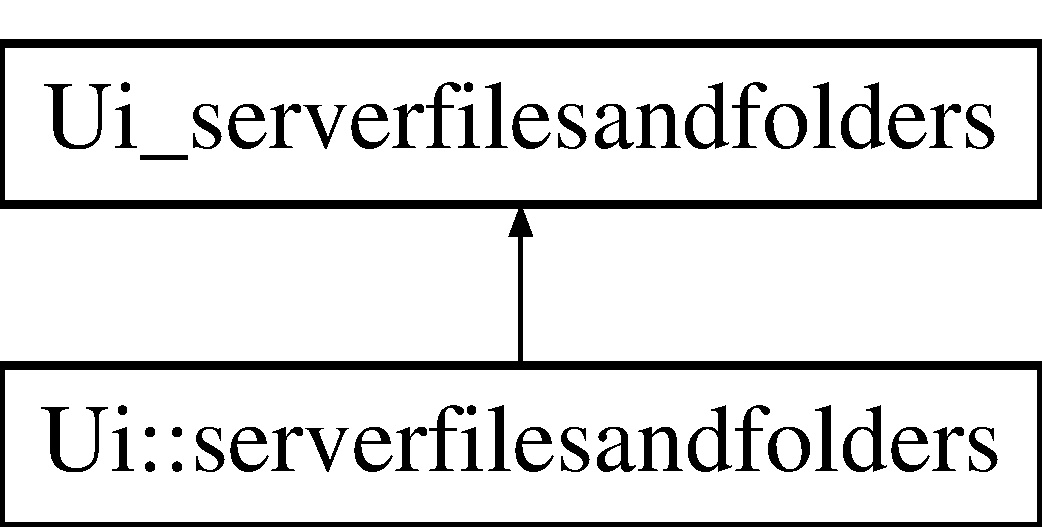
\includegraphics[height=2.000000cm]{classUi__serverfilesandfolders}
\end{center}
\end{figure}
\subsection*{Public Member Functions}
\begin{DoxyCompactItemize}
\item 
void \hyperlink{classUi__serverfilesandfolders_a76af20f8cb4f7ab2eb3ea3ba7ad2c7a6}{setup\-Ui} (Q\-Dialog $\ast$\hyperlink{classserverfilesandfolders}{serverfilesandfolders})
\item 
void \hyperlink{classUi__serverfilesandfolders_aa69fcaab2df41f505801a902f2f951ee}{retranslate\-Ui} (Q\-Dialog $\ast$\hyperlink{classserverfilesandfolders}{serverfilesandfolders})
\end{DoxyCompactItemize}
\subsection*{Public Attributes}
\begin{DoxyCompactItemize}
\item 
Q\-Widget $\ast$ \hyperlink{classUi__serverfilesandfolders_a47a10c1749cf75c7fb9c3aaeea53494e}{layout\-Widget}
\item 
Q\-V\-Box\-Layout $\ast$ \hyperlink{classUi__serverfilesandfolders_a29cf8c53fe60d27322921fde2a072f65}{vertical\-Layout}
\item 
Q\-Label $\ast$ \hyperlink{classUi__serverfilesandfolders_a9c02cefd8fed0f107977e36eb7511b4c}{label}
\item 
Q\-Tree\-View $\ast$ \hyperlink{classUi__serverfilesandfolders_a5e983a9840e30bc26a8b7f0640833c93}{tree\-View}
\item 
Q\-Push\-Button $\ast$ \hyperlink{classUi__serverfilesandfolders_a942d6d5883f0875665471278d70ffee7}{back}
\end{DoxyCompactItemize}


\subsection{Member Function Documentation}
\hypertarget{classUi__serverfilesandfolders_aa69fcaab2df41f505801a902f2f951ee}{\index{Ui\-\_\-serverfilesandfolders@{Ui\-\_\-serverfilesandfolders}!retranslate\-Ui@{retranslate\-Ui}}
\index{retranslate\-Ui@{retranslate\-Ui}!Ui_serverfilesandfolders@{Ui\-\_\-serverfilesandfolders}}
\subsubsection[{retranslate\-Ui}]{\setlength{\rightskip}{0pt plus 5cm}void Ui\-\_\-serverfilesandfolders\-::retranslate\-Ui (
\begin{DoxyParamCaption}
\item[{Q\-Dialog $\ast$}]{serverfilesandfolders}
\end{DoxyParamCaption}
)\hspace{0.3cm}{\ttfamily [inline]}}}\label{classUi__serverfilesandfolders_aa69fcaab2df41f505801a902f2f951ee}
\hypertarget{classUi__serverfilesandfolders_a76af20f8cb4f7ab2eb3ea3ba7ad2c7a6}{\index{Ui\-\_\-serverfilesandfolders@{Ui\-\_\-serverfilesandfolders}!setup\-Ui@{setup\-Ui}}
\index{setup\-Ui@{setup\-Ui}!Ui_serverfilesandfolders@{Ui\-\_\-serverfilesandfolders}}
\subsubsection[{setup\-Ui}]{\setlength{\rightskip}{0pt plus 5cm}void Ui\-\_\-serverfilesandfolders\-::setup\-Ui (
\begin{DoxyParamCaption}
\item[{Q\-Dialog $\ast$}]{serverfilesandfolders}
\end{DoxyParamCaption}
)\hspace{0.3cm}{\ttfamily [inline]}}}\label{classUi__serverfilesandfolders_a76af20f8cb4f7ab2eb3ea3ba7ad2c7a6}


\subsection{Member Data Documentation}
\hypertarget{classUi__serverfilesandfolders_a942d6d5883f0875665471278d70ffee7}{\index{Ui\-\_\-serverfilesandfolders@{Ui\-\_\-serverfilesandfolders}!back@{back}}
\index{back@{back}!Ui_serverfilesandfolders@{Ui\-\_\-serverfilesandfolders}}
\subsubsection[{back}]{\setlength{\rightskip}{0pt plus 5cm}Q\-Push\-Button$\ast$ Ui\-\_\-serverfilesandfolders\-::back}}\label{classUi__serverfilesandfolders_a942d6d5883f0875665471278d70ffee7}
\hypertarget{classUi__serverfilesandfolders_a9c02cefd8fed0f107977e36eb7511b4c}{\index{Ui\-\_\-serverfilesandfolders@{Ui\-\_\-serverfilesandfolders}!label@{label}}
\index{label@{label}!Ui_serverfilesandfolders@{Ui\-\_\-serverfilesandfolders}}
\subsubsection[{label}]{\setlength{\rightskip}{0pt plus 5cm}Q\-Label$\ast$ Ui\-\_\-serverfilesandfolders\-::label}}\label{classUi__serverfilesandfolders_a9c02cefd8fed0f107977e36eb7511b4c}
\hypertarget{classUi__serverfilesandfolders_a47a10c1749cf75c7fb9c3aaeea53494e}{\index{Ui\-\_\-serverfilesandfolders@{Ui\-\_\-serverfilesandfolders}!layout\-Widget@{layout\-Widget}}
\index{layout\-Widget@{layout\-Widget}!Ui_serverfilesandfolders@{Ui\-\_\-serverfilesandfolders}}
\subsubsection[{layout\-Widget}]{\setlength{\rightskip}{0pt plus 5cm}Q\-Widget$\ast$ Ui\-\_\-serverfilesandfolders\-::layout\-Widget}}\label{classUi__serverfilesandfolders_a47a10c1749cf75c7fb9c3aaeea53494e}
\hypertarget{classUi__serverfilesandfolders_a5e983a9840e30bc26a8b7f0640833c93}{\index{Ui\-\_\-serverfilesandfolders@{Ui\-\_\-serverfilesandfolders}!tree\-View@{tree\-View}}
\index{tree\-View@{tree\-View}!Ui_serverfilesandfolders@{Ui\-\_\-serverfilesandfolders}}
\subsubsection[{tree\-View}]{\setlength{\rightskip}{0pt plus 5cm}Q\-Tree\-View$\ast$ Ui\-\_\-serverfilesandfolders\-::tree\-View}}\label{classUi__serverfilesandfolders_a5e983a9840e30bc26a8b7f0640833c93}
\hypertarget{classUi__serverfilesandfolders_a29cf8c53fe60d27322921fde2a072f65}{\index{Ui\-\_\-serverfilesandfolders@{Ui\-\_\-serverfilesandfolders}!vertical\-Layout@{vertical\-Layout}}
\index{vertical\-Layout@{vertical\-Layout}!Ui_serverfilesandfolders@{Ui\-\_\-serverfilesandfolders}}
\subsubsection[{vertical\-Layout}]{\setlength{\rightskip}{0pt plus 5cm}Q\-V\-Box\-Layout$\ast$ Ui\-\_\-serverfilesandfolders\-::vertical\-Layout}}\label{classUi__serverfilesandfolders_a29cf8c53fe60d27322921fde2a072f65}


The documentation for this class was generated from the following file\-:\begin{DoxyCompactItemize}
\item 
\hyperlink{ui__serverfilesandfolders_8h}{ui\-\_\-serverfilesandfolders.\-h}\end{DoxyCompactItemize}

\hypertarget{classUser}{\section{User Class Reference}
\label{classUser}\index{User@{User}}
}


{\ttfamily \#include $<$User.\-h$>$}

\subsection*{Public Member Functions}
\begin{DoxyCompactItemize}
\item 
\hyperlink{classUser_a4a0137053e591fbb79d9057dd7d2283d}{User} ()
\item 
\hyperlink{classUser_a06d689355eff62c15130ffd2f06fdf28}{User} (std\-::string)
\item 
\hyperlink{classUser_a6c50170566109c0476cdceb4f5302c96}{User} (std\-::string, std\-::string)
\item 
std\-::string \hyperlink{classUser_a1bedb71c31d7af1e5a70819aa83e9de4}{Get\-User\-Name} ()
\item 
std\-::string \hyperlink{classUser_aa3447db463d01490433dba5e0af75b7a}{Get\-Password} ()
\item 
void \hyperlink{classUser_aac0cb11a0777bbc88de628ddb9ef8456}{Set\-User\-Name} (std\-::string)
\item 
void \hyperlink{classUser_a44a865bb873d57aab31c0e82150062e8}{Set\-Password} (std\-::string)
\end{DoxyCompactItemize}
\subsection*{Private Attributes}
\begin{DoxyCompactItemize}
\item 
std\-::string \hyperlink{classUser_a37c0392ff3d39a659a153830c97d9105}{User\-Name}
\item 
std\-::string \hyperlink{classUser_a2a7a82b1a850021c64eca35d33ef333e}{Password}
\end{DoxyCompactItemize}


\subsection{Constructor \& Destructor Documentation}
\hypertarget{classUser_a4a0137053e591fbb79d9057dd7d2283d}{\index{User@{User}!User@{User}}
\index{User@{User}!User@{User}}
\subsubsection[{User}]{\setlength{\rightskip}{0pt plus 5cm}User\-::\-User (
\begin{DoxyParamCaption}
{}
\end{DoxyParamCaption}
)}}\label{classUser_a4a0137053e591fbb79d9057dd7d2283d}
\hypertarget{classUser_a06d689355eff62c15130ffd2f06fdf28}{\index{User@{User}!User@{User}}
\index{User@{User}!User@{User}}
\subsubsection[{User}]{\setlength{\rightskip}{0pt plus 5cm}User\-::\-User (
\begin{DoxyParamCaption}
\item[{std\-::string}]{usname}
\end{DoxyParamCaption}
)}}\label{classUser_a06d689355eff62c15130ffd2f06fdf28}
\hypertarget{classUser_a6c50170566109c0476cdceb4f5302c96}{\index{User@{User}!User@{User}}
\index{User@{User}!User@{User}}
\subsubsection[{User}]{\setlength{\rightskip}{0pt plus 5cm}User\-::\-User (
\begin{DoxyParamCaption}
\item[{std\-::string}]{usname, }
\item[{std\-::string}]{pwd}
\end{DoxyParamCaption}
)}}\label{classUser_a6c50170566109c0476cdceb4f5302c96}


\subsection{Member Function Documentation}
\hypertarget{classUser_aa3447db463d01490433dba5e0af75b7a}{\index{User@{User}!Get\-Password@{Get\-Password}}
\index{Get\-Password@{Get\-Password}!User@{User}}
\subsubsection[{Get\-Password}]{\setlength{\rightskip}{0pt plus 5cm}std\-::string User\-::\-Get\-Password (
\begin{DoxyParamCaption}
{}
\end{DoxyParamCaption}
)}}\label{classUser_aa3447db463d01490433dba5e0af75b7a}
\hypertarget{classUser_a1bedb71c31d7af1e5a70819aa83e9de4}{\index{User@{User}!Get\-User\-Name@{Get\-User\-Name}}
\index{Get\-User\-Name@{Get\-User\-Name}!User@{User}}
\subsubsection[{Get\-User\-Name}]{\setlength{\rightskip}{0pt plus 5cm}std\-::string User\-::\-Get\-User\-Name (
\begin{DoxyParamCaption}
{}
\end{DoxyParamCaption}
)}}\label{classUser_a1bedb71c31d7af1e5a70819aa83e9de4}
\hypertarget{classUser_a44a865bb873d57aab31c0e82150062e8}{\index{User@{User}!Set\-Password@{Set\-Password}}
\index{Set\-Password@{Set\-Password}!User@{User}}
\subsubsection[{Set\-Password}]{\setlength{\rightskip}{0pt plus 5cm}void User\-::\-Set\-Password (
\begin{DoxyParamCaption}
\item[{std\-::string}]{New\-Name}
\end{DoxyParamCaption}
)}}\label{classUser_a44a865bb873d57aab31c0e82150062e8}
\hypertarget{classUser_aac0cb11a0777bbc88de628ddb9ef8456}{\index{User@{User}!Set\-User\-Name@{Set\-User\-Name}}
\index{Set\-User\-Name@{Set\-User\-Name}!User@{User}}
\subsubsection[{Set\-User\-Name}]{\setlength{\rightskip}{0pt plus 5cm}void User\-::\-Set\-User\-Name (
\begin{DoxyParamCaption}
\item[{std\-::string}]{New\-Name}
\end{DoxyParamCaption}
)}}\label{classUser_aac0cb11a0777bbc88de628ddb9ef8456}


\subsection{Member Data Documentation}
\hypertarget{classUser_a2a7a82b1a850021c64eca35d33ef333e}{\index{User@{User}!Password@{Password}}
\index{Password@{Password}!User@{User}}
\subsubsection[{Password}]{\setlength{\rightskip}{0pt plus 5cm}std\-::string User\-::\-Password\hspace{0.3cm}{\ttfamily [private]}}}\label{classUser_a2a7a82b1a850021c64eca35d33ef333e}
\hypertarget{classUser_a37c0392ff3d39a659a153830c97d9105}{\index{User@{User}!User\-Name@{User\-Name}}
\index{User\-Name@{User\-Name}!User@{User}}
\subsubsection[{User\-Name}]{\setlength{\rightskip}{0pt plus 5cm}std\-::string User\-::\-User\-Name\hspace{0.3cm}{\ttfamily [private]}}}\label{classUser_a37c0392ff3d39a659a153830c97d9105}


The documentation for this class was generated from the following files\-:\begin{DoxyCompactItemize}
\item 
\hyperlink{User_8h}{User.\-h}\item 
\hyperlink{User_8cpp}{User.\-cpp}\end{DoxyCompactItemize}

\hypertarget{classUserBase}{\section{User\-Base Class Reference}
\label{classUserBase}\index{User\-Base@{User\-Base}}
}


{\ttfamily \#include $<$User\-Base.\-h$>$}

\subsection*{Public Member Functions}
\begin{DoxyCompactItemize}
\item 
\hyperlink{classUserBase_aef178f4f3fd2a97b6221c0ec92c675ae}{User\-Base} ()
\item 
int \hyperlink{classUserBase_a9515e2d3cf822f06641900bb37d997e3}{Get\-Number\-Of\-Users} ()
\item 
std\-::unordered\-\_\-map\\*
$<$ std\-::string, std\-::string $>$ \hyperlink{classUserBase_adcb3f5b10e4889d27285813f8f38c893}{Get\-Users\-List} ()
\item 
void \hyperlink{classUserBase_ac008fbb031432046c7ca431d934301e7}{Set\-Users\-Lists} (std\-::unordered\-\_\-map$<$ std\-::string, std\-::string $>$)
\item 
bool \hyperlink{classUserBase_acc5731f7347d1844a43e761ebe42006f}{Verify\-User\-Credentials} (\hyperlink{classUser}{User})
\item 
bool \hyperlink{classUserBase_ab8a35f8cadaeb61010db846b4fc042f2}{Check\-User\-Exists} (\hyperlink{classUser}{User})
\item 
void \hyperlink{classUserBase_a20daf1309f8151cec9ac8f7f4203bd40}{Insert\-User} (\hyperlink{classUser}{User})
\item 
bool \hyperlink{classUserBase_a1be56d6f223cd39a6fdaba3d1888f19e}{Change\-Password} (std\-::string, std\-::string, std\-::string)
\item 
void \hyperlink{classUserBase_ac9d7a05e0345ef040df653ee0fed6224}{Store\-To\-File} (std\-::string)
\item 
void \hyperlink{classUserBase_aebca8f40b615194c576ef041668b9726}{Load\-From\-File} (std\-::string)
\end{DoxyCompactItemize}
\subsection*{Private Attributes}
\begin{DoxyCompactItemize}
\item 
std\-::unordered\-\_\-map\\*
$<$ std\-::string, std\-::string $>$ \hyperlink{classUserBase_a6e9f1eff5be41e7a37e50b8281270266}{Users\-List}
\end{DoxyCompactItemize}


\subsection{Constructor \& Destructor Documentation}
\hypertarget{classUserBase_aef178f4f3fd2a97b6221c0ec92c675ae}{\index{User\-Base@{User\-Base}!User\-Base@{User\-Base}}
\index{User\-Base@{User\-Base}!UserBase@{User\-Base}}
\subsubsection[{User\-Base}]{\setlength{\rightskip}{0pt plus 5cm}User\-Base\-::\-User\-Base (
\begin{DoxyParamCaption}
{}
\end{DoxyParamCaption}
)}}\label{classUserBase_aef178f4f3fd2a97b6221c0ec92c675ae}


\subsection{Member Function Documentation}
\hypertarget{classUserBase_a1be56d6f223cd39a6fdaba3d1888f19e}{\index{User\-Base@{User\-Base}!Change\-Password@{Change\-Password}}
\index{Change\-Password@{Change\-Password}!UserBase@{User\-Base}}
\subsubsection[{Change\-Password}]{\setlength{\rightskip}{0pt plus 5cm}bool User\-Base\-::\-Change\-Password (
\begin{DoxyParamCaption}
\item[{std\-::string}]{username, }
\item[{std\-::string}]{old\-\_\-password, }
\item[{std\-::string}]{new\-\_\-password}
\end{DoxyParamCaption}
)}}\label{classUserBase_a1be56d6f223cd39a6fdaba3d1888f19e}
\hypertarget{classUserBase_ab8a35f8cadaeb61010db846b4fc042f2}{\index{User\-Base@{User\-Base}!Check\-User\-Exists@{Check\-User\-Exists}}
\index{Check\-User\-Exists@{Check\-User\-Exists}!UserBase@{User\-Base}}
\subsubsection[{Check\-User\-Exists}]{\setlength{\rightskip}{0pt plus 5cm}bool User\-Base\-::\-Check\-User\-Exists (
\begin{DoxyParamCaption}
\item[{{\bf User}}]{User\-Cons}
\end{DoxyParamCaption}
)}}\label{classUserBase_ab8a35f8cadaeb61010db846b4fc042f2}
\hypertarget{classUserBase_a9515e2d3cf822f06641900bb37d997e3}{\index{User\-Base@{User\-Base}!Get\-Number\-Of\-Users@{Get\-Number\-Of\-Users}}
\index{Get\-Number\-Of\-Users@{Get\-Number\-Of\-Users}!UserBase@{User\-Base}}
\subsubsection[{Get\-Number\-Of\-Users}]{\setlength{\rightskip}{0pt plus 5cm}int User\-Base\-::\-Get\-Number\-Of\-Users (
\begin{DoxyParamCaption}
{}
\end{DoxyParamCaption}
)}}\label{classUserBase_a9515e2d3cf822f06641900bb37d997e3}
\hypertarget{classUserBase_adcb3f5b10e4889d27285813f8f38c893}{\index{User\-Base@{User\-Base}!Get\-Users\-List@{Get\-Users\-List}}
\index{Get\-Users\-List@{Get\-Users\-List}!UserBase@{User\-Base}}
\subsubsection[{Get\-Users\-List}]{\setlength{\rightskip}{0pt plus 5cm}std\-::unordered\-\_\-map$<$ std\-::string, std\-::string $>$ User\-Base\-::\-Get\-Users\-List (
\begin{DoxyParamCaption}
{}
\end{DoxyParamCaption}
)}}\label{classUserBase_adcb3f5b10e4889d27285813f8f38c893}
\hypertarget{classUserBase_a20daf1309f8151cec9ac8f7f4203bd40}{\index{User\-Base@{User\-Base}!Insert\-User@{Insert\-User}}
\index{Insert\-User@{Insert\-User}!UserBase@{User\-Base}}
\subsubsection[{Insert\-User}]{\setlength{\rightskip}{0pt plus 5cm}void User\-Base\-::\-Insert\-User (
\begin{DoxyParamCaption}
\item[{{\bf User}}]{User\-Cons}
\end{DoxyParamCaption}
)}}\label{classUserBase_a20daf1309f8151cec9ac8f7f4203bd40}
\hypertarget{classUserBase_aebca8f40b615194c576ef041668b9726}{\index{User\-Base@{User\-Base}!Load\-From\-File@{Load\-From\-File}}
\index{Load\-From\-File@{Load\-From\-File}!UserBase@{User\-Base}}
\subsubsection[{Load\-From\-File}]{\setlength{\rightskip}{0pt plus 5cm}void User\-Base\-::\-Load\-From\-File (
\begin{DoxyParamCaption}
\item[{std\-::string}]{location}
\end{DoxyParamCaption}
)}}\label{classUserBase_aebca8f40b615194c576ef041668b9726}
\hypertarget{classUserBase_ac008fbb031432046c7ca431d934301e7}{\index{User\-Base@{User\-Base}!Set\-Users\-Lists@{Set\-Users\-Lists}}
\index{Set\-Users\-Lists@{Set\-Users\-Lists}!UserBase@{User\-Base}}
\subsubsection[{Set\-Users\-Lists}]{\setlength{\rightskip}{0pt plus 5cm}void User\-Base\-::\-Set\-Users\-Lists (
\begin{DoxyParamCaption}
\item[{std\-::unordered\-\_\-map$<$ std\-::string, std\-::string $>$}]{New\-List}
\end{DoxyParamCaption}
)}}\label{classUserBase_ac008fbb031432046c7ca431d934301e7}
\hypertarget{classUserBase_ac9d7a05e0345ef040df653ee0fed6224}{\index{User\-Base@{User\-Base}!Store\-To\-File@{Store\-To\-File}}
\index{Store\-To\-File@{Store\-To\-File}!UserBase@{User\-Base}}
\subsubsection[{Store\-To\-File}]{\setlength{\rightskip}{0pt plus 5cm}void User\-Base\-::\-Store\-To\-File (
\begin{DoxyParamCaption}
\item[{std\-::string}]{location}
\end{DoxyParamCaption}
)}}\label{classUserBase_ac9d7a05e0345ef040df653ee0fed6224}
\hypertarget{classUserBase_acc5731f7347d1844a43e761ebe42006f}{\index{User\-Base@{User\-Base}!Verify\-User\-Credentials@{Verify\-User\-Credentials}}
\index{Verify\-User\-Credentials@{Verify\-User\-Credentials}!UserBase@{User\-Base}}
\subsubsection[{Verify\-User\-Credentials}]{\setlength{\rightskip}{0pt plus 5cm}bool User\-Base\-::\-Verify\-User\-Credentials (
\begin{DoxyParamCaption}
\item[{{\bf User}}]{User\-Cons}
\end{DoxyParamCaption}
)}}\label{classUserBase_acc5731f7347d1844a43e761ebe42006f}


\subsection{Member Data Documentation}
\hypertarget{classUserBase_a6e9f1eff5be41e7a37e50b8281270266}{\index{User\-Base@{User\-Base}!Users\-List@{Users\-List}}
\index{Users\-List@{Users\-List}!UserBase@{User\-Base}}
\subsubsection[{Users\-List}]{\setlength{\rightskip}{0pt plus 5cm}std\-::unordered\-\_\-map$<$std\-::string, std\-::string$>$ User\-Base\-::\-Users\-List\hspace{0.3cm}{\ttfamily [private]}}}\label{classUserBase_a6e9f1eff5be41e7a37e50b8281270266}


The documentation for this class was generated from the following files\-:\begin{DoxyCompactItemize}
\item 
\hyperlink{UserBase_8h}{User\-Base.\-h}\item 
\hyperlink{UserBase_8cpp}{User\-Base.\-cpp}\end{DoxyCompactItemize}

\chapter{File Documentation}
\hypertarget{allusers_8cpp}{\section{allusers.\-cpp File Reference}
\label{allusers_8cpp}\index{allusers.\-cpp@{allusers.\-cpp}}
}
{\ttfamily \#include \char`\"{}allusers.\-h\char`\"{}}\\*
{\ttfamily \#include \char`\"{}ui\-\_\-allusers.\-h\char`\"{}}\\*
{\ttfamily \#include $<$string$>$}\\*
{\ttfamily \#include $<$iostream$>$}\\*
{\ttfamily \#include $<$vector$>$}\\*
{\ttfamily \#include \char`\"{}User\-Base.\-h\char`\"{}}\\*
\subsection*{Variables}
\begin{DoxyCompactItemize}
\item 
std\-::vector$<$ std\-::string $>$ \hyperlink{allusers_8cpp_abfad81c134d0066d5dd89e1d137d47b3}{listofitems}
\end{DoxyCompactItemize}


\subsection{Variable Documentation}
\hypertarget{allusers_8cpp_abfad81c134d0066d5dd89e1d137d47b3}{\index{allusers.\-cpp@{allusers.\-cpp}!listofitems@{listofitems}}
\index{listofitems@{listofitems}!allusers.cpp@{allusers.\-cpp}}
\subsubsection[{listofitems}]{\setlength{\rightskip}{0pt plus 5cm}std\-::vector$<$std\-::string$>$ listofitems}}\label{allusers_8cpp_abfad81c134d0066d5dd89e1d137d47b3}

\hypertarget{allusers_8h}{\section{allusers.\-h File Reference}
\label{allusers_8h}\index{allusers.\-h@{allusers.\-h}}
}
{\ttfamily \#include $<$Q\-Dialog$>$}\\*
\subsection*{Classes}
\begin{DoxyCompactItemize}
\item 
class \hyperlink{classallusers}{allusers}
\end{DoxyCompactItemize}
\subsection*{Namespaces}
\begin{DoxyCompactItemize}
\item 
\hyperlink{namespaceUi}{Ui}
\end{DoxyCompactItemize}

\hypertarget{FileCompTest_8cpp}{\section{File\-Comp\-Test.\-cpp File Reference}
\label{FileCompTest_8cpp}\index{File\-Comp\-Test.\-cpp@{File\-Comp\-Test.\-cpp}}
}
{\ttfamily \#include $<$fstream$>$}\\*
{\ttfamily \#include $<$vector$>$}\\*
{\ttfamily \#include $<$algorithm$>$}\\*
{\ttfamily \#include $<$iostream$>$}\\*
\subsection*{Macros}
\begin{DoxyCompactItemize}
\item 
\#define \hyperlink{FileCompTest_8cpp_a70ed59adcb4159ac551058053e649640}{S\-I\-Z\-E}~100000
\end{DoxyCompactItemize}
\subsection*{Functions}
\begin{DoxyCompactItemize}
\item 
bool \hyperlink{FileCompTest_8cpp_a6d6dfe1c2fe9455a03a2ba9f7a68bee4}{Equal\-Vector} (std\-::vector$<$ char $>$ file1, std\-::vector$<$ char $>$ file2)
\item 
int \hyperlink{FileCompTest_8cpp_a3c04138a5bfe5d72780bb7e82a18e627}{main} (int argc, char $\ast$$\ast$argv)
\end{DoxyCompactItemize}


\subsection{Macro Definition Documentation}
\hypertarget{FileCompTest_8cpp_a70ed59adcb4159ac551058053e649640}{\index{File\-Comp\-Test.\-cpp@{File\-Comp\-Test.\-cpp}!S\-I\-Z\-E@{S\-I\-Z\-E}}
\index{S\-I\-Z\-E@{S\-I\-Z\-E}!FileCompTest.cpp@{File\-Comp\-Test.\-cpp}}
\subsubsection[{S\-I\-Z\-E}]{\setlength{\rightskip}{0pt plus 5cm}\#define S\-I\-Z\-E~100000}}\label{FileCompTest_8cpp_a70ed59adcb4159ac551058053e649640}


\subsection{Function Documentation}
\hypertarget{FileCompTest_8cpp_a6d6dfe1c2fe9455a03a2ba9f7a68bee4}{\index{File\-Comp\-Test.\-cpp@{File\-Comp\-Test.\-cpp}!Equal\-Vector@{Equal\-Vector}}
\index{Equal\-Vector@{Equal\-Vector}!FileCompTest.cpp@{File\-Comp\-Test.\-cpp}}
\subsubsection[{Equal\-Vector}]{\setlength{\rightskip}{0pt plus 5cm}bool Equal\-Vector (
\begin{DoxyParamCaption}
\item[{std\-::vector$<$ char $>$}]{file1, }
\item[{std\-::vector$<$ char $>$}]{file2}
\end{DoxyParamCaption}
)}}\label{FileCompTest_8cpp_a6d6dfe1c2fe9455a03a2ba9f7a68bee4}
\hypertarget{FileCompTest_8cpp_a3c04138a5bfe5d72780bb7e82a18e627}{\index{File\-Comp\-Test.\-cpp@{File\-Comp\-Test.\-cpp}!main@{main}}
\index{main@{main}!FileCompTest.cpp@{File\-Comp\-Test.\-cpp}}
\subsubsection[{main}]{\setlength{\rightskip}{0pt plus 5cm}int main (
\begin{DoxyParamCaption}
\item[{int}]{argc, }
\item[{char $\ast$$\ast$}]{argv}
\end{DoxyParamCaption}
)}}\label{FileCompTest_8cpp_a3c04138a5bfe5d72780bb7e82a18e627}

\hypertarget{FileHistory_8cpp}{\section{File\-History.\-cpp File Reference}
\label{FileHistory_8cpp}\index{File\-History.\-cpp@{File\-History.\-cpp}}
}
{\ttfamily \#include \char`\"{}File\-History.\-h\char`\"{}}\\*
\subsection*{Functions}
\begin{DoxyCompactItemize}
\item 
std\-::vector$<$ std\-::pair\\*
$<$ std\-::string, int $>$ $>$ \hyperlink{FileHistory_8cpp_a1c0eea02ccc9c8eb9702a64a2ce57519}{Get\-Vector\-Files} (std\-::string location)
\item 
\hyperlink{classFileHistory}{File\-History} \hyperlink{FileHistory_8cpp_a4cc2d1acc9bd32f612f02db360bc0a1b}{Get\-Files\-On\-Disc} (std\-::string location)
\end{DoxyCompactItemize}


\subsection{Function Documentation}
\hypertarget{FileHistory_8cpp_a4cc2d1acc9bd32f612f02db360bc0a1b}{\index{File\-History.\-cpp@{File\-History.\-cpp}!Get\-Files\-On\-Disc@{Get\-Files\-On\-Disc}}
\index{Get\-Files\-On\-Disc@{Get\-Files\-On\-Disc}!FileHistory.cpp@{File\-History.\-cpp}}
\subsubsection[{Get\-Files\-On\-Disc}]{\setlength{\rightskip}{0pt plus 5cm}{\bf File\-History} Get\-Files\-On\-Disc (
\begin{DoxyParamCaption}
\item[{std\-::string}]{location}
\end{DoxyParamCaption}
)}}\label{FileHistory_8cpp_a4cc2d1acc9bd32f612f02db360bc0a1b}
\hypertarget{FileHistory_8cpp_a1c0eea02ccc9c8eb9702a64a2ce57519}{\index{File\-History.\-cpp@{File\-History.\-cpp}!Get\-Vector\-Files@{Get\-Vector\-Files}}
\index{Get\-Vector\-Files@{Get\-Vector\-Files}!FileHistory.cpp@{File\-History.\-cpp}}
\subsubsection[{Get\-Vector\-Files}]{\setlength{\rightskip}{0pt plus 5cm}std\-::vector$<$ std\-::pair$<$std\-::string, int$>$ $>$ Get\-Vector\-Files (
\begin{DoxyParamCaption}
\item[{std\-::string}]{location}
\end{DoxyParamCaption}
)}}\label{FileHistory_8cpp_a1c0eea02ccc9c8eb9702a64a2ce57519}

\hypertarget{FileHistory_8h}{\section{File\-History.\-h File Reference}
\label{FileHistory_8h}\index{File\-History.\-h@{File\-History.\-h}}
}
{\ttfamily \#include $<$boost/filesystem/operations.\-hpp$>$}\\*
{\ttfamily \#include $<$boost/filesystem.\-hpp$>$}\\*
{\ttfamily \#include $<$vector$>$}\\*
{\ttfamily \#include $<$utility$>$}\\*
{\ttfamily \#include $<$string$>$}\\*
{\ttfamily \#include $<$ctime$>$}\\*
{\ttfamily \#include $<$fstream$>$}\\*
\subsection*{Classes}
\begin{DoxyCompactItemize}
\item 
class \hyperlink{classFileHistory}{File\-History}
\end{DoxyCompactItemize}
\subsection*{Functions}
\begin{DoxyCompactItemize}
\item 
std\-::vector$<$ std\-::pair\\*
$<$ std\-::string, int $>$ $>$ \hyperlink{FileHistory_8h_a7462e160c0cfed33f8c874aebd7d8275}{Get\-Vector\-Files} (std\-::string)
\item 
\hyperlink{classFileHistory}{File\-History} \hyperlink{FileHistory_8h_aa94d7e821e3811f1b79ae9587b5b2b51}{Get\-Files\-On\-Disc} (std\-::string)
\end{DoxyCompactItemize}


\subsection{Function Documentation}
\hypertarget{FileHistory_8h_aa94d7e821e3811f1b79ae9587b5b2b51}{\index{File\-History.\-h@{File\-History.\-h}!Get\-Files\-On\-Disc@{Get\-Files\-On\-Disc}}
\index{Get\-Files\-On\-Disc@{Get\-Files\-On\-Disc}!FileHistory.h@{File\-History.\-h}}
\subsubsection[{Get\-Files\-On\-Disc}]{\setlength{\rightskip}{0pt plus 5cm}{\bf File\-History} Get\-Files\-On\-Disc (
\begin{DoxyParamCaption}
\item[{std\-::string}]{}
\end{DoxyParamCaption}
)}}\label{FileHistory_8h_aa94d7e821e3811f1b79ae9587b5b2b51}
\hypertarget{FileHistory_8h_a7462e160c0cfed33f8c874aebd7d8275}{\index{File\-History.\-h@{File\-History.\-h}!Get\-Vector\-Files@{Get\-Vector\-Files}}
\index{Get\-Vector\-Files@{Get\-Vector\-Files}!FileHistory.h@{File\-History.\-h}}
\subsubsection[{Get\-Vector\-Files}]{\setlength{\rightskip}{0pt plus 5cm}std\-::vector$<$ std\-::pair$<$std\-::string, int$>$ $>$ Get\-Vector\-Files (
\begin{DoxyParamCaption}
\item[{std\-::string}]{}
\end{DoxyParamCaption}
)}}\label{FileHistory_8h_a7462e160c0cfed33f8c874aebd7d8275}

\hypertarget{main_8cpp}{\section{main.\-cpp File Reference}
\label{main_8cpp}\index{main.\-cpp@{main.\-cpp}}
}
{\ttfamily \#include \char`\"{}login.\-h\char`\"{}}\\*
{\ttfamily \#include $<$Q\-Application$>$}\\*
{\ttfamily \#include \char`\"{}filesonserver.\-h\char`\"{}}\\*
{\ttfamily \#include \char`\"{}Client\-Combined.\-h\char`\"{}}\\*
\subsection*{Classes}
\begin{DoxyCompactItemize}
\item 
struct \hyperlink{structgraph}{graph}
\end{DoxyCompactItemize}
\subsection*{Functions}
\begin{DoxyCompactItemize}
\item 
void $\ast$ \hyperlink{main_8cpp_a7cabf9ed133276a0c6c754f93b3fcd72}{Start\-Backend} (void $\ast$\hyperlink{newusersignup_8cpp_ad4377e5c259913b2759a7ae9062e630b}{xyz})
\item 
int \hyperlink{main_8cpp_a0ddf1224851353fc92bfbff6f499fa97}{main} (int argc, char $\ast$argv\mbox{[}$\,$\mbox{]})
\end{DoxyCompactItemize}
\subsection*{Variables}
\begin{DoxyCompactItemize}
\item 
bool \hyperlink{main_8cpp_a561b25ad6bd51d83e5a539b862241dbd}{windowshow} = true
\item 
bool \hyperlink{main_8cpp_a27e8a62e7ce6432c2e6cc9ed55b7da40}{Instruction\-Started}
\item 
bool \hyperlink{main_8cpp_a87651879d4fd4c2beb93820231ff862d}{Instruction\-Completed}
\item 
std\-::string \hyperlink{main_8cpp_a9878875765a2eee11b344f7ad57c5c90}{reversedata1}
\item 
std\-::string \hyperlink{main_8cpp_a9292ae8ce70098042c5cf1e510093b66}{reversedata2}
\item 
std\-::string \hyperlink{main_8cpp_a247b1a9d57a29a114c0e2649fc2ae20d}{reversedata3}
\item 
std\-::string \hyperlink{main_8cpp_a0589b412ad453eb8c5dbce0e056c151b}{inst}
\item 
std\-::string \hyperlink{main_8cpp_a838cce38247da46ac6156f1fe05e04e0}{datafield1}
\item 
std\-::string \hyperlink{main_8cpp_aa9d82846c75f7bdf77759c5a08e3bb04}{datafield2}
\item 
std\-::string \hyperlink{main_8cpp_aa9ec05fbafdbff5c987285c2d1e8a405}{datafield3}
\item 
\hyperlink{classSyncManager}{Sync\-Manager} \hyperlink{main_8cpp_a13b2dcfd1eb25bd60ee65d2cab8144ee}{Merged\-Sync\-Manager}
\item 
bool \hyperlink{main_8cpp_a4f5bfd7cc3e09833c6909c379935f84e}{ifconnected}
\item 
std\-::vector$<$ \hyperlink{classData}{Data} $>$ \hyperlink{main_8cpp_a2dd0883ecd227be170d81a3544a1be61}{Reverse\-Data\-Files}
\end{DoxyCompactItemize}


\subsection{Function Documentation}
\hypertarget{main_8cpp_a0ddf1224851353fc92bfbff6f499fa97}{\index{main.\-cpp@{main.\-cpp}!main@{main}}
\index{main@{main}!main.cpp@{main.\-cpp}}
\subsubsection[{main}]{\setlength{\rightskip}{0pt plus 5cm}int main (
\begin{DoxyParamCaption}
\item[{int}]{argc, }
\item[{char $\ast$}]{argv\mbox{[}$\,$\mbox{]}}
\end{DoxyParamCaption}
)}}\label{main_8cpp_a0ddf1224851353fc92bfbff6f499fa97}
\hypertarget{main_8cpp_a7cabf9ed133276a0c6c754f93b3fcd72}{\index{main.\-cpp@{main.\-cpp}!Start\-Backend@{Start\-Backend}}
\index{Start\-Backend@{Start\-Backend}!main.cpp@{main.\-cpp}}
\subsubsection[{Start\-Backend}]{\setlength{\rightskip}{0pt plus 5cm}void$\ast$ Start\-Backend (
\begin{DoxyParamCaption}
\item[{void $\ast$}]{xyz}
\end{DoxyParamCaption}
)}}\label{main_8cpp_a7cabf9ed133276a0c6c754f93b3fcd72}


\subsection{Variable Documentation}
\hypertarget{main_8cpp_a838cce38247da46ac6156f1fe05e04e0}{\index{main.\-cpp@{main.\-cpp}!datafield1@{datafield1}}
\index{datafield1@{datafield1}!main.cpp@{main.\-cpp}}
\subsubsection[{datafield1}]{\setlength{\rightskip}{0pt plus 5cm}std\-::string datafield1}}\label{main_8cpp_a838cce38247da46ac6156f1fe05e04e0}
\hypertarget{main_8cpp_aa9d82846c75f7bdf77759c5a08e3bb04}{\index{main.\-cpp@{main.\-cpp}!datafield2@{datafield2}}
\index{datafield2@{datafield2}!main.cpp@{main.\-cpp}}
\subsubsection[{datafield2}]{\setlength{\rightskip}{0pt plus 5cm}std\-::string datafield2}}\label{main_8cpp_aa9d82846c75f7bdf77759c5a08e3bb04}
\hypertarget{main_8cpp_aa9ec05fbafdbff5c987285c2d1e8a405}{\index{main.\-cpp@{main.\-cpp}!datafield3@{datafield3}}
\index{datafield3@{datafield3}!main.cpp@{main.\-cpp}}
\subsubsection[{datafield3}]{\setlength{\rightskip}{0pt plus 5cm}std\-::string datafield3}}\label{main_8cpp_aa9ec05fbafdbff5c987285c2d1e8a405}
\hypertarget{main_8cpp_a4f5bfd7cc3e09833c6909c379935f84e}{\index{main.\-cpp@{main.\-cpp}!ifconnected@{ifconnected}}
\index{ifconnected@{ifconnected}!main.cpp@{main.\-cpp}}
\subsubsection[{ifconnected}]{\setlength{\rightskip}{0pt plus 5cm}bool ifconnected}}\label{main_8cpp_a4f5bfd7cc3e09833c6909c379935f84e}
\hypertarget{main_8cpp_a0589b412ad453eb8c5dbce0e056c151b}{\index{main.\-cpp@{main.\-cpp}!inst@{inst}}
\index{inst@{inst}!main.cpp@{main.\-cpp}}
\subsubsection[{inst}]{\setlength{\rightskip}{0pt plus 5cm}std\-::string inst}}\label{main_8cpp_a0589b412ad453eb8c5dbce0e056c151b}
\hypertarget{main_8cpp_a87651879d4fd4c2beb93820231ff862d}{\index{main.\-cpp@{main.\-cpp}!Instruction\-Completed@{Instruction\-Completed}}
\index{Instruction\-Completed@{Instruction\-Completed}!main.cpp@{main.\-cpp}}
\subsubsection[{Instruction\-Completed}]{\setlength{\rightskip}{0pt plus 5cm}bool Instruction\-Completed}}\label{main_8cpp_a87651879d4fd4c2beb93820231ff862d}
\hypertarget{main_8cpp_a27e8a62e7ce6432c2e6cc9ed55b7da40}{\index{main.\-cpp@{main.\-cpp}!Instruction\-Started@{Instruction\-Started}}
\index{Instruction\-Started@{Instruction\-Started}!main.cpp@{main.\-cpp}}
\subsubsection[{Instruction\-Started}]{\setlength{\rightskip}{0pt plus 5cm}bool Instruction\-Started}}\label{main_8cpp_a27e8a62e7ce6432c2e6cc9ed55b7da40}
\hypertarget{main_8cpp_a13b2dcfd1eb25bd60ee65d2cab8144ee}{\index{main.\-cpp@{main.\-cpp}!Merged\-Sync\-Manager@{Merged\-Sync\-Manager}}
\index{Merged\-Sync\-Manager@{Merged\-Sync\-Manager}!main.cpp@{main.\-cpp}}
\subsubsection[{Merged\-Sync\-Manager}]{\setlength{\rightskip}{0pt plus 5cm}{\bf Sync\-Manager} Merged\-Sync\-Manager}}\label{main_8cpp_a13b2dcfd1eb25bd60ee65d2cab8144ee}
\hypertarget{main_8cpp_a9878875765a2eee11b344f7ad57c5c90}{\index{main.\-cpp@{main.\-cpp}!reversedata1@{reversedata1}}
\index{reversedata1@{reversedata1}!main.cpp@{main.\-cpp}}
\subsubsection[{reversedata1}]{\setlength{\rightskip}{0pt plus 5cm}std\-::string reversedata1}}\label{main_8cpp_a9878875765a2eee11b344f7ad57c5c90}
\hypertarget{main_8cpp_a9292ae8ce70098042c5cf1e510093b66}{\index{main.\-cpp@{main.\-cpp}!reversedata2@{reversedata2}}
\index{reversedata2@{reversedata2}!main.cpp@{main.\-cpp}}
\subsubsection[{reversedata2}]{\setlength{\rightskip}{0pt plus 5cm}std\-::string reversedata2}}\label{main_8cpp_a9292ae8ce70098042c5cf1e510093b66}
\hypertarget{main_8cpp_a247b1a9d57a29a114c0e2649fc2ae20d}{\index{main.\-cpp@{main.\-cpp}!reversedata3@{reversedata3}}
\index{reversedata3@{reversedata3}!main.cpp@{main.\-cpp}}
\subsubsection[{reversedata3}]{\setlength{\rightskip}{0pt plus 5cm}std\-::string reversedata3}}\label{main_8cpp_a247b1a9d57a29a114c0e2649fc2ae20d}
\hypertarget{main_8cpp_a2dd0883ecd227be170d81a3544a1be61}{\index{main.\-cpp@{main.\-cpp}!Reverse\-Data\-Files@{Reverse\-Data\-Files}}
\index{Reverse\-Data\-Files@{Reverse\-Data\-Files}!main.cpp@{main.\-cpp}}
\subsubsection[{Reverse\-Data\-Files}]{\setlength{\rightskip}{0pt plus 5cm}std\-::vector$<${\bf Data}$>$ Reverse\-Data\-Files}}\label{main_8cpp_a2dd0883ecd227be170d81a3544a1be61}
\hypertarget{main_8cpp_a561b25ad6bd51d83e5a539b862241dbd}{\index{main.\-cpp@{main.\-cpp}!windowshow@{windowshow}}
\index{windowshow@{windowshow}!main.cpp@{main.\-cpp}}
\subsubsection[{windowshow}]{\setlength{\rightskip}{0pt plus 5cm}bool windowshow = true}}\label{main_8cpp_a561b25ad6bd51d83e5a539b862241dbd}

\hypertarget{moc__allusers_8cpp}{\section{moc\-\_\-allusers.\-cpp File Reference}
\label{moc__allusers_8cpp}\index{moc\-\_\-allusers.\-cpp@{moc\-\_\-allusers.\-cpp}}
}
{\ttfamily \#include \char`\"{}allusers.\-h\char`\"{}}\\*
{\ttfamily \#include $<$Qt\-Core/qmetatype.\-h$>$}\\*
\subsection*{Classes}
\begin{DoxyCompactItemize}
\item 
struct \hyperlink{structqt__meta__stringdata__allusers__t}{qt\-\_\-meta\-\_\-stringdata\-\_\-allusers\-\_\-t}
\end{DoxyCompactItemize}
\subsection*{Macros}
\begin{DoxyCompactItemize}
\item 
\#define \hyperlink{moc__allusers_8cpp_a75bb9482d242cde0a06c9dbdc6b83abe}{Q\-T\-\_\-\-M\-O\-C\-\_\-\-L\-I\-T\-E\-R\-A\-L}(idx, ofs, len)
\end{DoxyCompactItemize}


\subsection{Macro Definition Documentation}
\hypertarget{moc__allusers_8cpp_a75bb9482d242cde0a06c9dbdc6b83abe}{\index{moc\-\_\-allusers.\-cpp@{moc\-\_\-allusers.\-cpp}!Q\-T\-\_\-\-M\-O\-C\-\_\-\-L\-I\-T\-E\-R\-A\-L@{Q\-T\-\_\-\-M\-O\-C\-\_\-\-L\-I\-T\-E\-R\-A\-L}}
\index{Q\-T\-\_\-\-M\-O\-C\-\_\-\-L\-I\-T\-E\-R\-A\-L@{Q\-T\-\_\-\-M\-O\-C\-\_\-\-L\-I\-T\-E\-R\-A\-L}!moc_allusers.cpp@{moc\-\_\-allusers.\-cpp}}
\subsubsection[{Q\-T\-\_\-\-M\-O\-C\-\_\-\-L\-I\-T\-E\-R\-A\-L}]{\setlength{\rightskip}{0pt plus 5cm}\#define Q\-T\-\_\-\-M\-O\-C\-\_\-\-L\-I\-T\-E\-R\-A\-L(
\begin{DoxyParamCaption}
\item[{}]{idx, }
\item[{}]{ofs, }
\item[{}]{len}
\end{DoxyParamCaption}
)}}\label{moc__allusers_8cpp_a75bb9482d242cde0a06c9dbdc6b83abe}
{\bfseries Value\-:}
\begin{DoxyCode}
Q\_STATIC\_BYTE\_ARRAY\_DATA\_HEADER\_INITIALIZER\_WITH\_OFFSET(len, \(\backslash\)
    offsetof(\hyperlink{structqt__meta__stringdata__allusers__t}{qt\_meta\_stringdata\_allusers\_t}, stringdata) + ofs \(\backslash\)
        - idx * \textcolor{keyword}{sizeof}(QByteArrayData) \(\backslash\)
    )
\end{DoxyCode}

\hypertarget{moc__onlineusers_8cpp}{\section{moc\-\_\-onlineusers.\-cpp File Reference}
\label{moc__onlineusers_8cpp}\index{moc\-\_\-onlineusers.\-cpp@{moc\-\_\-onlineusers.\-cpp}}
}
{\ttfamily \#include \char`\"{}onlineusers.\-h\char`\"{}}\\*
{\ttfamily \#include $<$Qt\-Core/qbytearray.\-h$>$}\\*
{\ttfamily \#include $<$Qt\-Core/qmetatype.\-h$>$}\\*
\subsection*{Classes}
\begin{DoxyCompactItemize}
\item 
struct \hyperlink{structqt__meta__stringdata__OnlineUsers__t}{qt\-\_\-meta\-\_\-stringdata\-\_\-\-Online\-Users\-\_\-t}
\end{DoxyCompactItemize}
\subsection*{Macros}
\begin{DoxyCompactItemize}
\item 
\#define \hyperlink{moc__onlineusers_8cpp_a75bb9482d242cde0a06c9dbdc6b83abe}{Q\-T\-\_\-\-M\-O\-C\-\_\-\-L\-I\-T\-E\-R\-A\-L}(idx, ofs, len)
\end{DoxyCompactItemize}


\subsection{Macro Definition Documentation}
\hypertarget{moc__onlineusers_8cpp_a75bb9482d242cde0a06c9dbdc6b83abe}{\index{moc\-\_\-onlineusers.\-cpp@{moc\-\_\-onlineusers.\-cpp}!Q\-T\-\_\-\-M\-O\-C\-\_\-\-L\-I\-T\-E\-R\-A\-L@{Q\-T\-\_\-\-M\-O\-C\-\_\-\-L\-I\-T\-E\-R\-A\-L}}
\index{Q\-T\-\_\-\-M\-O\-C\-\_\-\-L\-I\-T\-E\-R\-A\-L@{Q\-T\-\_\-\-M\-O\-C\-\_\-\-L\-I\-T\-E\-R\-A\-L}!moc_onlineusers.cpp@{moc\-\_\-onlineusers.\-cpp}}
\subsubsection[{Q\-T\-\_\-\-M\-O\-C\-\_\-\-L\-I\-T\-E\-R\-A\-L}]{\setlength{\rightskip}{0pt plus 5cm}\#define Q\-T\-\_\-\-M\-O\-C\-\_\-\-L\-I\-T\-E\-R\-A\-L(
\begin{DoxyParamCaption}
\item[{}]{idx, }
\item[{}]{ofs, }
\item[{}]{len}
\end{DoxyParamCaption}
)}}\label{moc__onlineusers_8cpp_a75bb9482d242cde0a06c9dbdc6b83abe}
{\bfseries Value\-:}
\begin{DoxyCode}
Q\_STATIC\_BYTE\_ARRAY\_DATA\_HEADER\_INITIALIZER\_WITH\_OFFSET(len, \(\backslash\)
    offsetof(\hyperlink{structqt__meta__stringdata__OnlineUsers__t}{qt\_meta\_stringdata\_OnlineUsers\_t}, stringdata) + ofs \(\backslash\)
        - idx * \textcolor{keyword}{sizeof}(QByteArrayData) \(\backslash\)
    )
\end{DoxyCode}

\input{moc__server_8cpp}
\hypertarget{moc__serverfilesandfolders_8cpp}{\section{moc\-\_\-serverfilesandfolders.\-cpp File Reference}
\label{moc__serverfilesandfolders_8cpp}\index{moc\-\_\-serverfilesandfolders.\-cpp@{moc\-\_\-serverfilesandfolders.\-cpp}}
}
{\ttfamily \#include \char`\"{}serverfilesandfolders.\-h\char`\"{}}\\*
{\ttfamily \#include $<$Qt\-Core/qbytearray.\-h$>$}\\*
{\ttfamily \#include $<$Qt\-Core/qmetatype.\-h$>$}\\*
\subsection*{Classes}
\begin{DoxyCompactItemize}
\item 
struct \hyperlink{structqt__meta__stringdata__serverfilesandfolders__t}{qt\-\_\-meta\-\_\-stringdata\-\_\-serverfilesandfolders\-\_\-t}
\end{DoxyCompactItemize}
\subsection*{Macros}
\begin{DoxyCompactItemize}
\item 
\#define \hyperlink{moc__serverfilesandfolders_8cpp_a75bb9482d242cde0a06c9dbdc6b83abe}{Q\-T\-\_\-\-M\-O\-C\-\_\-\-L\-I\-T\-E\-R\-A\-L}(idx, ofs, len)
\end{DoxyCompactItemize}


\subsection{Macro Definition Documentation}
\hypertarget{moc__serverfilesandfolders_8cpp_a75bb9482d242cde0a06c9dbdc6b83abe}{\index{moc\-\_\-serverfilesandfolders.\-cpp@{moc\-\_\-serverfilesandfolders.\-cpp}!Q\-T\-\_\-\-M\-O\-C\-\_\-\-L\-I\-T\-E\-R\-A\-L@{Q\-T\-\_\-\-M\-O\-C\-\_\-\-L\-I\-T\-E\-R\-A\-L}}
\index{Q\-T\-\_\-\-M\-O\-C\-\_\-\-L\-I\-T\-E\-R\-A\-L@{Q\-T\-\_\-\-M\-O\-C\-\_\-\-L\-I\-T\-E\-R\-A\-L}!moc_serverfilesandfolders.cpp@{moc\-\_\-serverfilesandfolders.\-cpp}}
\subsubsection[{Q\-T\-\_\-\-M\-O\-C\-\_\-\-L\-I\-T\-E\-R\-A\-L}]{\setlength{\rightskip}{0pt plus 5cm}\#define Q\-T\-\_\-\-M\-O\-C\-\_\-\-L\-I\-T\-E\-R\-A\-L(
\begin{DoxyParamCaption}
\item[{}]{idx, }
\item[{}]{ofs, }
\item[{}]{len}
\end{DoxyParamCaption}
)}}\label{moc__serverfilesandfolders_8cpp_a75bb9482d242cde0a06c9dbdc6b83abe}
{\bfseries Value\-:}
\begin{DoxyCode}
Q\_STATIC\_BYTE\_ARRAY\_DATA\_HEADER\_INITIALIZER\_WITH\_OFFSET(len, \(\backslash\)
    offsetof(\hyperlink{structqt__meta__stringdata__serverfilesandfolders__t}{qt\_meta\_stringdata\_serverfilesandfolders\_t}, 
      stringdata) + ofs \(\backslash\)
        - idx * \textcolor{keyword}{sizeof}(QByteArrayData) \(\backslash\)
    )
\end{DoxyCode}

\hypertarget{onlineusers_8cpp}{\section{onlineusers.\-cpp File Reference}
\label{onlineusers_8cpp}\index{onlineusers.\-cpp@{onlineusers.\-cpp}}
}
{\ttfamily \#include \char`\"{}onlineusers.\-h\char`\"{}}\\*
{\ttfamily \#include \char`\"{}ui\-\_\-onlineusers.\-h\char`\"{}}\\*
\subsection*{Variables}
\begin{DoxyCompactItemize}
\item 
std\-::vector$<$ std\-::string $>$ \hyperlink{onlineusers_8cpp_aea139f16c9d9f61920568a085133dfba}{users\-Log}
\end{DoxyCompactItemize}


\subsection{Variable Documentation}
\hypertarget{onlineusers_8cpp_aea139f16c9d9f61920568a085133dfba}{\index{onlineusers.\-cpp@{onlineusers.\-cpp}!users\-Log@{users\-Log}}
\index{users\-Log@{users\-Log}!onlineusers.cpp@{onlineusers.\-cpp}}
\subsubsection[{users\-Log}]{\setlength{\rightskip}{0pt plus 5cm}std\-::vector$<$std\-::string$>$ users\-Log}}\label{onlineusers_8cpp_aea139f16c9d9f61920568a085133dfba}

\hypertarget{onlineusers_8h}{\section{onlineusers.\-h File Reference}
\label{onlineusers_8h}\index{onlineusers.\-h@{onlineusers.\-h}}
}
{\ttfamily \#include $<$Q\-Dialog$>$}\\*
\subsection*{Classes}
\begin{DoxyCompactItemize}
\item 
class \hyperlink{classOnlineUsers}{Online\-Users}
\end{DoxyCompactItemize}
\subsection*{Namespaces}
\begin{DoxyCompactItemize}
\item 
\hyperlink{namespaceUi}{Ui}
\end{DoxyCompactItemize}

\hypertarget{server_8cpp}{\section{server.\-cpp File Reference}
\label{server_8cpp}\index{server.\-cpp@{server.\-cpp}}
}
{\ttfamily \#include \char`\"{}server.\-h\char`\"{}}\\*
{\ttfamily \#include \char`\"{}allusers.\-h\char`\"{}}\\*
{\ttfamily \#include \char`\"{}ui\-\_\-server.\-h\char`\"{}}\\*
{\ttfamily \#include \char`\"{}onlineusers.\-h\char`\"{}}\\*
{\ttfamily \#include \char`\"{}serverfilesandfolders.\-h\char`\"{}}\\*
{\ttfamily \#include $<$unistd.\-h$>$}\\*
\subsection*{Variables}
\begin{DoxyCompactItemize}
\item 
std\-::string \hyperlink{server_8cpp_a6e4874ccb2e4de9bc5674219c182fa75}{iptodisplay}
\item 
std\-::string \hyperlink{server_8cpp_af9a1bca30ad7f2e84694dad2ba39fed6}{porttodisplay}
\item 
std\-::vector$<$ std\-::string $>$ \hyperlink{server_8cpp_aea139f16c9d9f61920568a085133dfba}{users\-Log}
\item 
char \hyperlink{server_8cpp_a38deedb02dcebac366f97a0879b3be5b}{input}
\end{DoxyCompactItemize}


\subsection{Variable Documentation}
\hypertarget{server_8cpp_a38deedb02dcebac366f97a0879b3be5b}{\index{server.\-cpp@{server.\-cpp}!input@{input}}
\index{input@{input}!server.cpp@{server.\-cpp}}
\subsubsection[{input}]{\setlength{\rightskip}{0pt plus 5cm}char input}}\label{server_8cpp_a38deedb02dcebac366f97a0879b3be5b}
\hypertarget{server_8cpp_a6e4874ccb2e4de9bc5674219c182fa75}{\index{server.\-cpp@{server.\-cpp}!iptodisplay@{iptodisplay}}
\index{iptodisplay@{iptodisplay}!server.cpp@{server.\-cpp}}
\subsubsection[{iptodisplay}]{\setlength{\rightskip}{0pt plus 5cm}std\-::string iptodisplay}}\label{server_8cpp_a6e4874ccb2e4de9bc5674219c182fa75}
\hypertarget{server_8cpp_af9a1bca30ad7f2e84694dad2ba39fed6}{\index{server.\-cpp@{server.\-cpp}!porttodisplay@{porttodisplay}}
\index{porttodisplay@{porttodisplay}!server.cpp@{server.\-cpp}}
\subsubsection[{porttodisplay}]{\setlength{\rightskip}{0pt plus 5cm}std\-::string porttodisplay}}\label{server_8cpp_af9a1bca30ad7f2e84694dad2ba39fed6}
\hypertarget{server_8cpp_aea139f16c9d9f61920568a085133dfba}{\index{server.\-cpp@{server.\-cpp}!users\-Log@{users\-Log}}
\index{users\-Log@{users\-Log}!server.cpp@{server.\-cpp}}
\subsubsection[{users\-Log}]{\setlength{\rightskip}{0pt plus 5cm}std\-::vector$<$std\-::string$>$ users\-Log}}\label{server_8cpp_aea139f16c9d9f61920568a085133dfba}

\hypertarget{server_8h}{\section{server.\-h File Reference}
\label{server_8h}\index{server.\-h@{server.\-h}}
}
{\ttfamily \#include $<$Q\-Main\-Window$>$}\\*
\subsection*{Classes}
\begin{DoxyCompactItemize}
\item 
class \hyperlink{classserver}{server}
\end{DoxyCompactItemize}
\subsection*{Namespaces}
\begin{DoxyCompactItemize}
\item 
\hyperlink{namespaceUi}{Ui}
\end{DoxyCompactItemize}

\hypertarget{Server2_8cpp}{\section{Server2.\-cpp File Reference}
\label{Server2_8cpp}\index{Server2.\-cpp@{Server2.\-cpp}}
}
{\ttfamily \#include $<$iostream$>$}\\*
{\ttfamily \#include $<$cstring$>$}\\*
{\ttfamily \#include $<$sys/socket.\-h$>$}\\*
{\ttfamily \#include $<$netdb.\-h$>$}\\*
{\ttfamily \#include $<$unistd.\-h$>$}\\*
{\ttfamily \#include \char`\"{}User\-Base.\-h\char`\"{}}\\*
{\ttfamily \#include \char`\"{}File\-History.\-h\char`\"{}}\\*
{\ttfamily \#include $<$fstream$>$}\\*
{\ttfamily \#include $<$string$>$}\\*
{\ttfamily \#include $<$vector$>$}\\*
{\ttfamily \#include $<$boost/filesystem/operations.\-hpp$>$}\\*
{\ttfamily \#include $<$boost/filesystem.\-hpp$>$}\\*
{\ttfamily \#include $<$openssl/ssl.\-h$>$}\\*
{\ttfamily \#include $<$openssl/err.\-h$>$}\\*
{\ttfamily \#include $<$pthread.\-h$>$}\\*
\subsection*{Macros}
\begin{DoxyCompactItemize}
\item 
\#define \hyperlink{Server2_8cpp_a70ed59adcb4159ac551058053e649640}{S\-I\-Z\-E}~10000
\item 
\#define \hyperlink{Server2_8cpp_a216b2abde239eb946227cab4973b5bc8}{J\-O\-I\-N}~500
\item 
\#define \hyperlink{Server2_8cpp_a39912bfe2a55f30e269196f9141d845d}{B\-U\-F\-F\-S\-I\-Z\-E}~10000000
\item 
\#define \hyperlink{Server2_8cpp_a2fcfdf60d28725b11b5a3539d3acd0d4}{T\-H\-R\-E\-A\-D\-S}~100
\end{DoxyCompactItemize}
\subsection*{Functions}
\begin{DoxyCompactItemize}
\item 
std\-::vector$<$ std\-::string $>$ \hyperlink{Server2_8cpp_aa973059545666c92f13f87814666696b}{Get\-Files} (std\-::string location)
\item 
bool \hyperlink{Server2_8cpp_a6d6dfe1c2fe9455a03a2ba9f7a68bee4}{Equal\-Vector} (std\-::vector$<$ char $>$ file1, std\-::vector$<$ char $>$ file2)
\item 
int \hyperlink{Server2_8cpp_a8cbe113df3cd3f3debceb281083fb944}{Comp\-Files} (std\-::string file1, std\-::string file2)
\item 
std\-::string \hyperlink{Server2_8cpp_a0cde59c431c055ef0fd880ea2a278498}{To\-Str} (char $\ast$arr)
\item 
std\-::string \hyperlink{Server2_8cpp_aeb012c0f92a559b12246da255db525f9}{File\-Name} (std\-::string filename)
\item 
char $\ast$ \hyperlink{Server2_8cpp_ab07990aa563258ba3ec432e705dff1ee}{To\-Arr} (std\-::string str)
\item 
int \hyperlink{Server2_8cpp_ace691344b7e108cb29f2601ca69f23c1}{is\-Root} ()
\item 
void \hyperlink{Server2_8cpp_a09e2794cde02c0efb1347ea84d047efe}{Load\-Certificates} (S\-S\-L\-\_\-\-C\-T\-X $\ast$\hyperlink{Server2_8cpp_ad5433bcc8a463fb4df3ce5912bb11fe3}{ctx}, char $\ast$Cert\-File, char $\ast$Key\-File)
\item 
void \hyperlink{Server2_8cpp_af195e38cc8e359042b01cd9f3bdc069c}{Show\-Certs} (S\-S\-L $\ast$ssl)
\item 
S\-S\-L\-\_\-\-C\-T\-X $\ast$ \hyperlink{Server2_8cpp_a3c1877898c12a45be136eefa41677825}{Init\-S\-S\-L} ()
\item 
void $\ast$ \hyperlink{Server2_8cpp_aeee490d6285ff72b0b15c76167f66b9f}{Input} (void $\ast$\hyperlink{trying2_8cpp_a589d880006c33afde71782ee91bc502e}{data})
\item 
void $\ast$ \hyperlink{Server2_8cpp_a29f0c634933180f2d2d77e09ac06fd0c}{Client\-Service} (void $\ast$\hyperlink{trying2_8cpp_a589d880006c33afde71782ee91bc502e}{data})
\item 
int \hyperlink{Server2_8cpp_a0ebef4c3fd81802712e3e3c7d1b709cb}{servermain} (int argc, char $\ast$$\ast$argv)
\end{DoxyCompactItemize}
\subsection*{Variables}
\begin{DoxyCompactItemize}
\item 
char \hyperlink{Server2_8cpp_a38deedb02dcebac366f97a0879b3be5b}{input}
\item 
S\-S\-L\-\_\-\-C\-T\-X $\ast$ \hyperlink{Server2_8cpp_ad5433bcc8a463fb4df3ce5912bb11fe3}{ctx}
\item 
bool \hyperlink{Server2_8cpp_ae1f6bf024a2d3cd8afc81295e747ae7f}{close\-Server} =false
\item 
\hyperlink{classUserBase}{User\-Base} \hyperlink{Server2_8cpp_a0ec8c472be2a5fa59d5e333081995ca3}{base} =\hyperlink{classUserBase}{User\-Base}()
\item 
int \hyperlink{Server2_8cpp_ae3ef0df0000dc7d980ef6852a2465ccb}{sock\-I\-D}
\item 
struct addrinfo \hyperlink{Server2_8cpp_a3b26cd515b3c1f3c900281a80c479565}{host\-\_\-info}
\item 
struct addrinfo $\ast$ \hyperlink{Server2_8cpp_af07aa0f353ef6ca5a5fdfa29a226227d}{host\-\_\-info\-\_\-list}
\item 
std\-::vector$<$ std\-::string $>$ \hyperlink{Server2_8cpp_aea139f16c9d9f61920568a085133dfba}{users\-Log}
\item 
std\-::vector$<$ std\-::string $>$ \hyperlink{Server2_8cpp_a3d0740334a4cd6266cc7f11ca2a70998}{all\-Users}
\end{DoxyCompactItemize}


\subsection{Macro Definition Documentation}
\hypertarget{Server2_8cpp_a39912bfe2a55f30e269196f9141d845d}{\index{Server2.\-cpp@{Server2.\-cpp}!B\-U\-F\-F\-S\-I\-Z\-E@{B\-U\-F\-F\-S\-I\-Z\-E}}
\index{B\-U\-F\-F\-S\-I\-Z\-E@{B\-U\-F\-F\-S\-I\-Z\-E}!Server2.cpp@{Server2.\-cpp}}
\subsubsection[{B\-U\-F\-F\-S\-I\-Z\-E}]{\setlength{\rightskip}{0pt plus 5cm}\#define B\-U\-F\-F\-S\-I\-Z\-E~10000000}}\label{Server2_8cpp_a39912bfe2a55f30e269196f9141d845d}
\hypertarget{Server2_8cpp_a216b2abde239eb946227cab4973b5bc8}{\index{Server2.\-cpp@{Server2.\-cpp}!J\-O\-I\-N@{J\-O\-I\-N}}
\index{J\-O\-I\-N@{J\-O\-I\-N}!Server2.cpp@{Server2.\-cpp}}
\subsubsection[{J\-O\-I\-N}]{\setlength{\rightskip}{0pt plus 5cm}\#define J\-O\-I\-N~500}}\label{Server2_8cpp_a216b2abde239eb946227cab4973b5bc8}
\hypertarget{Server2_8cpp_a70ed59adcb4159ac551058053e649640}{\index{Server2.\-cpp@{Server2.\-cpp}!S\-I\-Z\-E@{S\-I\-Z\-E}}
\index{S\-I\-Z\-E@{S\-I\-Z\-E}!Server2.cpp@{Server2.\-cpp}}
\subsubsection[{S\-I\-Z\-E}]{\setlength{\rightskip}{0pt plus 5cm}\#define S\-I\-Z\-E~10000}}\label{Server2_8cpp_a70ed59adcb4159ac551058053e649640}
\hypertarget{Server2_8cpp_a2fcfdf60d28725b11b5a3539d3acd0d4}{\index{Server2.\-cpp@{Server2.\-cpp}!T\-H\-R\-E\-A\-D\-S@{T\-H\-R\-E\-A\-D\-S}}
\index{T\-H\-R\-E\-A\-D\-S@{T\-H\-R\-E\-A\-D\-S}!Server2.cpp@{Server2.\-cpp}}
\subsubsection[{T\-H\-R\-E\-A\-D\-S}]{\setlength{\rightskip}{0pt plus 5cm}\#define T\-H\-R\-E\-A\-D\-S~100}}\label{Server2_8cpp_a2fcfdf60d28725b11b5a3539d3acd0d4}


\subsection{Function Documentation}
\hypertarget{Server2_8cpp_a29f0c634933180f2d2d77e09ac06fd0c}{\index{Server2.\-cpp@{Server2.\-cpp}!Client\-Service@{Client\-Service}}
\index{Client\-Service@{Client\-Service}!Server2.cpp@{Server2.\-cpp}}
\subsubsection[{Client\-Service}]{\setlength{\rightskip}{0pt plus 5cm}void$\ast$ Client\-Service (
\begin{DoxyParamCaption}
\item[{void $\ast$}]{data}
\end{DoxyParamCaption}
)}}\label{Server2_8cpp_a29f0c634933180f2d2d77e09ac06fd0c}
\hypertarget{Server2_8cpp_a8cbe113df3cd3f3debceb281083fb944}{\index{Server2.\-cpp@{Server2.\-cpp}!Comp\-Files@{Comp\-Files}}
\index{Comp\-Files@{Comp\-Files}!Server2.cpp@{Server2.\-cpp}}
\subsubsection[{Comp\-Files}]{\setlength{\rightskip}{0pt plus 5cm}int Comp\-Files (
\begin{DoxyParamCaption}
\item[{std\-::string}]{file1, }
\item[{std\-::string}]{file2}
\end{DoxyParamCaption}
)}}\label{Server2_8cpp_a8cbe113df3cd3f3debceb281083fb944}
\hypertarget{Server2_8cpp_a6d6dfe1c2fe9455a03a2ba9f7a68bee4}{\index{Server2.\-cpp@{Server2.\-cpp}!Equal\-Vector@{Equal\-Vector}}
\index{Equal\-Vector@{Equal\-Vector}!Server2.cpp@{Server2.\-cpp}}
\subsubsection[{Equal\-Vector}]{\setlength{\rightskip}{0pt plus 5cm}bool Equal\-Vector (
\begin{DoxyParamCaption}
\item[{std\-::vector$<$ char $>$}]{file1, }
\item[{std\-::vector$<$ char $>$}]{file2}
\end{DoxyParamCaption}
)}}\label{Server2_8cpp_a6d6dfe1c2fe9455a03a2ba9f7a68bee4}
\hypertarget{Server2_8cpp_aeb012c0f92a559b12246da255db525f9}{\index{Server2.\-cpp@{Server2.\-cpp}!File\-Name@{File\-Name}}
\index{File\-Name@{File\-Name}!Server2.cpp@{Server2.\-cpp}}
\subsubsection[{File\-Name}]{\setlength{\rightskip}{0pt plus 5cm}std\-::string File\-Name (
\begin{DoxyParamCaption}
\item[{std\-::string}]{filename}
\end{DoxyParamCaption}
)}}\label{Server2_8cpp_aeb012c0f92a559b12246da255db525f9}
\hypertarget{Server2_8cpp_aa973059545666c92f13f87814666696b}{\index{Server2.\-cpp@{Server2.\-cpp}!Get\-Files@{Get\-Files}}
\index{Get\-Files@{Get\-Files}!Server2.cpp@{Server2.\-cpp}}
\subsubsection[{Get\-Files}]{\setlength{\rightskip}{0pt plus 5cm}std\-::vector$<$std\-::string$>$ Get\-Files (
\begin{DoxyParamCaption}
\item[{std\-::string}]{location}
\end{DoxyParamCaption}
)}}\label{Server2_8cpp_aa973059545666c92f13f87814666696b}
\hypertarget{Server2_8cpp_a3c1877898c12a45be136eefa41677825}{\index{Server2.\-cpp@{Server2.\-cpp}!Init\-S\-S\-L@{Init\-S\-S\-L}}
\index{Init\-S\-S\-L@{Init\-S\-S\-L}!Server2.cpp@{Server2.\-cpp}}
\subsubsection[{Init\-S\-S\-L}]{\setlength{\rightskip}{0pt plus 5cm}S\-S\-L\-\_\-\-C\-T\-X$\ast$ Init\-S\-S\-L (
\begin{DoxyParamCaption}
{}
\end{DoxyParamCaption}
)}}\label{Server2_8cpp_a3c1877898c12a45be136eefa41677825}
\hypertarget{Server2_8cpp_aeee490d6285ff72b0b15c76167f66b9f}{\index{Server2.\-cpp@{Server2.\-cpp}!Input@{Input}}
\index{Input@{Input}!Server2.cpp@{Server2.\-cpp}}
\subsubsection[{Input}]{\setlength{\rightskip}{0pt plus 5cm}void$\ast$ Input (
\begin{DoxyParamCaption}
\item[{void $\ast$}]{data}
\end{DoxyParamCaption}
)}}\label{Server2_8cpp_aeee490d6285ff72b0b15c76167f66b9f}
\hypertarget{Server2_8cpp_ace691344b7e108cb29f2601ca69f23c1}{\index{Server2.\-cpp@{Server2.\-cpp}!is\-Root@{is\-Root}}
\index{is\-Root@{is\-Root}!Server2.cpp@{Server2.\-cpp}}
\subsubsection[{is\-Root}]{\setlength{\rightskip}{0pt plus 5cm}int is\-Root (
\begin{DoxyParamCaption}
{}
\end{DoxyParamCaption}
)}}\label{Server2_8cpp_ace691344b7e108cb29f2601ca69f23c1}
\hypertarget{Server2_8cpp_a09e2794cde02c0efb1347ea84d047efe}{\index{Server2.\-cpp@{Server2.\-cpp}!Load\-Certificates@{Load\-Certificates}}
\index{Load\-Certificates@{Load\-Certificates}!Server2.cpp@{Server2.\-cpp}}
\subsubsection[{Load\-Certificates}]{\setlength{\rightskip}{0pt plus 5cm}void Load\-Certificates (
\begin{DoxyParamCaption}
\item[{S\-S\-L\-\_\-\-C\-T\-X $\ast$}]{ctx, }
\item[{char $\ast$}]{Cert\-File, }
\item[{char $\ast$}]{Key\-File}
\end{DoxyParamCaption}
)}}\label{Server2_8cpp_a09e2794cde02c0efb1347ea84d047efe}
\hypertarget{Server2_8cpp_a0ebef4c3fd81802712e3e3c7d1b709cb}{\index{Server2.\-cpp@{Server2.\-cpp}!servermain@{servermain}}
\index{servermain@{servermain}!Server2.cpp@{Server2.\-cpp}}
\subsubsection[{servermain}]{\setlength{\rightskip}{0pt plus 5cm}int servermain (
\begin{DoxyParamCaption}
\item[{int}]{argc, }
\item[{char $\ast$$\ast$}]{argv}
\end{DoxyParamCaption}
)}}\label{Server2_8cpp_a0ebef4c3fd81802712e3e3c7d1b709cb}
\hypertarget{Server2_8cpp_af195e38cc8e359042b01cd9f3bdc069c}{\index{Server2.\-cpp@{Server2.\-cpp}!Show\-Certs@{Show\-Certs}}
\index{Show\-Certs@{Show\-Certs}!Server2.cpp@{Server2.\-cpp}}
\subsubsection[{Show\-Certs}]{\setlength{\rightskip}{0pt plus 5cm}void Show\-Certs (
\begin{DoxyParamCaption}
\item[{S\-S\-L $\ast$}]{ssl}
\end{DoxyParamCaption}
)}}\label{Server2_8cpp_af195e38cc8e359042b01cd9f3bdc069c}
\hypertarget{Server2_8cpp_ab07990aa563258ba3ec432e705dff1ee}{\index{Server2.\-cpp@{Server2.\-cpp}!To\-Arr@{To\-Arr}}
\index{To\-Arr@{To\-Arr}!Server2.cpp@{Server2.\-cpp}}
\subsubsection[{To\-Arr}]{\setlength{\rightskip}{0pt plus 5cm}char$\ast$ To\-Arr (
\begin{DoxyParamCaption}
\item[{std\-::string}]{str}
\end{DoxyParamCaption}
)}}\label{Server2_8cpp_ab07990aa563258ba3ec432e705dff1ee}
\hypertarget{Server2_8cpp_a0cde59c431c055ef0fd880ea2a278498}{\index{Server2.\-cpp@{Server2.\-cpp}!To\-Str@{To\-Str}}
\index{To\-Str@{To\-Str}!Server2.cpp@{Server2.\-cpp}}
\subsubsection[{To\-Str}]{\setlength{\rightskip}{0pt plus 5cm}std\-::string To\-Str (
\begin{DoxyParamCaption}
\item[{char $\ast$}]{arr}
\end{DoxyParamCaption}
)}}\label{Server2_8cpp_a0cde59c431c055ef0fd880ea2a278498}


\subsection{Variable Documentation}
\hypertarget{Server2_8cpp_a3d0740334a4cd6266cc7f11ca2a70998}{\index{Server2.\-cpp@{Server2.\-cpp}!all\-Users@{all\-Users}}
\index{all\-Users@{all\-Users}!Server2.cpp@{Server2.\-cpp}}
\subsubsection[{all\-Users}]{\setlength{\rightskip}{0pt plus 5cm}std\-::vector$<$std\-::string$>$ all\-Users}}\label{Server2_8cpp_a3d0740334a4cd6266cc7f11ca2a70998}
\hypertarget{Server2_8cpp_a0ec8c472be2a5fa59d5e333081995ca3}{\index{Server2.\-cpp@{Server2.\-cpp}!base@{base}}
\index{base@{base}!Server2.cpp@{Server2.\-cpp}}
\subsubsection[{base}]{\setlength{\rightskip}{0pt plus 5cm}{\bf User\-Base} base ={\bf User\-Base}()}}\label{Server2_8cpp_a0ec8c472be2a5fa59d5e333081995ca3}
\hypertarget{Server2_8cpp_ae1f6bf024a2d3cd8afc81295e747ae7f}{\index{Server2.\-cpp@{Server2.\-cpp}!close\-Server@{close\-Server}}
\index{close\-Server@{close\-Server}!Server2.cpp@{Server2.\-cpp}}
\subsubsection[{close\-Server}]{\setlength{\rightskip}{0pt plus 5cm}bool close\-Server =false}}\label{Server2_8cpp_ae1f6bf024a2d3cd8afc81295e747ae7f}
\hypertarget{Server2_8cpp_ad5433bcc8a463fb4df3ce5912bb11fe3}{\index{Server2.\-cpp@{Server2.\-cpp}!ctx@{ctx}}
\index{ctx@{ctx}!Server2.cpp@{Server2.\-cpp}}
\subsubsection[{ctx}]{\setlength{\rightskip}{0pt plus 5cm}S\-S\-L\-\_\-\-C\-T\-X$\ast$ ctx}}\label{Server2_8cpp_ad5433bcc8a463fb4df3ce5912bb11fe3}
\hypertarget{Server2_8cpp_a3b26cd515b3c1f3c900281a80c479565}{\index{Server2.\-cpp@{Server2.\-cpp}!host\-\_\-info@{host\-\_\-info}}
\index{host\-\_\-info@{host\-\_\-info}!Server2.cpp@{Server2.\-cpp}}
\subsubsection[{host\-\_\-info}]{\setlength{\rightskip}{0pt plus 5cm}struct addrinfo host\-\_\-info}}\label{Server2_8cpp_a3b26cd515b3c1f3c900281a80c479565}
\hypertarget{Server2_8cpp_af07aa0f353ef6ca5a5fdfa29a226227d}{\index{Server2.\-cpp@{Server2.\-cpp}!host\-\_\-info\-\_\-list@{host\-\_\-info\-\_\-list}}
\index{host\-\_\-info\-\_\-list@{host\-\_\-info\-\_\-list}!Server2.cpp@{Server2.\-cpp}}
\subsubsection[{host\-\_\-info\-\_\-list}]{\setlength{\rightskip}{0pt plus 5cm}struct addrinfo$\ast$ host\-\_\-info\-\_\-list}}\label{Server2_8cpp_af07aa0f353ef6ca5a5fdfa29a226227d}
\hypertarget{Server2_8cpp_a38deedb02dcebac366f97a0879b3be5b}{\index{Server2.\-cpp@{Server2.\-cpp}!input@{input}}
\index{input@{input}!Server2.cpp@{Server2.\-cpp}}
\subsubsection[{input}]{\setlength{\rightskip}{0pt plus 5cm}char input}}\label{Server2_8cpp_a38deedb02dcebac366f97a0879b3be5b}
\hypertarget{Server2_8cpp_ae3ef0df0000dc7d980ef6852a2465ccb}{\index{Server2.\-cpp@{Server2.\-cpp}!sock\-I\-D@{sock\-I\-D}}
\index{sock\-I\-D@{sock\-I\-D}!Server2.cpp@{Server2.\-cpp}}
\subsubsection[{sock\-I\-D}]{\setlength{\rightskip}{0pt plus 5cm}int sock\-I\-D}}\label{Server2_8cpp_ae3ef0df0000dc7d980ef6852a2465ccb}
\hypertarget{Server2_8cpp_aea139f16c9d9f61920568a085133dfba}{\index{Server2.\-cpp@{Server2.\-cpp}!users\-Log@{users\-Log}}
\index{users\-Log@{users\-Log}!Server2.cpp@{Server2.\-cpp}}
\subsubsection[{users\-Log}]{\setlength{\rightskip}{0pt plus 5cm}std\-::vector$<$std\-::string$>$ users\-Log}}\label{Server2_8cpp_aea139f16c9d9f61920568a085133dfba}

\hypertarget{Server2_8h}{\section{Server2.\-h File Reference}
\label{Server2_8h}\index{Server2.\-h@{Server2.\-h}}
}
\subsection*{Functions}
\begin{DoxyCompactItemize}
\item 
int \hyperlink{Server2_8h_af97eb984144fec9a53695381e73e0a2c}{servermain} (int, char $\ast$$\ast$)
\end{DoxyCompactItemize}


\subsection{Function Documentation}
\hypertarget{Server2_8h_af97eb984144fec9a53695381e73e0a2c}{\index{Server2.\-h@{Server2.\-h}!servermain@{servermain}}
\index{servermain@{servermain}!Server2.h@{Server2.\-h}}
\subsubsection[{servermain}]{\setlength{\rightskip}{0pt plus 5cm}int servermain (
\begin{DoxyParamCaption}
\item[{int}]{, }
\item[{char $\ast$$\ast$}]{}
\end{DoxyParamCaption}
)}}\label{Server2_8h_af97eb984144fec9a53695381e73e0a2c}

\hypertarget{serverfilesandfolders_8cpp}{\section{serverfilesandfolders.\-cpp File Reference}
\label{serverfilesandfolders_8cpp}\index{serverfilesandfolders.\-cpp@{serverfilesandfolders.\-cpp}}
}
{\ttfamily \#include \char`\"{}serverfilesandfolders.\-h\char`\"{}}\\*
{\ttfamily \#include \char`\"{}ui\-\_\-serverfilesandfolders.\-h\char`\"{}}\\*

\hypertarget{serverfilesandfolders_8h}{\section{serverfilesandfolders.\-h File Reference}
\label{serverfilesandfolders_8h}\index{serverfilesandfolders.\-h@{serverfilesandfolders.\-h}}
}
{\ttfamily \#include $<$Q\-Dialog$>$}\\*
{\ttfamily \#include $<$Q\-File\-System\-Model$>$}\\*
{\ttfamily \#include $<$Qt\-Core$>$}\\*
{\ttfamily \#include $<$Qt\-Gui$>$}\\*
\subsection*{Classes}
\begin{DoxyCompactItemize}
\item 
class \hyperlink{classserverfilesandfolders}{serverfilesandfolders}
\end{DoxyCompactItemize}
\subsection*{Namespaces}
\begin{DoxyCompactItemize}
\item 
\hyperlink{namespaceUi}{Ui}
\end{DoxyCompactItemize}

\hypertarget{trying2_8cpp}{\section{trying2.\-cpp File Reference}
\label{trying2_8cpp}\index{trying2.\-cpp@{trying2.\-cpp}}
}
{\ttfamily \#include $<$boost/filesystem.\-hpp$>$}\\*
{\ttfamily \#include $<$string$>$}\\*
{\ttfamily \#include $<$iostream$>$}\\*
{\ttfamily \#include $<$vector$>$}\\*
{\ttfamily \#include $<$fstream$>$}\\*
{\ttfamily \#include $<$filesonserver.\-h$>$}\\*
\subsection*{Functions}
\begin{DoxyCompactItemize}
\item 
std\-::vector$<$ Data $>$ int \hyperlink{trying2_8cpp_adeb73fd6e045586978739ab4f5b19497}{main} ()
\end{DoxyCompactItemize}
\subsection*{Variables}
\begin{DoxyCompactItemize}
\item 
std\-::vector$<$ string $>$ \hyperlink{trying2_8cpp_a589d880006c33afde71782ee91bc502e}{data}
\end{DoxyCompactItemize}


\subsection{Function Documentation}
\hypertarget{trying2_8cpp_adeb73fd6e045586978739ab4f5b19497}{\index{trying2.\-cpp@{trying2.\-cpp}!main@{main}}
\index{main@{main}!trying2.cpp@{trying2.\-cpp}}
\subsubsection[{main}]{\setlength{\rightskip}{0pt plus 5cm}std\-::vector$<$Data$>$ int main (
\begin{DoxyParamCaption}
{}
\end{DoxyParamCaption}
)}}\label{trying2_8cpp_adeb73fd6e045586978739ab4f5b19497}


\subsection{Variable Documentation}
\hypertarget{trying2_8cpp_a589d880006c33afde71782ee91bc502e}{\index{trying2.\-cpp@{trying2.\-cpp}!data@{data}}
\index{data@{data}!trying2.cpp@{trying2.\-cpp}}
\subsubsection[{data}]{\setlength{\rightskip}{0pt plus 5cm}std\-::vector$<$string$>$ data}}\label{trying2_8cpp_a589d880006c33afde71782ee91bc502e}

\hypertarget{ui__allusers_8h}{\section{ui\-\_\-allusers.\-h File Reference}
\label{ui__allusers_8h}\index{ui\-\_\-allusers.\-h@{ui\-\_\-allusers.\-h}}
}
{\ttfamily \#include $<$Qt\-Core/\-Q\-Variant$>$}\\*
{\ttfamily \#include $<$Qt\-Widgets/\-Q\-Action$>$}\\*
{\ttfamily \#include $<$Qt\-Widgets/\-Q\-Application$>$}\\*
{\ttfamily \#include $<$Qt\-Widgets/\-Q\-Button\-Group$>$}\\*
{\ttfamily \#include $<$Qt\-Widgets/\-Q\-Dialog$>$}\\*
{\ttfamily \#include $<$Qt\-Widgets/\-Q\-Header\-View$>$}\\*
{\ttfamily \#include $<$Qt\-Widgets/\-Q\-Label$>$}\\*
{\ttfamily \#include $<$Qt\-Widgets/\-Q\-List\-Widget$>$}\\*
{\ttfamily \#include $<$Qt\-Widgets/\-Q\-Push\-Button$>$}\\*
{\ttfamily \#include $<$Qt\-Widgets/\-Q\-V\-Box\-Layout$>$}\\*
{\ttfamily \#include $<$Qt\-Widgets/\-Q\-Widget$>$}\\*
\subsection*{Classes}
\begin{DoxyCompactItemize}
\item 
class \hyperlink{classUi__allusers}{Ui\-\_\-allusers}
\item 
class \hyperlink{classUi_1_1allusers}{Ui\-::allusers}
\end{DoxyCompactItemize}
\subsection*{Namespaces}
\begin{DoxyCompactItemize}
\item 
\hyperlink{namespaceUi}{Ui}
\end{DoxyCompactItemize}

\hypertarget{ui__onlineusers_8h}{\section{ui\-\_\-onlineusers.\-h File Reference}
\label{ui__onlineusers_8h}\index{ui\-\_\-onlineusers.\-h@{ui\-\_\-onlineusers.\-h}}
}
{\ttfamily \#include $<$Qt\-Core/\-Q\-Variant$>$}\\*
{\ttfamily \#include $<$Qt\-Widgets/\-Q\-Action$>$}\\*
{\ttfamily \#include $<$Qt\-Widgets/\-Q\-Application$>$}\\*
{\ttfamily \#include $<$Qt\-Widgets/\-Q\-Button\-Group$>$}\\*
{\ttfamily \#include $<$Qt\-Widgets/\-Q\-Dialog$>$}\\*
{\ttfamily \#include $<$Qt\-Widgets/\-Q\-Header\-View$>$}\\*
{\ttfamily \#include $<$Qt\-Widgets/\-Q\-Label$>$}\\*
{\ttfamily \#include $<$Qt\-Widgets/\-Q\-List\-Widget$>$}\\*
{\ttfamily \#include $<$Qt\-Widgets/\-Q\-Push\-Button$>$}\\*
{\ttfamily \#include $<$Qt\-Widgets/\-Q\-V\-Box\-Layout$>$}\\*
{\ttfamily \#include $<$Qt\-Widgets/\-Q\-Widget$>$}\\*
\subsection*{Classes}
\begin{DoxyCompactItemize}
\item 
class \hyperlink{classUi__OnlineUsers}{Ui\-\_\-\-Online\-Users}
\item 
class \hyperlink{classUi_1_1OnlineUsers}{Ui\-::\-Online\-Users}
\end{DoxyCompactItemize}
\subsection*{Namespaces}
\begin{DoxyCompactItemize}
\item 
\hyperlink{namespaceUi}{Ui}
\end{DoxyCompactItemize}

\hypertarget{ui__server_8h}{\section{ui\-\_\-server.\-h File Reference}
\label{ui__server_8h}\index{ui\-\_\-server.\-h@{ui\-\_\-server.\-h}}
}
{\ttfamily \#include $<$Qt\-Core/\-Q\-Variant$>$}\\*
{\ttfamily \#include $<$Qt\-Widgets/\-Q\-Action$>$}\\*
{\ttfamily \#include $<$Qt\-Widgets/\-Q\-Application$>$}\\*
{\ttfamily \#include $<$Qt\-Widgets/\-Q\-Button\-Group$>$}\\*
{\ttfamily \#include $<$Qt\-Widgets/\-Q\-H\-Box\-Layout$>$}\\*
{\ttfamily \#include $<$Qt\-Widgets/\-Q\-Header\-View$>$}\\*
{\ttfamily \#include $<$Qt\-Widgets/\-Q\-Label$>$}\\*
{\ttfamily \#include $<$Qt\-Widgets/\-Q\-Main\-Window$>$}\\*
{\ttfamily \#include $<$Qt\-Widgets/\-Q\-Push\-Button$>$}\\*
{\ttfamily \#include $<$Qt\-Widgets/\-Q\-Tool\-Bar$>$}\\*
{\ttfamily \#include $<$Qt\-Widgets/\-Q\-V\-Box\-Layout$>$}\\*
{\ttfamily \#include $<$Qt\-Widgets/\-Q\-Widget$>$}\\*
\subsection*{Classes}
\begin{DoxyCompactItemize}
\item 
class \hyperlink{classUi__server}{Ui\-\_\-server}
\item 
class \hyperlink{classUi_1_1server}{Ui\-::server}
\end{DoxyCompactItemize}
\subsection*{Namespaces}
\begin{DoxyCompactItemize}
\item 
\hyperlink{namespaceUi}{Ui}
\end{DoxyCompactItemize}

\hypertarget{ui__serverfilesandfolders_8h}{\section{ui\-\_\-serverfilesandfolders.\-h File Reference}
\label{ui__serverfilesandfolders_8h}\index{ui\-\_\-serverfilesandfolders.\-h@{ui\-\_\-serverfilesandfolders.\-h}}
}
{\ttfamily \#include $<$Qt\-Core/\-Q\-Variant$>$}\\*
{\ttfamily \#include $<$Qt\-Widgets/\-Q\-Action$>$}\\*
{\ttfamily \#include $<$Qt\-Widgets/\-Q\-Application$>$}\\*
{\ttfamily \#include $<$Qt\-Widgets/\-Q\-Button\-Group$>$}\\*
{\ttfamily \#include $<$Qt\-Widgets/\-Q\-Dialog$>$}\\*
{\ttfamily \#include $<$Qt\-Widgets/\-Q\-Header\-View$>$}\\*
{\ttfamily \#include $<$Qt\-Widgets/\-Q\-Label$>$}\\*
{\ttfamily \#include $<$Qt\-Widgets/\-Q\-Push\-Button$>$}\\*
{\ttfamily \#include $<$Qt\-Widgets/\-Q\-Tree\-View$>$}\\*
{\ttfamily \#include $<$Qt\-Widgets/\-Q\-V\-Box\-Layout$>$}\\*
{\ttfamily \#include $<$Qt\-Widgets/\-Q\-Widget$>$}\\*
\subsection*{Classes}
\begin{DoxyCompactItemize}
\item 
class \hyperlink{classUi__serverfilesandfolders}{Ui\-\_\-serverfilesandfolders}
\item 
class \hyperlink{classUi_1_1serverfilesandfolders}{Ui\-::serverfilesandfolders}
\end{DoxyCompactItemize}
\subsection*{Namespaces}
\begin{DoxyCompactItemize}
\item 
\hyperlink{namespaceUi}{Ui}
\end{DoxyCompactItemize}

\hypertarget{User_8cpp}{\section{User.\-cpp File Reference}
\label{User_8cpp}\index{User.\-cpp@{User.\-cpp}}
}
{\ttfamily \#include \char`\"{}User.\-h\char`\"{}}\\*

\hypertarget{User_8h}{\section{User.\-h File Reference}
\label{User_8h}\index{User.\-h@{User.\-h}}
}
{\ttfamily \#include $<$string$>$}\\*
\subsection*{Classes}
\begin{DoxyCompactItemize}
\item 
class \hyperlink{classUser}{User}
\end{DoxyCompactItemize}

\hypertarget{UserBase_8cpp}{\section{User\-Base.\-cpp File Reference}
\label{UserBase_8cpp}\index{User\-Base.\-cpp@{User\-Base.\-cpp}}
}
{\ttfamily \#include \char`\"{}User\-Base.\-h\char`\"{}}\\*
{\ttfamily \#include $<$fstream$>$}\\*
{\ttfamily \#include $<$iostream$>$}\\*
\subsection*{Functions}
\begin{DoxyCompactItemize}
\item 
std\-::string \hyperlink{UserBase_8cpp_ab38ab876a76ea6c7984472e0e2eeb58b}{Encrypt\-Decrypt} (std\-::string Input\-Text)
\end{DoxyCompactItemize}


\subsection{Function Documentation}
\hypertarget{UserBase_8cpp_ab38ab876a76ea6c7984472e0e2eeb58b}{\index{User\-Base.\-cpp@{User\-Base.\-cpp}!Encrypt\-Decrypt@{Encrypt\-Decrypt}}
\index{Encrypt\-Decrypt@{Encrypt\-Decrypt}!UserBase.cpp@{User\-Base.\-cpp}}
\subsubsection[{Encrypt\-Decrypt}]{\setlength{\rightskip}{0pt plus 5cm}std\-::string Encrypt\-Decrypt (
\begin{DoxyParamCaption}
\item[{std\-::string}]{Input\-Text}
\end{DoxyParamCaption}
)}}\label{UserBase_8cpp_ab38ab876a76ea6c7984472e0e2eeb58b}

\hypertarget{UserBase_8h}{\section{User\-Base.\-h File Reference}
\label{UserBase_8h}\index{User\-Base.\-h@{User\-Base.\-h}}
}
{\ttfamily \#include \char`\"{}User.\-h\char`\"{}}\\*
{\ttfamily \#include $<$unordered\-\_\-map$>$}\\*
\subsection*{Classes}
\begin{DoxyCompactItemize}
\item 
class \hyperlink{classUserBase}{User\-Base}
\end{DoxyCompactItemize}

%--- End generated contents ---

% Index
\newpage
\phantomsection
\addcontentsline{toc}{chapter}{Index}
\printindex

\end{document}
